\documentclass[a4paper]{jreport}
\newcommand{\version}{4.3.3}

\title{{\vspace{2cm}{\Large Version \version} }}
\author{\Large Team SCALE\\ UGC working group}
\date{\today}


\usepackage[dvipdfmx]{graphicx}
\usepackage[dvipdfmx]{hyperref}
\usepackage{amsmath}
\usepackage{ascmac}
\usepackage[round]{natbib}
\usepackage{tabularx}
\usepackage{color}
\usepackage{colortbl}
\usepackage{fancybox}
\usepackage{url}
\usepackage{pxjahyper}
\hypersetup{% options for hyperref
 bookmarksopen=true,
 colorlinks=true,
 linkcolor=red,
 citecolor=cyan,
 urlcolor=cyan,
}
%\setlength{\textwidth}{42zw}
%\setlength{\textheight}{40\baselineskip}
\usepackage[top=30mm,bottom=35mm,left=30mm,right=30mm]{geometry}
\usepackage{wallpaper}
%\renewcommand{\thefootnote}{\fnsymbol{footnote}}
\renewcommand{\thefootnote}{*\arabic{footnote})}

\begin{document}
\CenterWallPaper{1.0}{figure/title_wallpaper.eps}
\maketitle
\ClearWallPaper
\ULCornerWallPaper{.1}{figure/scale_logo_final_ULWB.eps}
\tableofcontents

\chapter{概要}
\label{sec:overview}

%==============================================================%
This user's manual is intended for first-time users
of the regional climate/weather forecasting model \scalerm.
The manual is based on
the meteorology/climate library {\scalelib} version \version.
The current version of \scalelib contains a regional model \scalerm
and a global model \scalegm.
%Only a dynamical core is provided for the latter.
This version of the user's manual explains how to use \scalerm in detail.
A description of \scalegm is planned for the next release.

The structure of this document is as follows:
Part \ref{part:overview} provides an overview of \scalelib,
Part \ref{part:install} describes how to install \scalerm
along with the system requirements. Using simple examples,
Chapters \ref{chap:tutorial_ideal} and \ref{chap:tutorial_real}
explain the basic use of \scalerm
using examples of an ideal experiment and an real atmospheric experiment, respectively.
Since these chapters are constructed as a series of tutorials, it is recommended that beginning users of \scalerm read these chapters meticulously.
Parts \ref{part:basic_usel} and \ref{part:advance_use}
describe how to change the model configuration and explain data format and available functions and tools.
Since each section is closed itself basically, these chapter can be utilized as a dictionary.


If you have any questions or comments, please contact us through the users’ mailing list\\ $\langle \verb|scale-users@ml.riken.jp|\rangle$.


\section{What is \scalelib?} \label{subsec:scale_feature}
%--------------------------------------------------------------%

Scalable Computing for Advanced Library and Environment, called {\scalelib}, is a software library that helps conduct research on climate and weather forecasting on any computer with ease. 
This library covers all processes related to such research: 
pre-processing, simulation, post-processing, and analysis. 
It has the following advantages:
\begin{itemize}
\item 
\scalelib is provided as an open-source software under the `` BSD-2 license''. It is free for use, modification, and redistribution, regardless of whether the user is a business or other enterprise.
\item 
\scalelib contains a regional model called the \scalerm ( SCALE-Regional Model ).
\item 
\scalelib prepares various schemes in a component, as outlined in the next section. They can be appropriately chosen according to the desired experiments of users.
\item 
\scalelib provides a framework for physical processes that can be called not only by \scalerm, but also by other numerical models.
\end{itemize}
For the details of the license, the interested reader can refer to the file \texttt{scale-\version/LICENSE} under the main directory. This explanation of its use is also provided on the SCALE webpage (\scaleweb).

In this section, the concept of \scalelib and its relations to actual models are explained. It can be skipped, as it is not related directly to its practical use.

\clearpage
\Item{Relations between \scalelib library and models}

\begin{figure}[htb]
\begin{center}
  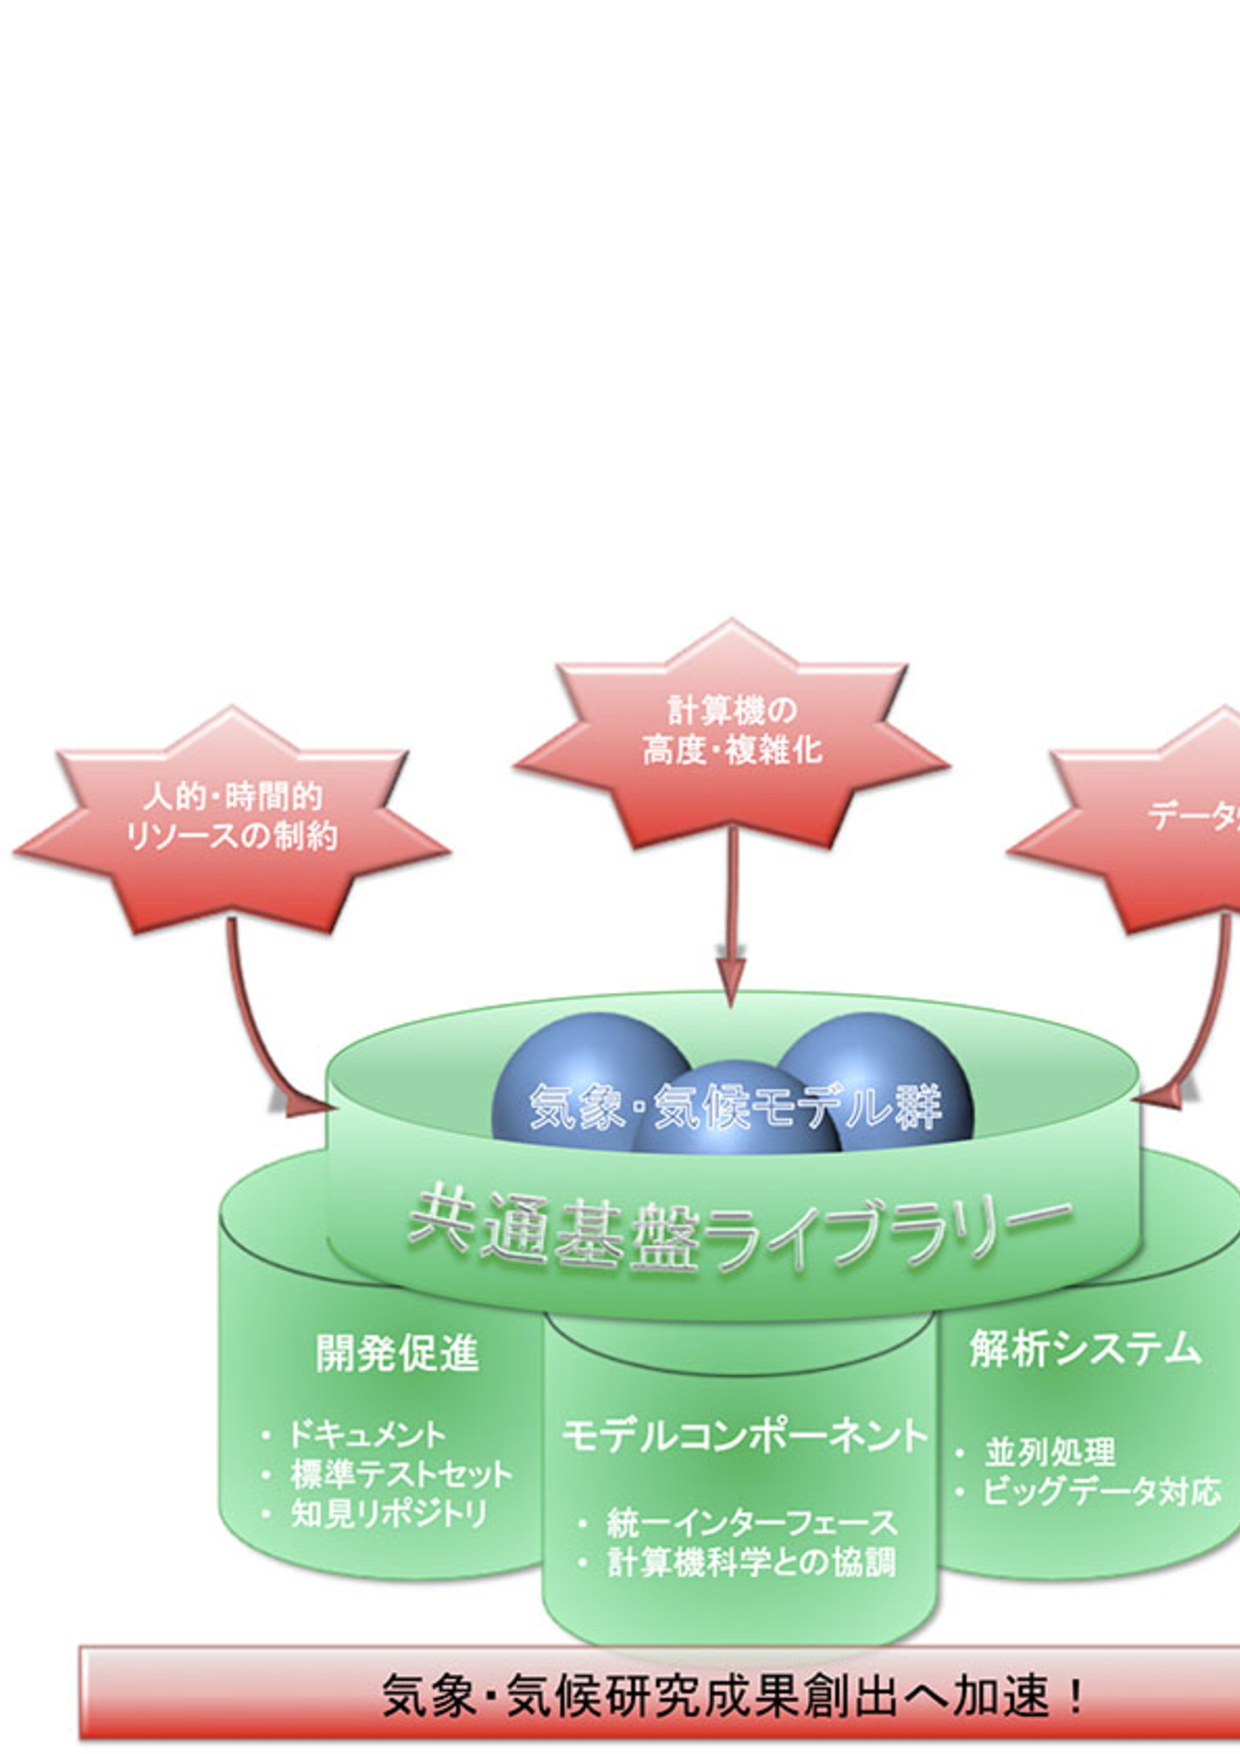
\includegraphics[width=0.9\hsize]{./../../figure/library.pdf}\\
  \caption{Aims of \scalelib}
  \label{fig:scale}
\end{center}
\end{figure}

\scalelib was developed in RIKEN with several outside contributors,
and its improvement and extension continue.
Figure \ref{fig:scale} shows the schematic concept of \scalelib.
As shown in this figure, SCALE aims to resolve various problems.
The development of \scalelib is considered in the context of its wide use
by devices ranging from small PC clusters to next-generation supercomputers.
For this purpose, scientists in meteorology/climate science
and computer science are cooperating.
%This has led to high computational performance of SCALE not only in supercomputers,
%such as the K Computer and the Fujitsu FX10,
%but also for general-purpose commercial computers,
%such as Intel processor-based machines.

\scalerm is a numerical model that fully uses \scalelib.
This model is contained in the \scalelib package,
as shown in Fig. \ref{fig:scale-rm}.
\scalelib manages the parallel processes,
file I/O, and inner-communication.
\scalelib also provides the solver for atmospheric flow ( dynamical core )
and physical processes such as micro-physics and radiation processes.
On the other hand,
\scalerm is constructed by combining functions provided by \scalelib.
\scalerm itself reads the input data of atmospheric status as prognostic variable,
and conducts time-integration.
Users can select a scheme in every component according to simulations they want.

\begin{figure}[hbt]
\begin{center}
  \includegraphics[width=0.9\hsize]{./../../figure/scale.pdf}\\
  \caption{Relationship between the library \scalelib and the model \scalerm}
  \label{fig:scale-rm}
\end{center}
\end{figure}


\section{Structure of \scalerm}  \label{subsec:sturcture_scale_rm}
%--------------------------------------------------------------%
All schemes in all components of \scalelib are available in \scalerm.
The components are categorized into three parts:
framework, dynamical core, and physical processes.
Components with various schemes already implemented
in the current version of \scalerm are listed below\footnote{Refer to \citet{scale_2015},\citet{satoy_2015b}, and \citet{nishizawa_2015} for the details of the model structure and the discretization method.}.

\subsubsection{Framework}
\begin{itemize}
 \item The three-dimensional (3D) Cartesian grid system based on actual distance
 \item 2D domain decomposition by Message Passing Interface (MPI) communication
 \item Several map projections commonly used
 \item Domain nesting system ( one-way, i.e., data transfer from parent domain to child domain. )
   \begin{itemize}
    \item  On-line nesting: concurrent execution of multiple domains).
    \item  Offline nesting: execution of computation in an inner domain after that in an outer domain.
   \end{itemize}
 \item Collective execution system of multiple cases, i.e., bulk job system
 \item \netcdf file I/O based on CF (Climate and Forecast) convention\footnote{\url{http://cfconventions.org/}}
   \begin{itemize}
   \item Selection of {\netcdf}3 and {\netcdf}4 formats
   \end{itemize}
 \item Generation of initial data for an ideal experiment
 \item Generation of topographical and land-use data, converted from external data
 \item Generation of initial and boundary data from external data
   \begin{itemize}
    \item 
      Supporting inputs from the WRF-ARW\footnote{\url{http://www.wrf-model.org/}} and
      \grads \footnote{\url{http://cola.gmu.edu/grads/}} formats.
   \end{itemize}
\end{itemize}

\subsubsection{Dynamical core}
\begin{itemize}
 \item Governing equations: 3D fully compressible non-hydrostatic equations
 \item Spatial discretization: finite volume method
    \begin{itemize}
      \item central advection schemes with 2nd-, 4th-, 6th-order, and 8th-order accuracy
      \item upwind advection schemes with 3rd- , 5th-order, and 7th-order accuracy
    \end{itemize}
 \item Time integration: selection from the ``fully explicit method'' (HEVE)
   or the ``horizontally explicit and vertically implicit methods'' (HEVI)
    \begin{itemize}
      \item \citet{Wicker_2002}'s 3 stage Runge--Kutta scheme with generally 2nd order accuracy
      \item Heun-type 3 stage Runge--Kutta scheme with 3rd order accuracy
      \item 4 stage Runge--Kutta scheme with 4th order accuracy
      \item 7 stage Runge--Kutta scheme with 6th order accuracy (supported only for HEVE)
      \item 11 stage Runge--Kutta scheme with 8th order accuracy (supported only for HEVE)
    \end{itemize}
 \item Guarantee of non-negative value:
    \begin{itemize}
      \item Flux corrected transport method \citep{zalesak_1979}
      \item \citet{Koren_1993}'s filter: available only with the use of the 3rd-order upwind advection scheme
    \end{itemize}
 \item Numerical filter: hyper-viscosity and diffusion with 2nd, 4th, 6th and 8th-order differential operators 
 \item Topography: expressed using terrain-following coordinates
\end{itemize}


\subsubsection{Physical processes}
\begin{itemize}
\item Turbulence process: selectable from among the following
  \begin{itemize}
  \item \citet{smagorinsky_1963} \& \citet{lilly_1962}-type sub-grid scale turbulent model
    with the corrections by \citet{Brown_etal_1994} and \citet{Scotti_1993}
  \item \citet{Deardorff_1980} sub-grid scale turbulent model
  \item MYNN level 2.5 boundary scheme ( \citet{my_1982,nakanishi_2004} )
  \end{itemize}
\item Cloud microphysics: selectable from among the following
  \begin{itemize}
  \item 3-class 1 moment bulk scheme \citep{kessler_1969}
  \item 6-class 1 moment bulk scheme \citep{tomita_2008}
  \item 6-class 2 moment bulk scheme \citep{sn_2014}
  \item spectral bin scheme \citep{suzuki_etal_2010}
  \end{itemize}
\item Radiation process: a k-distribution-based broadband radiation transfer model ( \citet{sekiguchi_2008} )
\item Surface models
  \begin{itemize}
  \item Land model: heat diffusion/bucket model
  \item Ocean model: selectable from among the following
    \begin{itemize}
    \item fixed to initial condition
    \item input from external data
    \item slab model
    \end{itemize}
  \item Urban model: a single-layer canopy model \citep{kusaka_2001}
  \item Heat transfer coefficient at land and in ocean: selectable from among the following
    \begin{itemize}
    \item The bulk method using the universal function \citep{beljaars_1991,wilson_2001}
    \item Louis-type bulk method \citep{uno_1995}
    \end{itemize}
  \end{itemize}
\end{itemize}

\section{Notations used in this document} \label{sec:notation}

This document assumes an execution in the shell ``bash'' on some Unix system.
If your environment is different, replace the commands
by the relevant commands suitable for your environment.
Unless there is a particular remark, this documentation obeys the following notation:

The command-line symbol for execution is expressed by \verb|$| or \verb|#|.
The difference between the two notations is 
in the permission levels of program execution, as shown below:
\begin{verbatim}
 #        <- command by root permission
 $        <- command by user permission
\end{verbatim}

A description enclosed in a rectangle expresses a message generated by the command line, as shown below.
\msgbox{
 -- -- -- -- command-line message\\
 -- -- -- -- -- -- -- -- command-line message\\
 -- -- -- -- -- -- -- -- -- -- -- -- command-line message\\
}

On the other hand, a description enclosed in a polygon with rounded corners means that the description is in an editable file.
\editbox{
 -- -- -- -- description in a file\\
 -- -- -- -- -- -- -- -- description in a file\\
 -- -- -- -- -- -- -- -- -- -- -- -- description in a file\\
}

In this documentation, the FORTRAN namelist and its items are denoted by
\namelist{\it namelist} and \nmitem{\it item_of_namelist}, respectively.



\chapter{インストール}
\label{sec:install}
ここでは,日本域を対象とした実事例実験のチュートリアルを通して,SCALE-LESモデルを実行する一連の作業を説明する.


\section{Installation of SCALE-LES}
%####################################################################################

ここでは,SCALE-LESモデルパッケージを含むSCALEライブラリの
インストール方法を説明する.
SCALEライブラリのインストールに必要となるライブラリ環境のインストール方法については,
必要に応じてAppendix \ref{sec:env_setting}を参照して事前にインストールすること.
以降のチュートリアルでは,Ruby DCL/GPhysに含まれるgpviewがインストールされていると想定して描画の説明を行う.
SCALEのインストールにはコマンドライン端末を使う.コマンドラインのシンボル(\verb|$|)があれば、コマンドの実行を示す.


\subsection{Required Environment}
%====================================================================================

\begin{itemize}
  \item {\bf 計算機環境} : Linux互換OS (Mac OS-Xを含む)が動作する環境.
        マルチコアCPU環境以上を推奨する.
        実験サイズによるが4GB以上のメモリがインストールされているマシン環境が好ましい.
  \item {\bf OS} : Linux OS(Fedora, CentOS, SUSE等),Max OS-X.ここではLinux (CentOS7)を使用して説明する.
  \item {\bf コンパイラ} : Fortran 2003をサポートするC,Fortranコンパイラを必要とする.
        GNU 4.6.x以上,Intel compiler 2012以上を推奨する.ここでは,gcc/gfortranを使用して説明する.
  \item {\bf MPIライブラリ} : MPICH2, OpenMPI, Intel MPI等をサポートする.ここではopenMPIを使用して説明する.
  \item {\bf netcdf3 もしくは HDF5/netcdf4} : gzip, szipをサポートするHDF5,
        およびそのHDF5をサポートするnetcdf4を必要とする.
        ただし,netcdf3の環境下ではscaleライブラリが提供する全ての機能をサポートできない可能性がある.
  \item {\bf 描画環境(非必須)} : Dennou Club提供のRuby DCL/GPhysに含まれるgpview,
        もしくはGrads等の描画環境があると計算結果を簡単にチェックできる.gpviewの使用を推奨する.
  \item SCALEは演算性能評価のためにPAPIライブラリを使用が可能です.
        PAPIライブラリがインストールされている環境下では,
        以下で説明するconfigureファイルの編集によってPAPIを適用することができます.
\end{itemize}



\subsection{Building the source code} \label{sec:source_code}
%====================================================================================

\subsubsection{ソースコードの入手}
%-----------------------------------------------------------------------------------

\url{http://scale.aics.riken.jp/download/scale.tar.gz} の安定版ソースコードのtarballをダウンロードすることができる.
ソースコードのtarballファイルを展開すると\verb|scale/|というディレクトリができる.
以降の説明で\verb|${TOPDIR}|は,scaleディレクトリが存在する絶対PATHを差す.

実事例のシミュレーションを行うには,ソースコードに加えて外部データが必要になる.
このチュートリアル用の気象場のデータ,日本領域の地形・土地利用のデータが収められた
\url{http://scale.aics.riken.jp/download/tutorial_data.tar.gz}も入手し,\verb|${TOPDIR}|の下,
つまりscaleディレクトリと同じ場所に展開しておくこと.\\
\begin{itemize}
 \item \verb|tutorial_data/input_atom| に気象場データ,\\
 \item \verb|tutorial_data/input_topo| に地形データ,\\
 \item \verb|tutorial_data/input_landuse| に土地利用データ\\
\end{itemize}
がそれぞれ格納されている.

\verb|tutorial_data|には,本チュートリアルに必要な最低限のデータのみが納めされているため,
その他の設定で実験を行う場合には別途,気象場,地形,および土地利用データが必要となる.


\subsubsection{configure ファイルと環境変数の設定}
%-----------------------------------------------------------------------------------

\verb|scale/sysdep|内にいくつかのコンフィグファイル(\verb|Makedef.***|)が準備されている.
これらの内から自分の環境にあったものを設定する.
ここでは,OSはLinux,gcc/gfortran コンパイラ,およびopenMPIを使用するため,
\verb|"Makedef.Linux-gnu-ompi"|が設定すべきコンフィグファイルである.
自分の環境に合うものがなければ既存ファイルをベースにして作成する必要がある.
\verb|Makedef.***|の\verb|"***"|の部分を下記のように環境変数として設定する.
\verb|.bashrc|などのファイルに記述しておくと便利である.

また、現実実験のための地形データ、
SCALEをコンパイルするのに必要な外部ライブラリについても下記のようにPATHを設定する.
ここでは,Appendix \ref{sec:env_setting}に従ったとして,
HDF5,netcdf4ともに\verb|/usr|の下にインストールされている場合の例を示す.

\begin{verbatim}
 $ export SCALE_SYS="Linux-gnu-ompi"
 $ export HDF5="/usr"
 $ export NETCDF4="/usr"
\end{verbatim}


\subsubsection{コンパイル}
%-----------------------------------------------------------------------------------

下記のディレクトリに移動して,makeコマンドによってコンパイルを行う.
\begin{verbatim}
 $ cd scale-les/test/tutorial/bin
 $ make -j 4
\end{verbatim}

\verb|make|のあとの \verb|"-j 4"| は,並列コンパイルを指示するオプションで,4並列コンパイルを行うことを指示する.
コンパイルを実行する環境によっては並列数を増やすこともできる.

このmakeによってSCALEライブラリ,およびSCALE-LESモデルのコンパイルが行われ,結果として
\verb|scale-les, scale-les_init, scale-les_pp|の3つの実行ファイルが生成されていればコンパイルは成功である.


{\bf 注意点}
\begin{itemize}
\item SCALEライブラリは,scaleのTOPディレクトリ直下の\verb|scale/scalelib/|というディレクトリ内でコンパイルと
アーカイブが行われ,\verb|"./lib"|という名前の隠しディレクトリとして\verb|bin/|ディレクトリ内へコピーされている.\\
\item Debugモードでコンパイルしたい場合や,コンパイルオプションを変更したい場合は,
      \verb|Makedef.***|のファイルを編集してください.
\item 開発版ソースコードをコンパイルしている場合,一部のコンパイラバージョンにおいて
      コンパイルが正常に終了しないケースがあります.そのような場合はぜひSCALE開発チームまでご報告ください.
\end{itemize}



%####################################################################################



\chapter{チュートリアル: 理想実験}
\label{sec:tuto_ideal}
%%%%%%%%%%%%%%%%%%%%%%%%%%%%%%%%%%%%%%%%%%%%%%%%%%%%%%%%%%%%%%%%%%%%%
%  File 31_ideal_exp.tex
%%%%%%%%%%%%%%%%%%%%%%%%%%%%%%%%%%%%%%%%%%%%%%%%%%%%%%%%%%%%%%%%%%%%%

\section{概要}

本章では、SCALEを使った理想実験の実行方法を説明する。
第\ref{sec:install}章で実行したSCALEのコンパイルが
正常に完了しているかどうかのチェックも含めてぜひ実施してもらいたい。


\subsection{チュートリアル実行のための推奨環境}
\label{sec:assumed_env}

本書のチュートリアルの説明は、下記の環境を前提として記述している。
コンパイラ、ライブラリについては、適宜、使用環境に合わせて読み替えること。

\begin{itemize}
 \item {\bf CPU} : 物理コアが2コア以上 %[Intel Core i5 2410M 2.3GHz 2コア/4スレッド] %、第\ref{sec:tuto_real}章は4コアを搭載
 \item {\bf Memory} : 512MB以上 %[DDR3-1333 4GB]     %、第\ref{sec:tuto_real}章は2GB
 \item {\bf OS} : Linux OS x86-64  %[CentOS 6.6、CentOS 7.1、openSUSE 13.2のいずれか]
 \item {\bf コンパイラ} : GNU コンパイラ(gcc/gfortran)
 \item {\bf MPIライブラリ} : openMPI(リポジトリ経由でのインストール)
\end{itemize}

本章では、SCALEのコンパイルが正常に終了し、
すでに下記のファイルが生成されているものとして説明を行う。
\begin{verbatim} 
  scale/scale-rm/test/tutorial/bin/scale-rm
  scale/scale-rm/test/tutorial/bin/scale-rm_init
  scale/scale-rm/util/netcdf2grads_h/net2g
\end{verbatim}
これらに加えて、本章のチュートリアルでは、
描画ツールとしてgpviewとGrADSを使用する。
gpview(Gphys)とGrADSの詳細やインストール方法については、
付録 \ref{sec:env_vis_tools}節を参照のこと。


\subsection{実験設定}
%====================================================================================

実験設定として、「スコールライン」の理想実験を例にあげる。
この実験では、積乱雲が発生するときの
典型的な大気の鉛直プロファイルと対流圏下層に初期擾乱を与え、
積乱雲が発達する様子を準2次元モデルで実験する内容となっている。
実験設定は表\ref{tab:setting_ideal}に示す通りである。

\begin{table}[htb]
\begin{center}
\caption{チュートリアル理想実験の実験設定}
\begin{tabularx}{150mm}{|l|X|X|} \hline
 \rowcolor[gray]{0.9} 項目 & 設定内容 & 備考 \\ \hline
 水平格子間隔 & 東西:500 m、南北:1000 m & 東西-鉛直の面を切り取った準2次元実験である \\ \hline
 水平格子点数 & 東西:40、南北:2\footnotemark &  \\ \hline
 鉛直層数     & 97層(トップ:20 km)& 下層ほど細かい層間隔をとったストレッチ設定である \\ \hline
 側面境界条件 & 周期境界 & 東西、南北とも \\ \hline
 積分時間間隔 & 5 sec      & 雲微物理スキームは10 sec毎 \\ \hline
 積分期間     & 3,600 sec  & 720 steps \\ \hline
 データ出力間隔 & 300 sec  &  \\ \hline
 物理スキーム & 雲微物理モデルのみ使用 &
 6-class single moment bulk model \citep{tomita_2008} \\ \hline
 初期鉛直プロファイル & GCSS Case1 squall-line \citep{Redelsperger2000}&
 風のプロファイルは、\citet{Ooyama_2001}に基づいた鉛直シアを与える \\ \hline
 初期擾乱 & ウォームバブル & 水平半径4 km、
 鉛直半径3 kmの大きさを持つ最大プラス3Kの強度のウォームバブルを置く\\ \hline
\end{tabularx}
\label{tab:setting_ideal}
\end{center}
\end{table}
\footnotetext{現在は2次元実験を行うための枠組みは用意されていないが、y方向に同じ値をもつ初期値を与える事で2次元実験に相当する実験を行うことが可能である。この場合、ハロの格子数と同じ数の格子数をy方向に設定する必要がある。ハロの必要格子数については\ref{sec:dyn}参照。}



\section{実行方法}
%====================================================================================

実行の流れとしては、前準備、初期値の作成、モデル本体の実行、
後処理、そして描画といった順番で作業を進める。

\subsection{前準備}
%------------------------------------------------------
チュートリアル理想実験は、\verb|scale-rm/test/tutorial/ideal|の
ディレクトリにて実行する。
\begin{verbatim}
  $ cd scale-rm/test/tutorial/ideal
\end{verbatim}
次に、このディレクトリに、
SCALEの実行バイナリの静的リンクを張る。
\begin{verbatim}
  $ ln -s ../bin/scale-rm       ./
  $ ln -s ../bin/scale-rm_init  ./
\end{verbatim}
``\verb|scale-rm|''はモデル本体、
``\verb|scale-rm_init|''は初期値・境界値作成ツールである。
%もし、ここで説明するディレクトリとは異なる場所で実行している場合は、
%リンクを張る時のディレクトリ指定に注意すること。


\subsection{初期値作成}
%------------------------------------------------------
初期値の作成は、``\verb|scale-rm_init|''に
設定ファイル (configファイル)を与えて実行する。
``\verb|init_R20kmDX500m.conf|''には、
表\ref{tab:setting_ideal}に対応した実験設定が書き込まれている。
このconfigファイルを\verb|scale-rm_init|に与えることで、
設定ファイルの指示に従って大気の成層構造を計算し、
初期擾乱が設定される。


SCALEの基本的な実行コマンドは下記のとおりである。
\begin{verbatim}
  $ mpirun  -n  [プロセス数]  [実行バイナリ名]  [configファイル]
\end{verbatim}
[プロセス数]の部分にはMPI並列で使用したいプロセス数を記述する。
[実行バイナリ]には、\verb|scale-rm|や\verb|scale-rm_init|が入る。
そして、実験設定を記述したconfigファイルを
[configファイル]の部分に指定する。
%
例えば、
configファイルに\verb|init_R20kmDX500m.conf|を用いて、
2-MPI並列(2つのMPIプロセス)
で\verb|scale-rm_init|を実行する場合、
コマンドは次のようになる。
\begin{verbatim}
  $ mpirun  -n  2  ./scale-rm_init  init_R20kmDX500m.conf
\end{verbatim}
%
\noindent 実行が成功した場合には、コマンドラインのメッセージは
下記のように表示される。\\

\noindent {\small {\gt
\fbox{
\begin{tabularx}{140mm}{l}
 *** Start Launch System for SCALE-RM\\
 TOTAL BULK JOB NUMBER   =    1\\
 PROCESS NUM of EACH JOB =     2\\
 TOTAL DOMAIN NUMBER     =    1\\
 Flag of ABORT ALL JOBS  =  F\\
 *** a single comunicator\\
 *** a single comunicator\\
\end{tabularx}
}}}\\

\noindent この実行によって、\\
\begin{verbatim}
  init\_LOG.pe000000
  init\_00000000000.000.pe000000.nc
  init\_00000000000.000.pe000001.nc
\end{verbatim}
の3つのファイルが、現在のディレクトリ下に作成される。
``init\_LOG.pe000000''には、
コマンドラインには表示されない詳しい実行ログが記録されている。
実行が正常に終了している場合、このLOGファイルの最後に\\

\noindent {\small {\gt
\ovalbox{
\begin{tabularx}{140mm}{l}
 ++++++ Stop MPI\\
 *** Broadcast STOP signal\\
 *** MPI is peacefully finalized\\
\end{tabularx}
}}}\\

\noindent と記述される。

``init\_00000000000.000.pe000000.nc''と``init\_00000000000.000.pe000001.nc''の
2つのファイルは初期値ファイルである。
計算領域全体を2つのMPIプロセスで分割し担当するため、
2つのファイルが生成される。
もし、4-MPI並列で実行すれば、4つの初期値ファイルが生成される。
これらのファイル名の末尾が``.nc''で終わるファイルは
NetCDF形式のファイルであり、
Gphys/Ruby-DCLやncviewといったツールで直接読むことができる。


\subsection{モデル本体の実行}
%------------------------------------------------------
並列数は、初期値作成のときと同じ数を指定する。
configファイルには``\verb|run_R20kmDX500m.conf|''を指定する。
\begin{verbatim}
  $ mpirun  -n  2  ./scale-rm  run_R20kmDX500m.conf
\end{verbatim}

本書の必要要件にあった計算機であれば、2分程度で計算が終わる。
\noindent この実行によって、\\
\begin{verbatim}
  LOG.pe000000
  history.pe000000.nc
  history.pe000001.nc
  monitor.pe000000
\end{verbatim}
の4つのファイルが、現在のディレクトリ下に作成されているはずである。
``LOG.pe000000''には、
コマンドラインには表示されない詳しい実行ログが記録されている。
実行が正常に終了している場合、このLOGファイルの最後に\\

\noindent {\small {\gt
\ovalbox{
\begin{tabularx}{140mm}{l}
 ++++++ Stop MPI\\
 *** Broadcast STOP signal\\
 *** MPI is peacefully finalized\\
\end{tabularx}
}}}\\

\noindent と記述される。
``history.pe000000.nc''と``history.pe000001.nc''
の2つのファイルが計算結果が記録されたhistoryファイルである。
2-MPI並列で実行したため、2つのファイルが生成されており、
ファイル形式はNetCDFである。
``monitor.pe000000''は、計算中にモニタリングしている
物理変数の時間変化を記録したテキストファイルである。



\subsection{後処理と描画}
%------------------------------------------------------
ここでは、計算結果を描画するための後処理について説明する。本書のチュートリアルでは、
NetCDF形式の分散ファイルを1つのファイルにまとめ、ユーザーが解析しやすいDirect-Accessの
単純バイナリ形式(GrADS形式)に変換する方法を説明する。
%Gphys/Ruby-DCLを使うと
%分割ファイルのまま直接描画することができるが、この方法については\ref{sec:quicklook}節を
%参照してもらいたい。

まず、\ref{sec:source_net2g}節でコンパイルした後処理ツール``net2g''を、
現在のディレクトリへリンクを張る。
\begin{verbatim}
  $ ln -s ../../../util/netcdf2grads_h/net2g  ./
\end{verbatim}
もし、ここで説明するディレクトリとは異なる場所で実行している場合は、
リンクを張る時のディレクトリ指定に注意すること。

net2gも実行方法は基本的にSCALE本体と同じである。
\begin{verbatim}
  $ mpirun  -n  [プロセス数]  ./net2g  [configファイル]
\end{verbatim}
net2g専用の``\verb|net2g.conf|''をconfigファイルとして与えて、
つぎのように実行する。
\begin{verbatim}
  $ mpirun  -n  2  ./net2g  net2g.conf
\end{verbatim}

\noindent net2gの実行にあたっては、SCALE本体の実行時に使用したMPIプロセス数と同じか、
その約数のプロセス数を用いて実行しなければならない。
%HDDの読み書き速度に依存するが、本書の必要要件にあった計算機であれば2分程度で計算が終わる。
この実行によって、書き6つのファイルが、実行ディレクトリ下に作成される。
\begin{verbatim}
  QHYD_d01z-3d.ctl
  QHYD_d01z-3d.grd
  U_d01z-3d.ctl
  U_d01z-3d.grd
  W_d01z-3d.ctl
  W_d01z-3d.grd
\end{verbatim}
これらのファイルはぞれぞれ、
U(水平風東西成分)、W(鉛直風)、QHYD(全凝結物混合比)について、
分割ファイルを1つにまとめ、Direct-Accessの単純バイナリ形式(GrADS形式)に
変換したgrdファイルとGrADSに読み込ませるためのctlファイルである。
従って、このctlファイルをGrADSに読み込ませれば
直ちに計算結果の描画が可能である。
図\ref{fig_ideal}は、積分開始1200秒後における、
U-WとQHYDについての鉛直断面図である。


``\verb|net2g.conf|''の下記の行を編集することによって、
他の変数についても変換が可能である。\\

\noindent {\small {\gt
\ovalbox{
\begin{tabularx}{140mm}{l}
\verb|&VARI|\\
\verb| VNAME       = "U","W","QHYD"|\\
\verb|/|\\
\end{tabularx}
}}}\\

\noindent この``VNAME''の項目を例えば、
\verb|"PT","RH"|と変更して実行すれば温位と相対湿度の変数に
ついて変換する。どの変数が出力されているのかを調べるには、NetCDFのncdumpツールなどを
使えば簡単に調べられる。net2gの詳しい使用方法は、\ref{sec:net2g}を参照してほしい。


\begin{figure}[t]
\begin{center}
  \includegraphics[width=1.0\hsize]{./figure/grads_hist_ideal.eps}\\
  \caption{積分開始後 1200 sec のY=1 kmにおける東西-鉛直断面図;
           (a)のカラーシェードは全凝結物の混合比、
           (b)は鉛直速度をそれぞれ示す。ベクトルは東西-鉛直断面内の風の流れを表す。}
  \label{fig_ideal}
\end{center}
\end{figure}




\subsubsection{この章の最後に}

本章では、スコールラインの理想実験を例に、SCALEの実行方法について説明した。
次ステップとして、
解像度や計算領域、MPIプロセス数の変更
放射過程や乱流過程、雲微物理スキームといった物理過程の変更を
試すことをお勧めする。
これらの変更方法は、第\ref{sec:basic}章に記載されている。

このスコールラインの理想実験については、
同じディレクトリ下の``sample''ディレクトリ内に、
解像度設定、領域設定、使用する物理スキームについて変更を加えたconfigファイルのサンプルが用意されているので、
これらも参考となる。
また、SCALEには各種理想実験セットが``\verb|scale-rm/test/case|''以下に複数用意されている。
ディレクトリ構造がチュートリアルとは
異なる部分もあるが、実行手順は基本的に本章のチュートリアルと同じである。




\chapter{チュートリアル: 現実実験}
\label{sec:tuto_real}

このチュートリアルでは、図 \ref{fig:domain}に示した
領域を対象とした現実大気実験を行う。
現実大気実験用のチュートリアルは
\begin{verbatim}
 scale/scale-les/test/tutorial/real/
\end{verbatim}
の下で行う。
以降の説明で\verb|${Tutrial_DIR}|は、\verb|scale/scale-les/test/tutorial/|を絶対PATHで示すこととする。

SCALE-LESモデルの実行過程は、図 \ref{fig:howto}に示されるように
\begin{enumerate}
\item pp : 地形・海陸分布データの作成
\item init : 初期値・境界値データの作成
\item run : 時間積分を行う(モデル本体の実行)
\end{enumerate}
といった手順で実行する。


\begin{figure}[h]
\begin{center}
  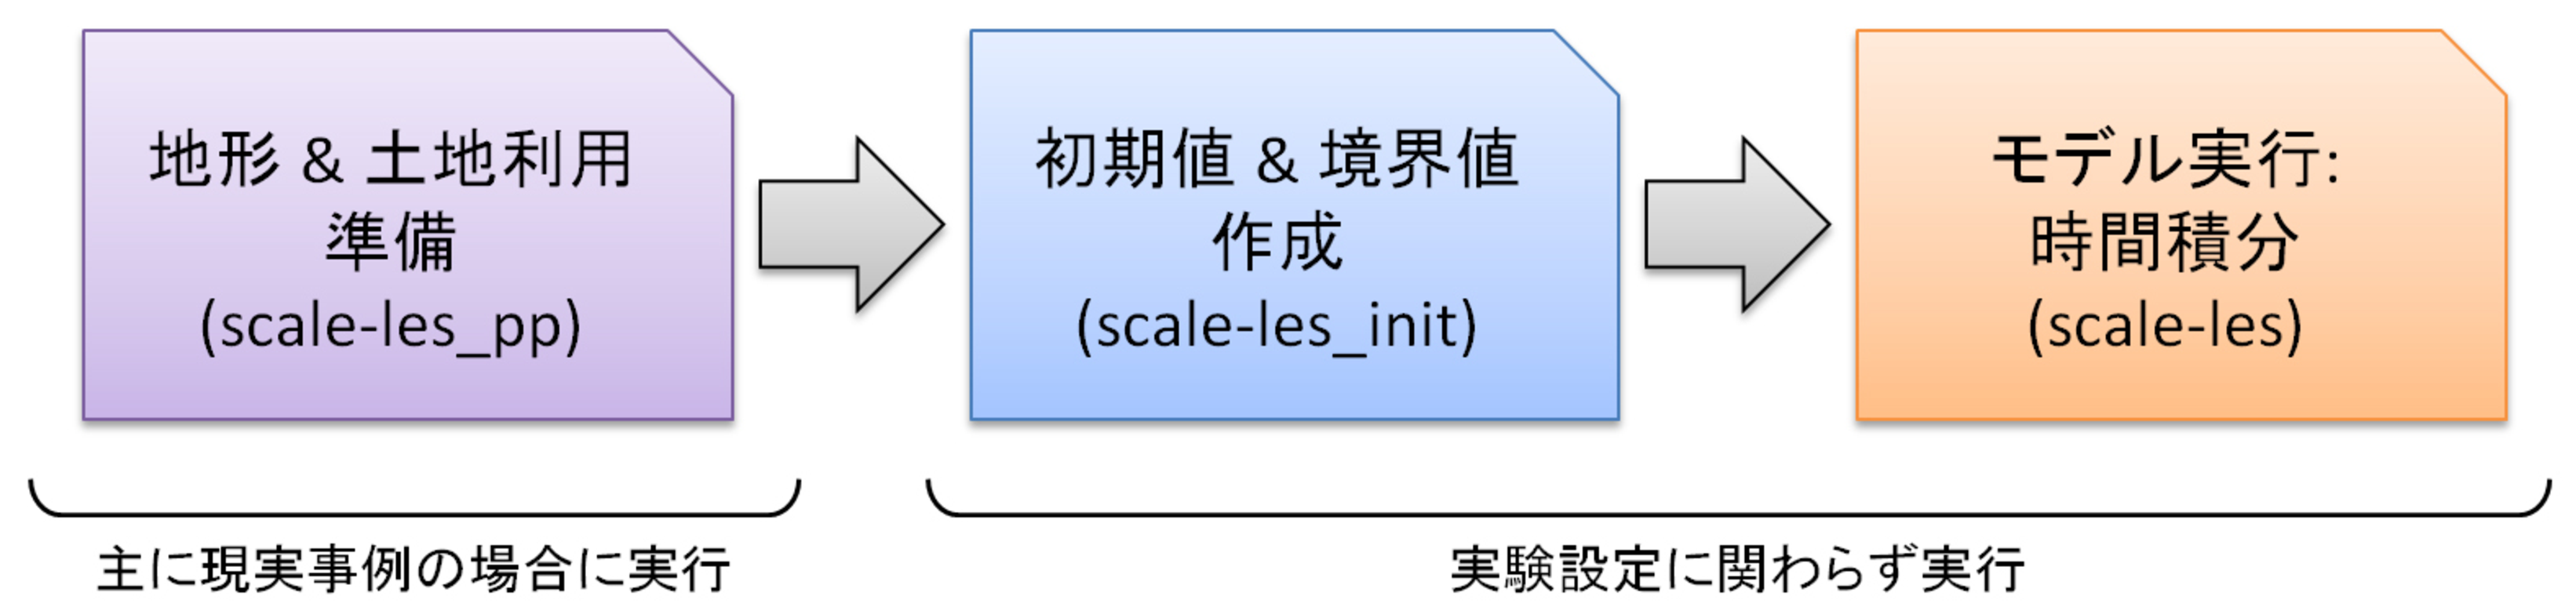
\includegraphics[width=0.9\hsize]{./figure/how_to_run.eps}\\
  \caption{SCALE-LESモデルの実行過程}
  \label{fig:howto}
\end{center}
\end{figure}

計算領域(ドメイン)の設定はTable \ref{tab:grids}のようになっている。
チュートリアルは、SCALEの使い方を学ぶことが目的であり、
短い時間で実行可能な設定にしている。
領域モデルの実験設定として必ずしも適切な設定を選択しているとは限らないので
(例えば、15kmの水平解像度で積雲パラメタリゼーションなし)
ご留意頂きたい。

このチュートリアルを実行するには、下記の条件を満たす計算機環境が必要である。
\begin{itemize}
\item CPU: 2コア/4スレッド以上の演算コアを持つCPU(4コア以上を推奨)
\item Memory容量: 4GB以上をプログラムに割当可能(8GB以上を搭載した計算機を推奨)
\item HDD空き容量: 7GB以上の空き容量
\end{itemize}
本節の説明で使用した環境は次のとおりである。
\begin{itemize}
\item CPU: Intel Xeon E5-2620 2.0GHz 6コア(ただし4コアのみ使用)
\item Memory: DDR3-1333 (4 channel, 32GB搭載)
\item OS: CentOS 6.6 x86-64, CentOS 7.1 x86-64, openSUSE 13.2 x86-64
\end{itemize}

\begin{figure}[tb]
\begin{center}
  \includegraphics[width=0.5\hsize]{./figure/real_domain.eps}\\
  \caption{計算領域.カラーシェードは地形の標高を示す.}
  \label{fig:domain}
\end{center}
\end{figure}

\begin{table}[h]
\begin{center}
  \caption{実験設定の概略}
  \label{tab:grids}
  \begin{tabularx}{150mm}{|l|X|} \hline
    \rowcolor[gray]{0.9} 項目 & 設定 \\ \hline
    MPIプロセス分割 (東西 x 南北) & 2 x 2 (合計4プロセス) \\ \hline
    水平格子数 (東西 x 南北) & 60格子点 x 60格子点 \\ \hline
    鉛直層数                 & 36層                  \\ \hline
    水平格子間隔             & dx = dy = 15km       \\ \hline
    積分期間 & 2014年8月10日 00UTC~12UTC (12時間積分) \\ \hline
    時間ステップ間隔 & 60 sec (720 steps) \\ \hline
  \end{tabularx}
\end{center}
\end{table}


%-------------------------------------------------------%
\section{境界データの準備}
%-------------------------------------------------------%

現実大気実験のシミュレーションを行う場合、SCALE本体に加えて
境界値データが必要になる。境界値データとしては下記が必要である。
{\color{blue}青字}は必須の変数、その他は任意である。

\begin{itemize}
\item 地形データ(SCALEモデルの地形を準備する)
 \begin{itemize}
  \item {\color{blue}標高データ}
  \item {\color{blue}土地利用データ}
 \end{itemize}
\item 初期値境界値データ
 \begin{itemize}
   \item {\color{blue}親モデルの緯度・経度}
   \item 3次元大気データ
     \begin{itemize}
       \item {\color{blue}東西風速, 南北風速, 気温, 比湿(相対湿度), 気圧, ジオポテンシャル高度}
     \end{itemize}
   \item 2次元大気データ
     \begin{itemize}
       \item 海面更正気圧, 地上気圧, 10m東西風速, 10m南北風速, 2m気温, 2m比湿(相対湿度)
     \end{itemize}
   \item 2次元陸面データ
     \begin{itemize}
       \item 親モデルの海陸マップ
       \item {\color{blue}地表面温度}
       \item {\color{blue}土壌データの深さ情報, 土壌温度}, 土壌水分(体積含水率 or 飽和度)
     \end{itemize}
   \item 2次元海面データ 海面水温
 \end{itemize}
\end{itemize}


\subsubsection{地形データと土地利用データ}
標高データと土地利用データは実験設定に従って、
SCALEのそれぞれの格子点における地形、海陸分布、土地利用を
作成するために使用する。
ユーザーが全球の任意の地域を対象とした計算ができるよう、
フォーマット変換済みの
標高データ USGS(U.S. Geological Survey) のGTOPO30 と、
土地利用データ GLCCv2、
を提供している。

\begin{enumerate}
\item データのダウンロード\\
SCALE用の地形・土地利用のデータを\\
 \url{http://scale.aics.riken.jp/download/scale_database.tar.gz}\\
より入手し、任意のディレクトリに展開しておく。
\begin{verbatim}
  $ tar -zxvf scale_database.tar.gz
\end{verbatim}
展開したディレクトリには、地形データと土地利用データが格納されている。
\begin{verbatim}
  scale_database/topo/    <- 地形データ
  scale_database/landuse/ <- 土地利用データ
\end{verbatim}

\item パスの設定\\
makeを使ったjob scriptを使用する場合には、
展開先のディレクトリを \verb|SCALE_DB| という環境変数に設定しておくと便利である
(以後、\verb|${SCALE_DB}|と表記)。
\begin{verbatim}
  $ export SCALE_DB=${path_to_directory_of_scale_database}/scale_database
\end{verbatim}
\end{enumerate}

\subsubsection{大気・陸面・海面水温データ}
\label{sec:real_prep}
初期値境界値データは4-byte バイナリー(grads format)に変換すれば、
任意のデータを読み込むことが可能である。
チュートリアルではNCEP FNL(Final) Operational Global Analysis dataを使用する。
\begin{enumerate}
\item データのダウンロード\\
NCARのサイト
 \url{http://rda.ucar.edu/datasets/ds083.2/}\\
から、2014年8月10日のgrib2フォーマットのデータ
\begin{verbatim}
  fnl_20140810_00_00.grib2
  fnl_20140810_06_00.grib2
  fnl_20140810_12_00.grib2
  fnl_20140810_18_00.grib2
\end{verbatim}
を\verb|${Tutrial_DIR}/real/tools/|の下にダウンロードする。

\item データフォーマットをgribからbinaryに変換\\
 SCALEは4byte バイナリー(grads format)の境界値データを読み込むことができる。\\
\verb|${Tutrial_DIR}/real/tools/| の中にある \verb|convert_grib2grads.sh|を実行。
ただし、あらかじめ\verb|wgrib2|がインストールされている必要がある.
\begin{verbatim}
  $ sh convert_grib2grads.sh
\end{verbatim}
成功すれば、下記のファイルが作成される。
\begin{verbatim}
  $ ls FNL_output/*/*
     FNL_output/201408/FNLatm_2014081000.grd
     FNL_output/201408/FNLatm_2014081006.grd
     FNL_output/201408/FNLatm_2014081012.grd
     FNL_output/201408/FNLatm_2014081018.grd
     FNL_output/201408/FNLland_2014081000.grd
     FNL_output/201408/FNLland_2014081006.grd
     FNL_output/201408/FNLland_2014081012.grd
     FNL_output/201408/FNLland_2014081018.grd
     FNL_output/201408/FNLsfc_2014081000.grd
     FNL_output/201408/FNLsfc_2014081006.grd
     FNL_output/201408/FNLsfc_2014081012.grd
     FNL_output/201408/FNLsfc_2014081018.grd
\end{verbatim}
\end{enumerate}



%-------------------------------------------------------%
\section{地形・土地利用データの作成:pp}
%-------------------------------------------------------%

ここでは,\ref{sec:source_code}節でダウンロードした\verb|tutorial_data|は,
\verb|${TOPDIR}/data/|の下に展開されていると想定している.

まず,ppディレクトリへ移動する.
ppでは現実実験のための地形データ、土地利用データを作成する.
\begin{verbatim}
 $ cd scale/scale-les/test/tutorial/pp
\end{verbatim}
ppディレクトリの中には,\verb|pp.conf|という名前の
コンフィグファイルが準備されている.
地球上でのドメインの位置や格子点数など、実験設定に合わせて,
適宜\verb|pp.conf|を編集する必要があるが,
チュートリアルでは,すでに編集済みの\verb|pp.conf|が
与えられているためそのまま利用する.
\verb|pp.conf|の設定の中で特に注意するべき項目は,\verb|PARAM_CONVERT|である.
\begin{verbatim}
 &PARAM_CONVERT
  CONVERT_TOPO = .true.,
  CONVERT_LANDUSE = .true.,
 /
\end{verbatim}
上記のように\verb|CONVERT_TOPO|と\verb|CONVERT_LANDUSE|が
\verb|.true.|となっていることが,
それぞれ地形と土地利用の処理を行うことを意味している.
詳細なコンフィグファイルの内容については,
Appendix \ref{app:namelist}を参照されたい.

次に,コンパイル済みのバイナリと入力データをppディレクトリへリンクする.
\begin{verbatim}
 $ ln -s ${TOPDIR}/bin/scale-les_pp ./
 $ ln -s ${TOPDIR}/data/tutorial_data/data/input_topo    ./
 $ ln -s ${TOPDIR}/data/tutorial_data/data/input_landuse ./
\end{verbatim}
今回は,Table \ref{tab:grids}に示されているように,
9つのMPIプロセスを使用する設定なので次のように実行する.
\begin{verbatim}
 $ mpirun -n 9 ./scale-les_pp pp.conf
\end{verbatim}
正常にジョブが終了すれば,\verb|topo_d01.pe######.nc|と\verb|landuse_d01.pe######.nc|というファイルがMPIプロセス数だけ,つまり9つずつ生成される(\verb|######|にはMPIプロセスの番号が入る).
それぞれ,ドメインの格子点に内挿された地形と土地利用の情報が入ってる.

処理内容のログとして,\verb|pp_LOG_d01.pe000000|という名前でログファイルも
出力されるので内容を確かめておくこと.
gpviewがインストールされていれば,次のコマンドによって作成された地形と土地利用データを
描画してチェックすることができる.
正しく作成されていれば,Fig. \ref{fig:domain}と同じように描かれる.
\begin{verbatim}
$ gpview topo_d01.pe00000*@TOPO --aspect=1
$ gpview landuse_d01.pe00000*@FRAC_LAND --aspect=1
\end{verbatim}





%-------------------------------------------------------%
\section{初期値・境界値データの作成:init}
%-------------------------------------------------------%

init では,SCALE計算に必要な初期値・境界値データを作成する.
まず,initディレクトリへ移動する.
\begin{verbatim}
 $ cd scale/scale-les/test/tutorial/init
\end{verbatim}

initディレクトリの中には,\verb|init.conf|という名前のコンフィグファイルが準備されている.
\verb|pp.conf|と同様に,実験設定に合わせて、この\verb|init.conf|を書き換える必要があるが、
チュートリアル用の\verb|init.conf|ファイルはTable\ref{tab:grids}の設定に
すでに合わせてある.
初期値・境界値データの作成には前節で作成した地形・土地利用データを利用する.
これは,下記のように,相対PATHを用いて参照するように設定されている.

\begin{verbatim}
&PARAM_TOPO
 TOPO_IN_BASENAME = "../pp/topo_d01",
/
&PARAM_LANDUSE
 LANDUSE_IN_BASENAME  = "../pp/landuse_d01",
/
\end{verbatim}
その他に\verb|init.conf|の設定の中で特に注意するべき項目は,
\verb|PARAM_MKINIT_REAL|である.

\begin{verbatim}
&PARAM_MKINIT_REAL
 BASENAME_BOUNDARY   = "boundary_d01",  <- 境界値データの出力名
 FILETYPE_ORG        = "NICAM-NETCDF",
 NUMBER_OF_FILES     = 2,               <- 読み込むファイルの数
 BOUNDARY_UPDATE_DT  = 21600.D0,        <- 入力データの時間間隔
 INTERP_SERC_DIV_NUM = 20,              <- 内挿計算用のチューニングパラメータ
/
\end{verbatim}

\verb|FILETYPE_ORG|は入力する気象場データのファイルフォーマットに
関するパラメータを設定しており,ここでは
NICAMモデルのnetcdf形式データのフォーマットで読み込むことを指定している.
詳細なコンフィグファイルの内容については,Appendix \ref{app:namelist}を参照されたい.

次に,コンパイル済みのバイナリをinitディレクトリへリンクする.
\begin{verbatim}
 $ ln -s ${TOPDIR}/bin/scale-les_init ./
\end{verbatim}
入力データはinitディレクトリの中に準備されている,\verb|"inputdata-link.sh"|を用いてリンクする.
\begin{verbatim}
 $ sh inputdata-link.sh
\end{verbatim}
としてスクリプトを実行することで,気象場の入力データがリンクされ,initディレクトリ内に下記のファイルがリンクされる.
このスクリプトにあるstart dateとend dateの設定項目を実験設定に対応するように編集するが、ここでは,start dateは1999/05/05 00:00:00,end dateは1999/05/06 00:00:00と設定している.もし,\verb|tutorial_data|を\verb|${TOPDIR}/data|以外の場所に展開している場合は,スクリプト内の
\verb|"dir"|の項目も適切なディレクトリに変更すること.下記ファイルにリンクが張れれば成功.
{\small
\begin{verbatim}

la_tg_00000.peall.nc    ms_qv_00000.peall.nc   oa_sst_00000.peall.nc  ss_tem_sfc_00000.peall.nc
la_tg_00001.peall.nc    ms_qv_00001.peall.nc   oa_sst_00001.peall.nc  ss_tem_sfc_00001.peall.nc
la_wg_00000.peall.nc    ms_tem_00000.peall.nc  ss_q2m_00000.peall.nc  ss_u10m_00000.peall.nc
la_wg_00001.peall.nc    ms_tem_00001.peall.nc  ss_q2m_00001.peall.nc  ss_u10m_00001.peall.nc
lsmask_00000.peall.nc   ms_u_00000.peall.nc    ss_slp_00000.peall.nc  ss_v10m_00000.peall.nc
lsmask_00001.peall.nc   ms_u_00001.peall.nc    ss_slp_00001.peall.nc  ss_v10m_00001.peall.nc
ms_pres_00000.peall.nc  ms_v_00000.peall.nc    ss_t2m_00000.peall.nc
ms_pres_00001.peall.nc  ms_v_00001.peall.nc    ss_t2m_00001.peall.nc

\end{verbatim} }

次に、陸面過程や放射過程のモデルを起動するためのパラメータファイルにリンクをはる.
\begin{verbatim}
 $ ln -s scale/scale-les/test/data/land/*  ./
 $ ln -s scale/scale-les/test/data/rad/*   ./
\end{verbatim}
上の行のリンクコマンドによって陸面過程のパラメータファイルがリンクされ,
下の行のコマンドによって放射過程のパラメータファイルがリンクされる.
準備が整ったら,9つのMPIプロセスを使用してinitを実行する.
\begin{verbatim}
 $ mpirun -n 9 ./scale-les_init init.conf
\end{verbatim}

正常にジョブが終了すれば,
\verb|boundary_d01.pe######.nc|と\verb|init_d01_00010713600.000.pe######.nc|というファイルが
MPIプロセス数だけ,つまり9つずつ生成される(\verb|######|にはMPIプロセスの番号が入る).
それぞれ,境界値データと初期値データが入ってるおり,境界値データには複数の時刻のデータが1つのファイルに含まれている.
初期値ファイルの名前のうち\verb|"00010713600.000"|の部分は,モデル内で算出された実験開始時刻を表している.

処理内容のログとして,\verb|init_LOG_d01.pe000000|という名前でログファイルも出力されるので内容を確かめておくこと.
gpviewがインストールされていれば,次のコマンドによって作成された地形と土地利用データを描画してチェックすることができる.
正しく作成されていれば,Fig. \ref{fig:init}と同じように描かれる.

\begin{verbatim}
$ gpvect --scalar --slice z=1500 --nocont --aspect=1 --range=0.001:0.015          \
         --xintv=10 --yintv=10 --unit_vect init_d01_00010713600.000.pe00*@QV      \
         init_d01_00010713600.000.pe00*@MOMX init_d01_00010713600.000.pe00*@MOMY
\end{verbatim}


\begin{figure}[h]
\begin{center}
  \includegraphics[width=0.7\hsize]{./figure/init_qv-momxy.eps}\\
  \caption{チュートリアル実験の初期場の様子:カラーシェードは高度1.5kmにおける比湿の分布,ベクトルは高度1.5kmにおける水平運動量フラックスを表している.}
  \label{fig:init}
\end{center}
\end{figure}




%-------------------------------------------------------%
\section{時間積分を行う:run}
%-------------------------------------------------------%
\subsubsection{run.confの準備}
runディレクトリへ移動する。
\begin{verbatim}
 $ cd ${Tutorial_DIR}/real/run
\end{verbatim}
%
runディレクトリの中には、\verb|run.conf|という名前の
設定ファイルが準備されており、
ドメインの位置や格子点数など、
チュートリアル用の設定(表\ref{tab:grids})に合わせて設定されている。\\

\noindent {\small {\gt
\ovalbox{
\begin{tabularx}{140mm}{l}
\verb|&PARAM_PRC| \\
\verb| PRC_NUM_X      = 2,| \\
\verb| PRC_NUM_Y      = 2,| \\
\verb| PRC_PERIODIC_X = .false.,| \\
\verb| PRC_PERIODIC_Y = .false.,| \\
\verb|/| \\
 \\
\verb|&PARAM_INDEX| \\
\verb| KMAX = 36,| \\
\verb| IMAX = 45,| \\
\verb| JMAX = 45,| \\
\verb|/| \\
\end{tabularx}
}}}\\


X方向、Y方向ともに2分割されており、
総計として4つのMPIプロセスを使用する設定となっている。
1つのMPIプロセスあたりの格子点数については、
\verb|IMAX = 45|、\verb|JMAX = 45|と指定されているため、
X方向、Y方向の総格子点数は、ともに$2 \times 45$ で90である。
計算ドメインの大きさは、
\verb|PARAM_GRID|の項目の\verb|DX|、\verb|DY|はともに20000 m(20 km)
と指定されているため、
90 個$\times$ 20 km より、1800 km $\times$ 1800 km の正方形の計算領域
が設定されていることがわかる。


モデル本体の実行には
事前に作成した地形・土地利用データや初期値・境界値データを利用する。
これらのファイルの指定は、
\verb|run.conf|の下記部分で設定する。\\

\noindent {\gt
\ovalbox{
\begin{tabularx}{140mm}{l}
\verb|&PARAM_TOPO| \\
\verb|   TOPO_IN_BASENAME = "../pp/topo_d01",| \\
\verb|/| \\
 \\
\verb|&PARAM_LANDUSE| \\
\verb|   LANDUSE_IN_BASENAME  = "../pp/landuse_d01",| \\
\verb|/| \\
 \\
\verb|&PARAM_RESTART| \\
\verb|   RESTART_OUTPUT      = .false.,| \\
\verb|   RESTART_IN_BASENAME = "../init/init_d01_20140714-180000.000",| \\
\verb|/| \\
 \\
\verb|&PARAM_ATMOS_BOUNDARY| \\
\verb|   ATMOS_BOUNDARY_TYPE        = "REAL",| \\
\verb|   ATMOS_BOUNDARY_IN_BASENAME = "../init/boundary_d01",| \\
\verb|   ATMOS_BOUNDARY_USE_VELZ    = .true.,| \\
\verb|   ATMOS_BOUNDARY_USE_QHYD    = .false.,| \\
\verb|   ATMOS_BOUNDARY_VALUE_VELZ  = 0.0D0,| \\
\verb|   ATMOS_BOUNDARY_UPDATE_DT   = 21600.0D0,| \\
\verb|/| \\
\end{tabularx}
}}\\


\verb|run.conf|の設定の中で時間積分に関する設定は、
\verb|PARAM_TIME|の項目にある。\\

\noindent {\gt\small
\ovalbox{
\begin{tabularx}{150mm}{ll}
\verb|&PARAM_TIME| & \\
\verb| TIME_STARTDATE     = 2007, 7, 14, 0, 0, 0,| &← 時間積分を開始する時刻 \\
\verb| TIME_STARTMS       = 0.D0,| &\\
\verb| TIME_DURATION      = 6.0D0,| &← 積分期間 \\
\verb| TIME_DURATION_UNIT = "HOUR",| &← \verb|TIME_DURATION|の単位\\
\verb| TIME_DT            = 90.0D0,| &← トレーサー移流計算の時間ステップ\\
\verb| TIME_DT_UNIT       = "SEC",|  &← \verb|TIME_DT|の単位\\
\verb| TIME_DT_ATMOS_DYN  = 45.0D0,| &← トレーサー移流計算以外の力学過程の時間ステップ\\
\verb| TIME_DT_ATMOS_DYN_UNIT = "SEC",| &← \verb|TIME_DT_ATMOS_DYN|の単位\\
 \\
\verb| ~~中略~~| &\\
 \\
\verb|/| &\\
\end{tabularx}
}}\\

\noindent 初期時刻\verb|TIME_STARTDATE|はUTCで指定する。
チュートリアルでは2007年7月14日18時UTCに設定している。
積分のための時間ステップは、上記の他、
それぞれの物理スキーム毎に設定できるようになっている。


計算結果の出力に関する設定は\verb|PARAM_HISTORY|で行う。\\

\noindent {\gt
\ovalbox{
\begin{tabularx}{140mm}{l}
\verb|&PARAM_HISTORY| \\
\verb|   HISTORY_DEFAULT_BASENAME  = "history_d01",|  ← 出力するファイル名\\
\verb|   HISTORY_DEFAULT_TINTERVAL = 3600.D0,|      ← 出力時間間隔\\
\verb|   HISTORY_DEFAULT_TUNIT     = "SEC",|          ← 出力時間間隔の単位\\
\verb|   HISTORY_DEFAULT_TAVERAGE  = .false.,| \\
\verb|   HISTORY_DEFAULT_DATATYPE  = "REAL4",| \\
\verb|   HISTORY_DEFAULT_ZINTERP   = .false.,|  ← 出力時に高さ面へ内挿するかどうか\\
\verb|   HISTORY_OUTPUT_STEP0      = .true.,|  ← 初期時刻(t=0)の値を出力するかどうか\\
\verb|/| \\
\end{tabularx}
}}\\

\noindent 上記の設定に従って、下記の\verb|HISTITEM|に羅列された変数が出力される。
\verb|HISTITEM|ではオプション変数を加えることで、変数毎に、出力間隔を変更したり、
平均値を出力したりすることも可能である。
これらの説明は\ref{sec:output}を参照されたい。\\

\noindent {\small {\gt
\ovalbox{
\begin{tabularx}{150mm}{l}
\verb|&HISTITEM item="DENS" /              ! density (3D)| \\
\verb|&HISTITEM item="MOMZ" /              ! vertical momentum (3D)| \\
\verb|&HISTITEM item="MOMX" /              ! horizontal momentum-x (3D)| \\
\verb|&HISTITEM item="MOMY" /              ! horizontal momentum-y (3D)| \\
\verb|&HISTITEM item="RHOT" /              ! density * potential-temperature (3D)| \\
\verb|&HISTITEM item="QV"   /               ! mixing ratio for vapor (3D)| \\
\verb|&HISTITEM item="QHYD" /              ! mixing ratio for hydrometeor (3D)| \\
\verb|&HISTITEM item="T"    /               ! temperature (3D)| \\
\verb|&HISTITEM item="PRES" /              ! pressure (3D)| \\
\verb|&HISTITEM item="U"    /               ! horizontal wind component-x (3D)| \\
\verb|&HISTITEM item="V"    /               ! horizontal wind component-y (3D)| \\
\verb|&HISTITEM item="W"    /               ! vertical wind component (3D)| \\
\verb|&HISTITEM item="PT"   /               ! potential temperature (3D)| \\
\verb|&HISTITEM item="RH"   /               ! relative humidity (3D)| \\
\verb|&HISTITEM item="PREC" /              ! precipitation (2D)| \\
\verb|&HISTITEM item="OLR"  /                ! out-going longwave radiation(2D)| \\
\verb|&HISTITEM item="U10" /                 ! horizontal wind component-x at 10m height(2D)| \\
\verb|&HISTITEM item="V10" /                 ! horizontal wind component-y at 10m height(2D)| \\
\verb|&HISTITEM item="T2"  /                ! temperature at 2m height (2D)| \\
\verb|&HISTITEM item="Q2"  /                ! mixing ratio for vapor at 2m height (2D)| \\
\verb|&HISTITEM item="SFC_PRES"   /       ! pressure at the bottom surface (2D)| \\
\verb|&HISTITEM item="SFC_TEMP"   /       ! temperature a the bottom surface (2D)| \\
\verb|&HISTITEM item="LAND_SFC_TEMP" /  ! temperature a the bottom surface for land model (2D)| \\
\verb|&HISTITEM item="URBAN_SFC_TEMP"/ ! temperature a the bottom surface for urban model (2D)| \\
\end{tabularx}
}}}\\

\noindent その他に実験で使用される物理過程の設定は、
\verb|PARAM_TRACER,PARAM_ATMOS,PARAM_OCEAN,PARAM_LAND,PARAM_URBAN|の項目に
記述されている。
詳細な設定ファイルの内容については、付録\ref{app:namelist}を参照されたい。

%
\subsubsection{実行}
コンパイル済みのバイナリをrunディレクトリへリンクする。

\begin{verbatim}
 $ ln -s ../../bin/scale-rm ./
\end{verbatim}
陸面過程や放射過程のモデルを起動するためのパラメータファイルに
リンクを張る。
\begin{verbatim}
 $ ln -s ../../../data/land/* ./   <- 陸面スキーム用のパラメータファイル
 $ ln -s ../../../data/rad/*  ./   <- 放射スキーム用のパラメータファイル
\end{verbatim}
準備が整ったら、4-MPI並列によりscale-rmを実行する。
\begin{verbatim}
  $ mpirun -n 4 ./scale-rm run.conf >& log &
\end{verbatim}


実行にはある程度時間を要するため、
上記のように標準出力をファイルへ書き出すようにして
バックグラウンドで実行すると便利である。
計算が開始されれば,処理内容のログとして、
\verb|"LOG_d01.pe000000"|が生成される。
さらに、ジョブが正常に終了すると、
\begin{verbatim}
 $ ls
  history_d01.pe000000.nc
  history_d01.pe000001.nc
  history_d01.pe000002.nc
  history_d01.pe000003.nc
\end{verbatim}
が作成される。
\verb|history_d01.pe######.nc|は
\verb|HISTITEM|に指定した出力変数が書き出される。
\verb|######|はMPIプロセス番号を表している。


%####################################################################################


\section{結果を描画する}
\label{sec:quicklook}
%####################################################################################

SCALEモデルの出力ファイルはMPIプロセス毎に出力されるため,
計算領域が分割された状態で出力される.
それぞれのファイルフォーマットは気候・予報(CF)メタデータ規約
に対応したnetcdf4形式である.
ここでは,プロセス毎に分割されたnetcdfファイルをgradsで扱うことがバイナリーファイルにまとめ、いくつか、確認のための図を示す.

\subsubsection{GrADSバイナリーに変換}
%-----------------------------------------------------------------------------------
分割されたnetcdfからGrADSバイナリー変換するには、\verb|netcdf2grads_h|を使用する.
詳細な使用方法は \ref{sec:net2g}節を参照頂きたい.

まず、\ref{sec:source_net2g}節でコンパイルしたバイナリーファイルにリンクを張る.
\begin{verbatim}
 $ ln -s ../../../../util/netcdf2grads_h/net2g ./
\end{verbatim}
ここでは例として、2次元変数であるMSLP、PRECを、
3次元変数として850hPa,500h,200hPa面のU、Vを変換する.
2次元変数のための設定は\verb|net2g.2d.conf|に、
3次元変数のための設定は\verb|net2g.3d.conf|にある.
configureの中のパラメータの設定は\ref{sec:net2g}節を参照頂きたい.

\verb|netcdf2grads_h|で使用可能なプロセス数は、
計算実行時に使用したプロセス数の約数である必要がある.
ここでは、計算に用いたのと同じ4ノード使用して変換することにする.
\begin{verbatim}
 $ mpirun -n 4 ./net2g net2g.2d.conf
 $ mpirun -n 4 ./net2g net2g.3d.conf
\end{verbatim}
成功すれば、下記のファイルが作成される.
\begin{verbatim}
  MSLP_d01z-2d.ctl
  MSLP_d01z-2d.grd
  PREC_d01z-2d.ctl
  PREC_d01z-2d.grd
  U_d01z-3d.ctl
  U_d01z-3d.grd
  V_d01z-3d.ctl
  V_d01z-3d.grd
\end{verbatim}


\subsubsection{計算結果の確認}
%-----------------------------------------------------------------------------------
現在のバージョンの\verb|netcdf2grads_h|では、
SCALEのXY格子座標でのみ、ctlファイルを作成可能である。
今後、緯度経度座標で出力できるようになる予定であるが、
作図の簡便さのために、下記の緯度経度座標で作図するためのctlを別途用意している.
\begin{verbatim}
  MSLP_d01z-2d_lcc.ctl
  PREC_d01z-2d_lcc.ctl
  U_d01z-3d_lcc.ctl
  V_d01z-3d_lcc.ctl
\end{verbatim}

計算結果確認用のサンプル図を作成するための
スクリプト\verb|checkfig.gs|を使って作図する.
\begin{verbatim}
 $ grads -blc checkfig.gs
\end{verbatim}
成功すると、下記の図が作成される.
なお、gradsのバージョンによって文法が異なるので、適宜変更する.
\begin{verbatim}
  mslp.png
  prec.png
  wind.png
\end{verbatim}
下記の図と同じであるか、答え合わせをする.

\begin{figure}[h]
\begin{center}
  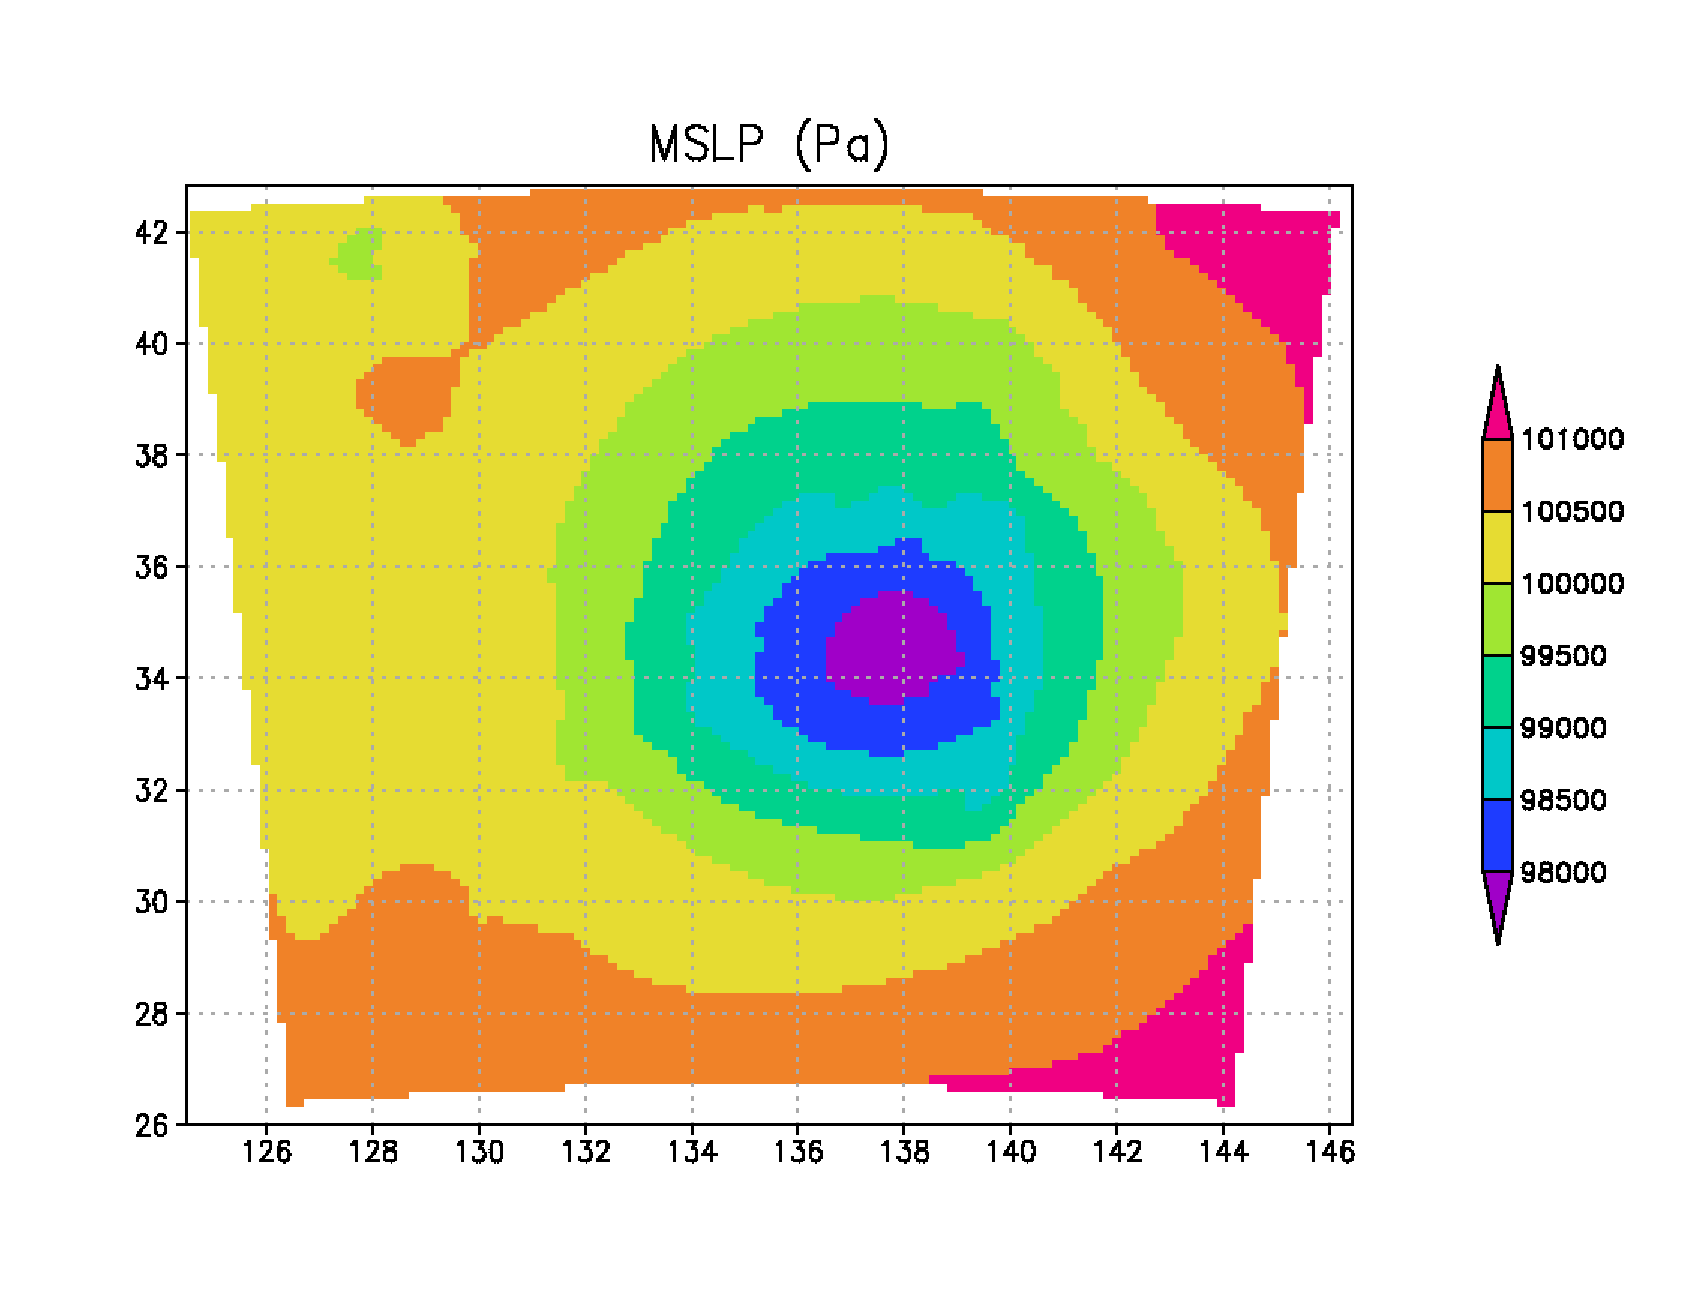
\includegraphics[width=0.55\hsize]{./figure/real_mslp.eps}\\
  \caption{計算開始から12時間後の海面更正気圧}
  \label{fig:real_mslp}
\end{center}
\begin{center}
  \includegraphics[width=0.55\hsize]{./figure/real_prec.eps}\\
  \caption{計算開始から12時間後の1時間積算降水量}
  \label{fig:real_prec}
\end{center}
\begin{center}
  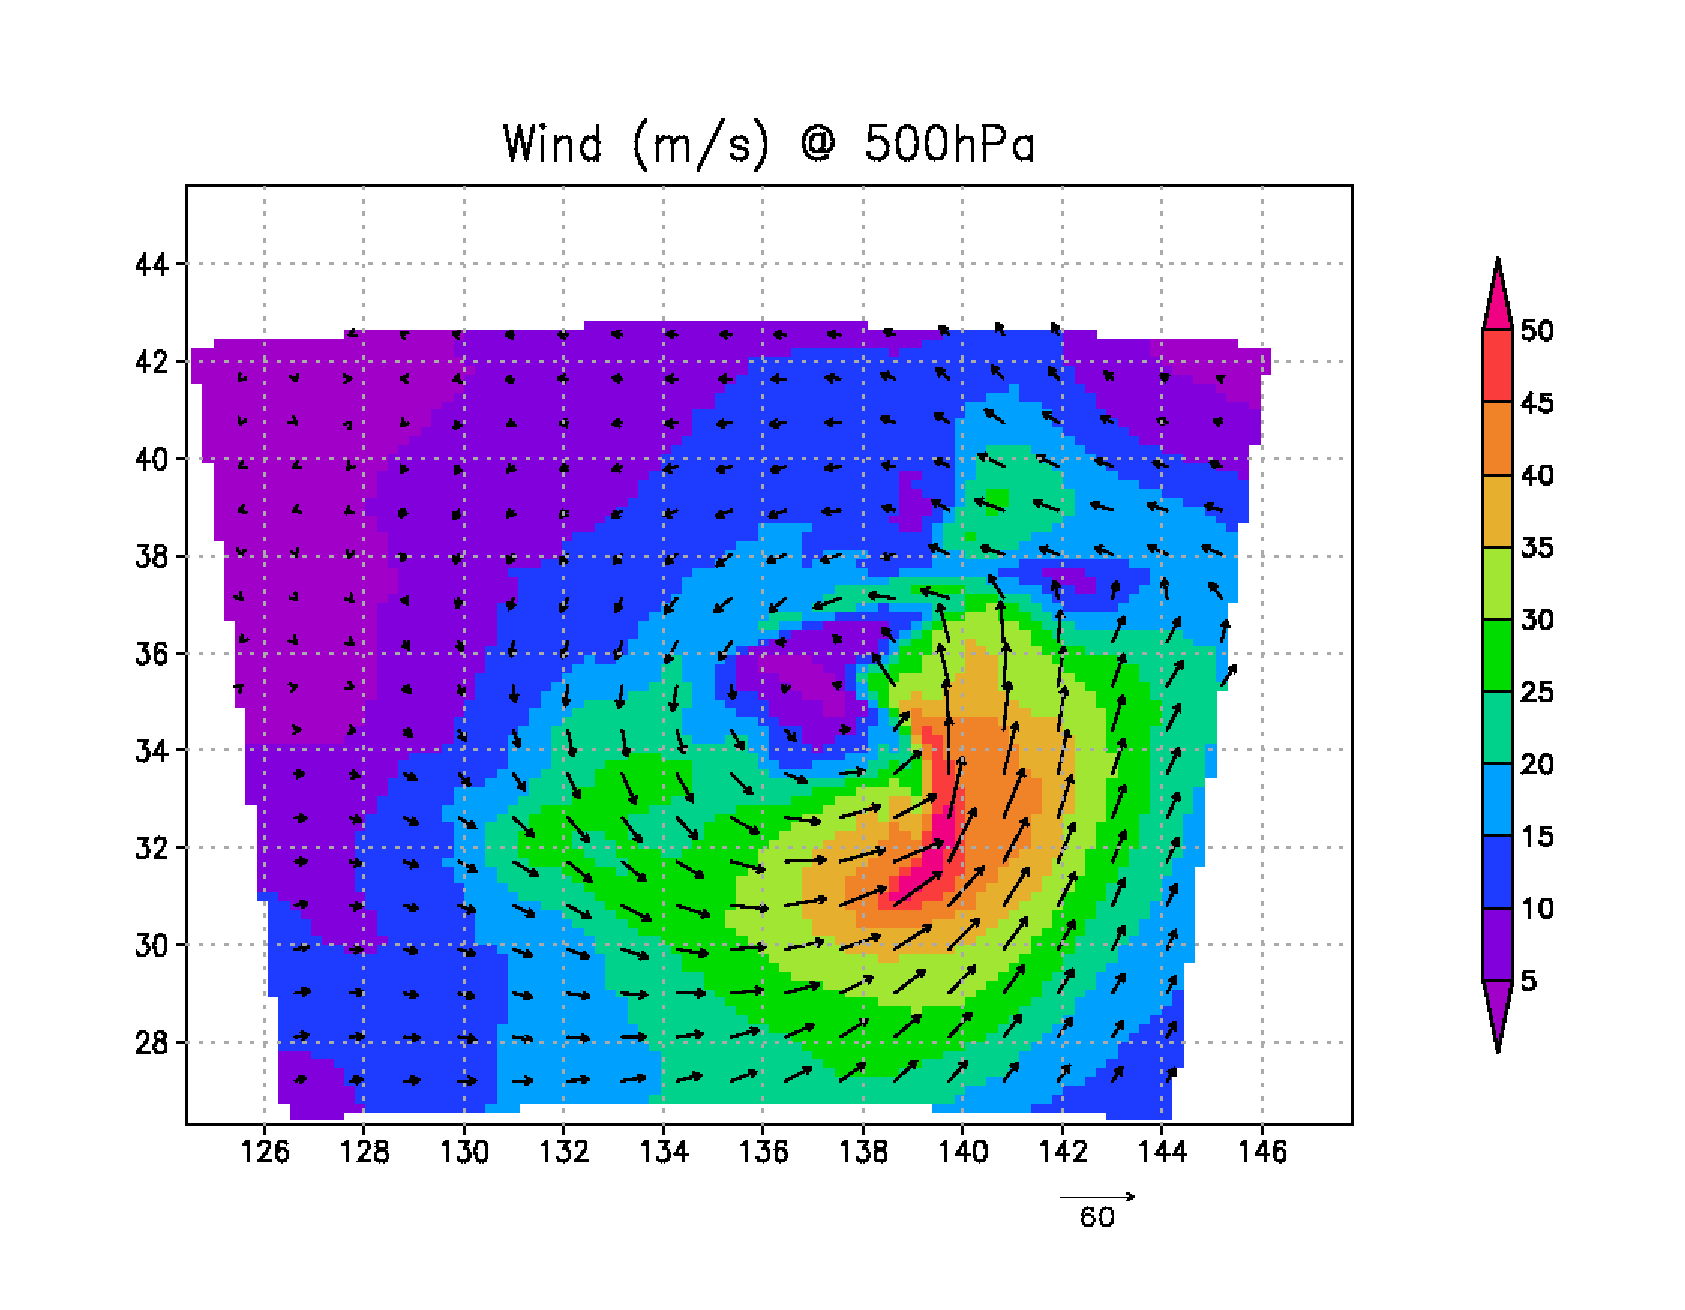
\includegraphics[width=0.55\hsize]{./figure/real_wind.eps}\\
  \caption{計算開始から12時間後の500hPaの風速と風ベクトル}
  \label{fig:real_wind}
\end{center}
\end{figure}





\chapter{各種設定: 基礎編}
\label{sec:basic}
\section{計算領域(格子数・解像度・MPIプロセス数)の指定}
\label{sec:domain}
%=======================================================================

計算領域は、水平格子間隔と格子点数を指定することで決定されるようになっている。
図\ref{fig:domain}は、
計算領域、水平格子間隔、格子数、及びMPIプロセス数の関係を示している。
水平方向に2次元の領域分割を行うことで並列化がなされている。

これらは、\namelist{PARAM_INDEX}内の\nmitem{IMAX}、\nmitem{JMAX}、
\namelist{PARAM_PRC}内の\nmitem{PRC_NUM_X}、\nmitem{PRC_NUM_Y}で
水平格子間隔については、\namelist{PARAM_GRD}内の\nmitem{DX}、\nmitem{DY}で
設定する。

ここで、注意すべきことは、「指定する格子点数は各プロセスが受け持つ値」であることである。
設定する格子数(\nmitem{IMAX}, \nmitem{JMAX}, \nmitem{KMAX})は、
1つのMPIプロセスが担当する格子点数を与える仕様となっている。
すなわち、計算領域は、水平格子間隔、格子点数とともに
各方向のMPIプロセス数を考慮して決定する必要がある。

図\ref{fig:domain}に示すように、
MPIプロセス数が$n$(=\verb|PRC_NUM_X|$\times$\verb|PRC_NUM_Y|)の時、
計算領域は、$x$方向に\verb|PRC_NUM_X|個、$y$方向に\verb|PRC_NUM_Y|個に分割される。
以上の関係から、計算領域全体のそれぞれの方向の格子点数および総格子点数は、
\begin{eqnarray}
&& x方向領域内の格子数 = \left(\verb|IMAX| \times \verb|PRC_NUM_X|\right)
   \times (\verb|KMAX| )  \nonumber\\
&& y方向領域内の格子数 = \left(\verb|JMAX| \times \verb|PRC_NUM_Y|
   \times (\verb|KMAX|\right)  \nonumber\\
&& 領域内の総格子数 = \left(\verb|IMAX| \times \verb|PRC_NUM_X|\right)
   \times (\verb|JMAX| \times \verb|PRC_NUM_Y|)
   \times (\verb|KMAX| )  \nonumber
\end{eqnarray}
の関係となる。
ここで、\verb|KMAX|は、鉛直方向の格子点数であり、
\namelist{PARAM_INDEX}内の項目で指定されている。
次節以降では、MPIプロセス数、格子数、格子間隔、
それぞれの設定方法について詳しく説明する。

\begin{figure}[h]
\begin{center}
  \includegraphics[width=0.8\hsize]{./figure/domain_decomposition.eps}\\
  \caption{計算領域に対する、水平格子間隔(DX, DY)、1MPIプロセスあたりの格子数(IMAX, JMAX)、MPIプロセス数(PRC\_NUM\_X, PRC\_NUM\_Y)の関係。
水色領域は、ある1つのMPIプロセスが担当する領域。}
  \label{fig:domain}
\end{center}
\end{figure}




\subsection{MPIプロセス数}

MPIプロセス数は、各confファイルの\verb|PARAM_PRC|で指定する。
先に述べた通り、SCALEの入出力ファイルは、MPIプロセス毎に分割されている。
そのため、MPIプロセス数を変更すると分割ファイル数も必ず変わることになる。
従って、例えば、2-MPI並列用に作成した初期値ファイルは、
4-MPI並列のモデル実行には使用できない。
MPIプロセス数を変更するには、
\verb|pp_***.conf|、\verb|init_***.conf|、\verb|run_***.conf| の
すべてを編集・変更し、\verb|pp|, \verb|init| から行う必要がある。\\

\noindent {\small {\gt
\ovalbox{
\begin{tabularx}{140mm}{lX}
\verb|&PARAM_PRC| & \\
\verb| PRC_NUM_X       = 2,| & ; X方向(東西方向)のMPI並列分割数 \\
\verb| PRC_NUM_Y       = 1,| & ; Y方向(南北方向)のMPI並列分割数 \\
\verb|/|\\
\end{tabularx}
}}}\\


全MPIプロセス数は、\verb|PRC_NUM_X| $\times$ \verb|PRC_NUM_Y|  となり、
上記の例では、X方向に2分割、Y方向に1分割(分割なし)の
2-MPI並列ということになる。

実行時にMPIコマンドに指定するMPIプロセス数は、
この総MPIプロセス数を指定しなければならない。
この条件を満たさない場合は、下記のメッセージが
LOGファイルなどに出力されて計算は行われず、直ちに終了する。

\noindent {\small {\gt
\ovalbox{
\begin{tabularx}{140mm}{l}
\verb|xxx total number of node does not match that requested. Check!| \\
\end{tabularx}
}}}\\





\subsection{水平・鉛直格子数}
%-----------------------------------------------------------------------

格子数の設定は、設定ファイル(\verb|***.conf|)の\verb|PARAM_INDEX|で行う。
以下で設定する水平格子数の値は、
1つのMPIプロセス当たりの値であることに注意が必要である。\\

\noindent {\small {\gt
\ovalbox{
\begin{tabularx}{140mm}{lX}
\verb|&PARAM_INDEX| & \\
\verb| KMAX = 97,|  & 鉛直層数 \\
\verb| IMAX = 20,|  & X方向の格子点数 \\
\verb| JMAX = 2, |  & Y方向の格子点数 \\
\verb|/|\\
\end{tabularx}
}}}\\



\subsection{水平・鉛直格子間隔}
\label{sec:gridinterv}
%-----------------------------------------------------------------------
SCALEでは、格子点の位置を均等間隔に設定することも、
任意の格子点位置を直接指定することもできる。
以下で説明する
\textcolor{red}{\bf 格子間隔の設定は、pp\_***.conf、init\_***.conf、run\_***.confの
設定ファイルの間で一致させなければならないことに注意が必要である。}
また、以下で設定する値は、MPIプロセス当たりの値であることに注意が必要である。


\subsubsection{等間隔で設定する場合}
%-----------------------------------------------------------------------&
設定ファイルの\verb|PARAM_GRID|の\verb|DX|、\verb|DY|、\verb|DZ|に
それぞれ、東西、南北、鉛直方向の格子間隔を指定する。
水平格子間隔は等間隔\footnote{緩和領域は除く(第\ref{sec:buffer}節参照)}でしか設定できない。\\

\noindent {\small {\gt
\ovalbox{
\begin{tabularx}{140mm}{lX}
\verb|&PARAM_GRID  | & \\
\verb| DX = 500.D0,| & ; X方向(東西方向)の格子間隔\\
\verb| DY = 500.D0,| & ; Y方向(南北方向)の格子間隔\\
\verb| DZ = 500.D0,| & ; Z方向(鉛直方向)の格子間隔\\
\verb|/|\\
\end{tabularx}
}}}\\


\subsubsection{任意の格子点位置を指定}
%-----------------------------------------------------------------------&
この設定方法は、鉛直方向にのみ有効である。
海面高度が0として設定されることが前提で、標高を持つ位置では山岳に沿った座標系によって適切に処理される。
SCALEの格子系は水平方向にはArakawa-Cグリッド、および鉛直方向にはLorenzグリッドである。
すなわち、速度成分定義格子点とスカラー定義格子点がスタッガード(食い違い)になっている。
スカラー量を定義している格子点をCenter Pointと呼び、半格子ズレた格子点をFace Pointと呼ぶ。
なお、これは、スカラー量のコントロールボリュームに合わせた呼称である。
SCALEでは、これらの頭文字と方向を組み合わせて
\verb|CX、CY、CZ|や\verb|FX、FY、FZ|と定義している(図\ref{fig:scale_grid})。


\begin{figure}[h]
\begin{center}
  \includegraphics[width=0.8\hsize]{./figure/Center-Face.eps}\\
  \caption{SCALE-RMの格子の定義。PARAM\_GRIDでFZを指定する時は、HALOを除いた計算領域下端の格子からk=1として与える(図b参照)。(ただし、SCALE本体では、HALOを含む領域の左下端の格子をi, j, k=1と定義している。}
  \label{fig:scale_grid}
\end{center}
\end{figure}



直接格子点の位置を指定する場合は、Z方向のFace Pointの位置を
\verb|FZ(:)|に指定
\footnote{指定の際には、シミュレーションの計算精度
(モデルのコンパイル時に指定した浮動小数点の精度。デフォルトでは倍精度)を用いることが望ましい。}
(単位はメートル[m]) すれば良い。
\verb|FZ(:)|で指定する値の数は、鉛直層数(\verb|PARAM_INDEX|の\verb|KMAX|)と一致させる必要がある。
例として理想実験のチュートリアルのrun.confファイル
(run\_R20kmDX500m.conf)を下記に示す。\\

\noindent {\small {\gt
\ovalbox{
\begin{tabularx}{140mm}{lX}
\verb|&PARAM_GRID|     & \\
\verb| DX = 500.D0,|   & X方向の格子間隔(等間隔)\\
\verb| DY = 500.D0,|   & Y方向の格子間隔(等間隔)\\
\verb| FZ(:) = |       & Z方向のFace pointの位置[m] \\
\verb|    80.000000000000000      ,| & \\
\verb|    168.00000190734863      ,| & \\
\verb|    264.80000610351567      ,| & \\
\verb|     〜 中略 〜|           & \\
\verb|    14910.428862936289      ,| & \\
\verb|    15517.262523292475      ,| & \\
\verb|    16215.121232702089      ,| & \\
\verb|    17017.658748523147      ,| & \\
\verb|    17940.576891717363      ,| & \\
\verb|    19001.932756390710      ,| & \\
\verb|    20222.492000765058      ,| & \\
\verb| BUFFER_DZ = 5000.D0,|          & 第\ref{sec:buffer}節参照\\
\verb| BUFFFACT  =   1.0D0,|          & 第\ref{sec:buffer}節参照\\
\verb|/|\\
\end{tabularx}
}}}\\


格子点位置は任意に設定できるが、場合によっては計算不安定につながる。
鉛直層の設定については、作成をサポートするツール(\verb|scale/scale-rm/util/makevgrid/|)が
用意されているので参考にされたい。
\footnote{``make\_vgrid.f90''というFortranプログラムと
いくつかのサンプルnamelistが用意されている。}
ツールをコンパイルして実行すれば直ちに設定ファイルに貼り付けて使用できる
\verb|FZ|の設定が作成される。

\section{緩和領域の設定}
\label{sec:buffer}
%-----------------------------------------------------------------------
モデル最上層での重力波の反射や現実大気実験/ネスティング実験を行う際に
側面境界で親領域と対象領域の間の不一致が起こる。
この問題を解決するため、「緩和領域」を設ける。
SCALEでは計算領域の境界のすぐ内側に緩和領域を設定することができる。
緩和領域の格子では、指定された値(境界値データ、親領域のデータなど)に対して
ある時定数で緩和される。以下これをナッジングと呼ぶ。
緩和領域の幅は、confファイルの\verb|PARAM_GRID|で設定する。
以下の設定はすべての設定ファイルにおいて共通した設定になっていなければならない。\\

\noindent {\small {\gt
\ovalbox{
\begin{tabularx}{150mm}{lX}
\verb|&PARAM_GRID  |            & \\
 \verb|BUFFER_DZ = 5000.D0,   | & ; Z方向(モデルトップから下向き方向)の緩和領域の幅 [m]\\
 \verb|BUFFER_DX = 300000.D0, | & ; X方向(東西方向)の緩和領域の幅 [m]\\
 \verb|BUFFER_DY = 300000.D0, | & ; Y方向(南北方向)の緩和領域の幅 [m]\\
 \verb|BUFFFACT  = 1.D0,      | & ; 緩和領域内の格子間隔に対するストレッチ係数(デフォルトは1.0)\\
\verb|/|\\
\end{tabularx}
}}}\\

水平方向には東西南北の四方境界に緩和領域が設定されるが、
鉛直方向には計算領域の上端にのみ緩和領域が設定され、下端には設定されない。
%
緩和領域は、計算領域内に設定されるため、
ナッジングの影響を受けない領域(緩和領域を除いた範囲)は
計算領域よりも狭くなることに注意が必要である。

\subsubsection{緩和領域の格子間隔をストレッチさせる}
緩和領域の格子間隔は、基本的に \verb|DX, DY, DZ|に指定した通りであるが、
\verb|BUFFFACT|に1以上の値を設定することで、ストレッチさせることも可能である。
この\verb|BUFFFACT|の設定は、X, Y, Z方向すべてに適用される。
ただし、\verb|PARAM_GRID|で等間隔の格子間隔を指定した場合のみ有効で、
Z方向の層レベルを任意の格子点位置に指定(\verb|FZ|を与える場合)には適用されない
(第\ref{sec:gridinterv}節参照)。

緩和領域内の格子間隔 (\verb|BDX|) は次の通り決定される。
\begin{eqnarray}
 \verb|BDX(|n\verb|)| &=& \verb|DX| \times \verb|BUFFFACT|^n \nonumber
\end{eqnarray}
ここで、$n$は緩和領域内の格子点番号を表し、計算領域の内側から外側へ向かって番号が振られる。
緩和領域の格子間隔は、
\verb|BUFFFACT=1.0|ならば内部領域と同じであり、
\verb|BUFFFACT=1.2|ならば内側から外側(境界)に向かって1.2倍の割合で広がっていく。
\verb|BUFFFACT|はいくつに設定しても良いが、計算の安定性を考慮すると 1.0から1.2 が推奨である。

緩和領域の格子数\verb|ibuff|は、$\sum_{n=1}^{\verb|ibuff|} \verb|BDX|(n) \ge$ \verb|BUFFER_DX| の関係を満たす最小の整数である。
%
緩和領域の幅(\verb|BUFFER_DX|)が同じでも、
\verb|BUFFFACT|の値を大きくすると緩和領域に用意される格子数は少なくなる。
ここでは、X方向の説明をしたが、Y方向、Z方向も同様である。


SCALEでは、緩和領域の大きさ、緩和格子点の数について、まだ明確な指標を設定できていないが、
鉛直方向(計算領域トップ)の緩和格子点は5点以上、
水平方向(側面境界付近)の緩和格子点は20〜40点程度を推奨している。
実験設定や事例によっては、さらに緩和格子点を増やしたり、
ストレッチ係数を用いて緩和領域を広げたり、
ここでは説明しないが\verb|ATMOS_BOUNDARY_taux|、\verb|ATMOS_BOUNDARY_tauy|といった項目を調整して
緩和領域のナッジング強度を調整したりする必要があるだろう。


\input{53_basic_scheme_dyn}
\section{物理スキームの設定} \label{sec:basic_physics}
%------------------------------------------------------

\subsection{雲微物理スキーム} \label{sec:basic_microphys}
%------------------------------------------------------
雲微物理スキームの選択は、init.confとrun.conf中の
\namelist{PARAM_TRACER}の中の\nmitem{TRACER_TYPE}、
及び、\namelist{PARAM_ATMOS}の\nmitem{ATMOS_PHY_MP_TYPE}で設定する。
このとき{\color{red}{\nmitem{TRACER_TYPE}と\nmitem{ATMOS_PHY_MP_TYPE}は普通は同じものを設定し}}
、かつ、\textcolor{red}{init.conf,run.confで同一の設定}とする必要がある。
ただし、\nmitem{ATMOS_PHY_MP_TYPE}を\verb|OFF|とするときは、\nmitem{TRACER_TYPE}は何を設定してもよいが、乾燥大気の計算をする場合は\verb|TRACER_TYPE = DRY|とするのがよい。
雲微物理スキームを呼び出すタイミングは、
\namelist{PARAM_TIME}で設定するが、これについては
第\ref{sec:timeintiv}節を参照のこと。
以下に、氷雲を含む1-momentバルク法を用いるときの設定を示す。


\noindent {\gt
\ovalbox{
\begin{tabularx}{140mm}{ll}
\verb|&PARAM_ATMOS  | & \\
\verb| ATMOS_PHY_MP_TYPE = "TOMITA08", | & ; 表\ref{tab:nml_atm_mp}より選択。\\
\verb|/             | & \\
\\
\verb|&PARAM_TRACER | & \\
\verb| TRACER_TYPE = "TOMITA08", | & \verb|ATMOS_PHY_MP_TYPE|と同じスキーム。\\
\verb|/             | & \\
\end{tabularx}
}}\\

\begin{table}[h]
\begin{center}
  \caption{雲微物理スキームの設定}
  \label{tab:nml_atm_mp}
  \begin{tabularx}{150mm}{lXX} \hline
    \rowcolor[gray]{0.9}  設定名 & スキームの説明 & 文献\\ \hline
     \verb|OFF|      & 雲微物理による相変化を計算しない &  \\
     \verb|KESSLER|  & 水雲のみの1-momentバルク法 & \citet{kessler_1969} \\
     \verb|TOMITA08| & 氷雲を含む1-momentバルク法 & \citet{tomita_2008} \\
     \verb|SN14|     & 氷雲を含む2-momentバルク法 & \citet{sn_2014} \\
     \verb|SUZUKI10| & 1-momentビン法(氷雲を含むか否かはオプションで選択) & \citet{suzuki_etal_2010} \\
    \hline
  \end{tabularx}
\end{center}
\end{table}

{\color{red}\verb|SUZUKI10|以外を選択する場合}は、
init.conf、run.confの\nmitem{TRACER_TYPE}と\nmitem{ATMOS_PHY_MP_TYPE}を
変更するだけで実行可能であるが、
\verb|SUZUKI10|を選択する場合は、以下のように
init.conf、run.confの双方に
下記を追加する必要がある。\\

\noindent {\gt
\ovalbox{
\begin{tabularx}{140mm}{ll}
\verb|&PARAM_BIN|   &  \\
\verb| nbin   = 33, & (ビンの数)| \\
\verb| ICEFLG =  1, & (氷雲を考慮するか否か,0->水雲のみ,1->氷雲も含む)| \\
\verb|/|            & \\
\end{tabularx}
}}\\

この場合も、
{\color{red}{init.confとrun.confに記載される\verb|PARAM_BIN|は同一にする必要がある}}。
\verb|SUZUKI10|を選択した時には、micpara.datという
雲微物理の計算に必要なファイルが自動生成される。
micpara.datがすでに存在する場合はあるものを利用するが、
nbinが変わると新たに作成しなければならない。
micpara.datの1行目にnbinの情報が記載されているが、
もしrun.confに記載されるnbinと
micpara.datに記載されているnbinが異なれば、\\

\noindent {\gt
\fbox{
\begin{tabularx}{140mm}{l}
\verb|xxx nbin in inc_tracer and nbin in micpara.dat is different check!| \\
\end{tabularx}
}}\\

\noindent というエラーメッセージを標準出力に出力して計算を行わず終了するようになっている。
そのため、nbinを変更した際は、micpara.datを消去して
新たに作り直す必要がある
(micpara.datを消して再度SCALEをSUZUKI10を用いて実行すれば自動的に新しいmicpara.datが生成される)。



\subsection{乱流スキーム} \label{sec:basic_turbulence}
%------------------------------------------------------

乱流スキームの選択は,init.confとrun.conf中の
\namelist{PARAM_ATMOS}の中の\nmitem{ATMOS_PHY_TB_TYPE}で以下のように設定する。
乱流スキームをが呼び出されるタイミングは、
\namelist{PARAM_TIME}で設定するが、これについては
第\ref{sec:timeintiv}節を参照のこと。\\

\noindent {\gt
\ovalbox{
\begin{tabularx}{140mm}{ll}
\verb|&PARAM_ATMOS  | & \\
\verb| ATMOS_PHY_TB_TYPE = "MYNN", | & ; 表\ref{tab:nml_atm_tb}より選択。\\
\verb|/             | & \\
\end{tabularx}
}}\\

\begin{table}[h]
\begin{center}
  \caption{乱流スキームの設定}
  \label{tab:nml_atm_tb}
  \begin{tabularx}{150mm}{lXX} \hline
    \rowcolor[gray]{0.9}  設定名 & スキームの説明 & 文献\\ \hline
      \verb|OFF|          & 乱流の計算を行わない &  \\
      \verb|SMAGORINSKY|  & Smagorinsky 型のサブグリッドモデル    & \citet{smagorinsky_1963,lilly_1962,Brown_etal_1994,Scotti_1993} \\
      \verb|D1980|        & Deardorff(1980)サブグリットモデル &\citet{Deardorff_1980} \\
      \verb|MYNN|         & MYNN Level 2.5 乱流モデル & \citet{my_1982,nakanishi_2004} \\
    \hline
  \end{tabularx}
\end{center}
\end{table}




\subsection{放射スキーム} \label{sec:basic_radiation}
%-------------------------------------------------------------------------------
放射スキームの選択は、init.confとrun.conf中の
\namelist{PARAM_ATMOS}の\nmitem{ATMOS_PHY_RD_TYPE}で設定する。
放射スキームが呼び出されるタイミングは、\namelist{PARAM_TIME}で以下のように設定する。
時間設定の詳細については第\ref{sec:timeintiv}節を参照のこと。\\

\noindent {\gt
\ovalbox{
\begin{tabularx}{140mm}{ll}
\verb|&PARAM_ATMOS  | & \\
\verb| ATMOS_PHY_RD_TYPE = "MSTRNX", | & ; 表\ref{tab:nml_atm_rd}より選択。\\
\verb|/             | & \\
\end{tabularx}
}}\\

\begin{table}[h]
\begin{center}
  \caption{放射スキームの選択肢}
  \label{tab:nml_atm_rd}
  \begin{tabularx}{150mm}{lXX} \hline
    \rowcolor[gray]{0.9}  設定名 & スキームの説明 & 文献\\ \hline
      \verb|OFFまたはNONE| & 放射スキームを使用しない & \\
      \verb|MSTRNX|       & mstrnX & \citet{sekiguchi_2008} \\
      \verb|WRF|          & mstrnX(長波)+Dudhia(短波) & \citet{dudhia_1989} \\
    \hline
  \end{tabularx}
\end{center}
\end{table}

放射計算のための太陽放射量は、
モデル実行の日付および時刻設定と、モデルの計算領域の緯度経度に従って計算される。
理想実験のために、太陽放射量、緯度経度、時刻を固定することも出来る。
これらは\namelist{PARAM_ATMOS_SOLARINS}で設定する。
%%%% 記載が必要!!!!!****

実験設定によっては、モデルトップの高度が10-20 kmと低いことがしばしばある。
そのため放射計算ではモデルトップとは別の最上層高度を設定し、
モデルトップより上空を何層で表現するか設定するようになっている。
放射用最上層を何kmにとるかは放射スキーム依存であるが、
例えば\verb|MSTRNX|ではデフォルトの
パラメータテーブルが想定する放射用最上層は100kmである。
追加される高度はデフォルトの場合10層で表現する。
すなわち、モデルトップが22kmであれば、放射スキーム内では
7.8km$\times$10層が追加されて計算される。
これらは\verb|MSTRNX|なら\namelist{PARAM_ATMOS_PHY_RD_MSTRN}で設定する。
%%%%% どこで?設定するのか?を記載する必要アリ

追加された層の気温・気圧プロファイルは外部から与える必要がある。
また二酸化炭素やオゾン等の気体濃度プロファイルも必要である。
SCALEでは気温・気圧についてはCIRA86
\footnote{http://catalogue.ceda.ac.uk/uuid/4996e5b2f53ce0b1f2072adadaeda262}\citep{CSR_2006}、
気体種についてはMIPAS2001\citep{Remedios_2007}の気候値を用意している。
気候値プロファイルについても、
モデル実行の日付および時刻設定とモデルの計算領域の緯度経度に従って計算される。
読み込むファイルは、
\begin{verbatim}
  scale-rm/test/data/rad/
\end{verbatim}
に用意されており、\namelist{PARAM_ATMOS_PHY_RD_PROFILE}でファイルのディレクトリと名前を指定する。
%%%%% 項目の記載が必要!!!!

\verb|MSTRNX|を実行するには、放射計算のためのパラメータテーブルが必要である。
デフォルトでは太陽放射から赤外放射までを29バンド111チャンネルに分割し、
雲・エアロゾル粒子の粒径を6ビンで表した時のテーブルを用いている。
パラメータファイル(3種類)も、
\begin{verbatim}
  scale-rm/test/data/rad/
\end{verbatim}
に用意されている。
\namelist{PARAM_ATMOS_PHY_RD_MSTRN}でファイルのディレクトリと名前を指定する。


\subsection{地表面(大気下端境界)} \label{sec:basic_surface}
%------------------------------------------------------
大気下端境界の選択は、init.confとrun.conf中の
\namelist{PARAM_ATMOS}の\nmitem{ATMOS_PHY_SF_TYPE}で以下のように設定する。
海面・陸面・都市モデルを用いない場合の
大気下端境界のフラックススキームが呼び出されるタイミングは、
\namelist{PARAM_TIME}で設定する。
時間設定の詳細については第\ref{sec:timeintiv}節を参照のこと。\\

\noindent {\gt
\ovalbox{
\begin{tabularx}{140mm}{ll}
\verb|&PARAM_ATMOS  | & \\
\verb| ATMOS_PHY_SF_TYPE = "COUPLE", | & ; 表\ref{tab:nml_atm_sf}より選択。\\
\verb|/             | & \\
\end{tabularx}
}}\\

\begin{table}[h]
\begin{center}
  \caption{大気下端境界の選択肢}
  \label{tab:nml_atm_sf}
  \begin{tabularx}{150mm}{lX} \hline
    \rowcolor[gray]{0.9}  設定名 & スキームの説明\\ \hline
      \verb|OFFまたはNONE| & 地表面フラックスを計算しない \\
      \verb|CONST|      & 地表面フラックスを任意の値に固定 \\
      \verb|BULK|       & 地表面フラックスをバルクモデルで計算 \\
      \verb|COUPLE|     & 海面・陸面・都市モデルそれぞれが計算するフラックスを受け取る \\
    \hline
  \end{tabularx}
\end{center}
\end{table}


%-------------------------------------------------------------------------------
\subsubsection{一定値設定の場合}

\nmitem{ATMOS_PHY_SF_TYPE = "CONST"}を選択した場合は、run.confで
下記を設定することにより、
任意の値に固定することが可能である。下記の値はデフォルトの設定を示す。\\

\noindent {\small {\gt
\ovalbox{
\begin{tabularx}{150mm}{lX}
 \\
 \verb|&PARAM_ATMOS_PHY_SF_CONST                | & \\
 \verb| ATMOS_PHY_SF_FLG_MOM_FLUX   =    0      | & 0: バルク係数を一定にする時 \\
                                                  &            1: 摩擦速度を一定にする時 \\
 \verb| ATMOS_PHY_SF_U_minM         =    0.0D0  | & 絶対速度の下限値 [m/s] \\
 \verb| ATMOS_PHY_SF_Const_Cm       = 0.0011D0  | & 運動量に対する一定バルク係数値 \\
                                                  &  (\verb|ATMOS_PHY_SF_FLG_MOM_FLUX = 0| のとき有効) \\
 \verb| ATMOS_PHY_SF_CM_min         = 1.0D-5    | & 運動量に対するバルク係数の下限値 \\
                                                  &  (\verb|ATMOS_PHY_SF_FLG_MOM_FLUX = 1| のとき有効) \\
 \verb| ATMOS_PHY_SF_Const_Ustar    =   0.25D0  | & 一定摩擦係数値 [m/s] \\
                                                  &  (\verb|ATMOS_PHY_SF_FLG_MOM_FLUX = 1| のとき有効) \\
 \verb| ATMOS_PHY_SF_Const_SH       =   15.0D0  | & 一定地表面顕熱フラックス値 [W/m2] \\
 \verb| ATMOS_PHY_SF_FLG_SH_DIURNAL =  .false.  | & 顕熱フラックスに日変化をつけるか否か [logical]\\
 \verb| ATMOS_PHY_SF_Const_FREQ     =   24.0D0  | & 顕熱フラックスに日変化を付けるときのサイクル [hour]\\
 \verb| ATMOS_PHY_SF_Const_LH       =  115.0D0  | & 一定地表面潜熱フラックス値 [W/m2] \\
 \verb|/|            & \\
 \\
\end{tabularx}
}}}\\

\subsubsection{バルク設定の場合}
%-------------------------------------------------------------------------------
\nmitem{ATMOS_PHY_SF_TYPE = "BULK"}を選択した場合は、
任意の地表面温度に対応したフラックスをバルクモデルに従って計算する。
これは海洋・陸面・都市モデルを用いずに下端境界を設定する際(特に理想実験)に利用される。
このとき、粗度は海面粗度の計算スキームを利用しているが、
後述するように海面粗度は定数を与えることができ、
また蒸発効率を決める係数も任意の値を設定出来るため、
海面に限定せず、陸面を想定した理想実験も行うことが出来る。

海面粗度を計算するスキームは、
run.conf中の\namelist{PARAM_ROUGHNESS}の\nmitem{ROUGHNESS_TYPE}で以下のように設定する。\\

\noindent {\gt
\ovalbox{
\begin{tabularx}{140mm}{ll}
\verb|&PARAM_ROUGHNESS  | & \\
\verb| ROUGHNESS_TYPE = "MOON07", | & ; 表\ref{tab:nml_roughness}より選択。\\
\verb|/             | & \\
\end{tabularx}
}}\\

\begin{table}[h]
\begin{center}
  \caption{海面粗度スキームの選択肢}
  \label{tab:nml_roughness}
  \begin{tabularx}{150mm}{llX} \hline
    \rowcolor[gray]{0.9}  設定名 & スキームの説明 & 文献 \\ \hline
      \verb|MOON07|   & デフォルト & \citet{moon_2007} \\
      \verb|MILLER92| &            & \citet{miller_1992} \\
      \verb|CONST|    & 定数を与える & \\
    \hline
  \end{tabularx}
\end{center}
\end{table}

また、フラックス計算に使用するバルク交換係数の計算スキームは
run.conf中の\namelist{PARAM_BULKFLUX}の\nmitem{BULKFLUX_TYPE}で以下のように設定する。\\

\noindent {\gt
\ovalbox{
\begin{tabularx}{140mm}{ll}
\verb|&PARAM_BULKFLUX  | & \\
\verb| BULKFLUX_TYPE = "B91W01", | & ; 表\ref{tab:nml_bulk}より選択。\\
\verb|/             | & \\
\end{tabularx}
}}\\

\begin{table}[h]
\begin{center}
  \caption{バルクフラックススキームの選択肢}
  \label{tab:nml_bulk}
  \begin{tabularx}{150mm}{llX} \hline
    \rowcolor[gray]{0.9}  設定名 & スキームの説明 & 文献 \\ \hline
      \verb|B91W01| & デフォルト & \citet{beljaars_1991,wilson_2001} \\
      \verb|U95|    &          & \citet{uno_1995} \\
    \hline
  \end{tabularx}
\end{center}
\end{table}



\subsection{海洋モデル} \label{sec:basic_ocean}
%-------------------------------------------------------------------------------
海洋過程は海面の状態量の更新と大気ー海洋間のフラックス計算の2つに大別される。
これらの過程を計算するタイミングはどちらも\namelist{PARAM_TIME}で設定する。
時間設定の詳細については第\ref{sec:timeintiv}節を参照のこと。\\


\subsubsection{海面スキーム}
%-------------------------------------------------------------------------------
海面の状態量(主に海面温度)の更新を担う海面スキームの選択は、init.confとrun.conf中の
\namelist{PARAM_OCEAN}の\nmitem{OCEAN_TYPE}で設定する。\\
海面のアルベドは、どの海面スキームを選択しても同じ計算スキームが適用され、
太陽天頂角に応じたアルベドが計算される。

\noindent {\gt
\ovalbox{
\begin{tabularx}{140mm}{ll}
\verb|&PARAM_OCEAN           | & \\
\verb| OCEAN_TYPE = "CONST", | & ; 表\ref{tab:nml_ocean}より選択。\\
\verb|/                      | & \\
\end{tabularx}
}}\\

\begin{table}[h]
\begin{center}
  \caption{海洋スキームの選択肢}
  \label{tab:nml_ocean}
  \begin{tabularx}{150mm}{lX} \hline
    \rowcolor[gray]{0.9}  設定名 & スキームの説明                        \\ \hline
      \verb|NONEまたはOFF|       & 土地利用にOCEANがない場合のみ使用可   \\
      \verb|CONST|               & 初期値のまま固定                      \\
      \verb|FILE|                & 外部ファイルから与える (時間変化あり) \\
      \verb|SLAB|                & スラブ海洋モデル                      \\
    \hline
  \end{tabularx}
\end{center}
\end{table}


\verb|OCEAN_TYPE = "FILE"|を選択した場合は、init.confとrun.confで外部入力ファイルの設定が必要である。
この場合、与えられた外部ファイルの空間部分布と時系列に応じて、海面温度は変化する。\\

\noindent {\gt
\ovalbox{
\begin{tabularx}{140mm}{ll}
 \verb|&EXTITEM                                  | & \\
 \verb| basename   = "../init/output/ocean_d01", | & ; 入力ファイル\\
 \verb| varname    = "OCEAN_TEMP",               | & ; \verb|"OCEAN_TEMP"|と書く。\\
 \verb| step_limit = 1800,                       | & \\
 \verb| step_fixed =  -1,                        | & \\
 \verb| enable_periodic_year  = .false.,         | & \\
 \verb| enable_periodic_month = .false.,         | & \\
 \verb| enable_periodic_day   = .false.,         | & \\
 \verb|/                                         | & \\
\end{tabularx}
}}\\


\verb|OCEAN_TYPE = "SLAB"|を選択した場合は、init.confとrun.confでスラブ混合層の深さを設定することができる。
この場合、大気-海洋間の熱フラックスの移動に応じて、スラブ混合層の温度は時間発展する。\\

\noindent {\gt
\ovalbox{
\begin{tabularx}{140mm}{ll}
 \verb|&PARAM_OCEAN_PHY_SLAB            | & \\
 \verb|  OCEAN_PHY_SLAB_DEPTH = 10.0D0, | & ; デフォルト設定[m] \\
 \verb|/                                | & \\
\end{tabularx}
}}\\

\subsubsection{大気-海洋フラックス}
%-------------------------------------------------------------------------------
海面スキームで計算された大気ー海洋間フラックスを大気に反映させるには、
\namelist{PARAM_ATMOS}で\nmitem{ATMOS_PHY_SF_TYPE = "COUPLE"}とする必要がある。\\

\noindent {\gt
\ovalbox{
\begin{tabularx}{140mm}{ll}
\verb|&PARAM_ATMOS  | & \\
\verb| ATMOS_PHY_SF_TYPE = "COUPLE", | &\\
\verb|/             | & \\
\end{tabularx}
}}\\

大気ー海洋間フラックスは、複数あるバルクスキームのいずれかを用いて計算される。
また、バルクスキーム内で利用される海面粗度長計算についても、複数のスキームが選択できる。\\

海面粗度を計算するスキームは、
run.conf中の\namelist{PARAM_ROUGHNESS}の\nmitem{ROUGHNESS_TYPE}で設定する。

フラックス計算に使用するバルク交換係数の計算スキームは
run.conf中の\namelist{PARAM_BULKFLUX}の\nmitem{BULKFLUX_TYPE}で設定する。
これらの詳細については、第\ref{sec:basic_surface}節参照のこと。



\subsection{陸面モデル} \label{sec:basic_land}
%-------------------------------------------------------------------------------
陸面過程についても、海洋過程と同じく陸面の状態量の更新と大気ー陸面間のフラックス計算の2つに大別される。
これらの過程が呼び出されるタイミングはどちらも\namelist{PARAM_TIME}で設定する。
時間設定の詳細については第\ref{sec:timeintiv}節を参照のこと。\\


\subsubsection{陸面スキーム}
%-------------------------------------------------------------------------------
陸面の状態量(主に陸面温度と土壌温度、土壌水分量)の更新を担う陸面スキームの選択は、
init.confとrun.conf中の\namelist{PARAM_LAND}の\nmitem{LAND_TYPE}で以下のように設定する。\\

\noindent {\gt
\ovalbox{
\begin{tabularx}{140mm}{ll}
\verb|&PARAM_LAND  | & \\
\verb| LAND_TYPE = "SLAB", | & ; 表\ref{tab:nml_land}より選択。\\
\verb|/             | & \\
\end{tabularx}
}}\\

\begin{table}[h]
\begin{center}
  \caption{陸面スキームの選択肢}
  \label{tab:nml_land}
  \begin{tabularx}{150mm}{llX} \hline
    \rowcolor[gray]{0.9}  設定名 & スキームの説明 \\ \hline
      \verb|NONEまたはOFF| & 土地利用にLANDがない場合のみ使用可            \\
      \verb|SLAB|         & 熱拡散モデル+バケツモデル                    \\
      \verb|CONST|        & SLABで土壌温度、土壌水分量、陸面温度を更新しない \\
    \hline
  \end{tabularx}
\end{center}
\end{table}


\nmitem{LAND_TYPE = "SLAB"}または\nmitem{LAND_TYPE = "CONST"}を選択した場合は、
土地利用区分に応じたアルベド、粗度長等のパラメータテーブルと、土地利用区分分布の入力が必要である。
パラメータテーブルは、
\begin{verbatim}
  scale-rm/test/data/land/param.bucket.conf
\end{verbatim}
に用意されている。\\


\subsubsection{大気-陸面フラックス}
%-------------------------------------------------------------------------------
陸面スキームで計算された大気ー陸面間フラックスを大気に反映させるには、
\namelist{PARAM_ATMOS}で\nmitem{ATMOS_PHY_SF_TYPE = "COUPLE"}とする必要がある。\\

\noindent {\gt
\ovalbox{
\begin{tabularx}{140mm}{ll}
\verb|&PARAM_ATMOS  | & \\
\verb| ATMOS_PHY_SF_TYPE = "COUPLE", | &\\
\verb|/             | & \\
\end{tabularx}
}}\\

大気ー陸面間フラックスの計算スキームは、陸面スキームに対応して選択される。
\nmitem{LAND_TYPE = "SLAB"}または\nmitem{LAND_TYPE = "CONST"}を選択した場合は、
海面または理想実験用の地表面で用いられるバルクスキームと同じものが利用される。\\

この時のフラックス計算に使用するバルク交換係数の計算スキームは
run.conf中の\namelist{PARAM_BULKFLUX}の\nmitem{BULKFLUX_TYPE}で設定する。\\
%%%% 記載必要


\subsection{都市モデル(大気-都市面フラックス)} \label{sec:basic_urban}
%------------------------------------------------------
都市モデルを用いる場合、
\namelist{PARAM_ATMOS}において、\nmitem{ATMOS_PHY_SF_TYPE = "COUPLE"}である必要がある。
都市モデルの選択は、init.confとrun.conf中の
\namelist{PARAM_URBAN}の\nmitem{URBAN_TYPE}で以下のように設定する。
都市モデルが呼び出されるタイミングは、
\namelist{PARAM_TIME}で設定するが、これについては
第\ref{sec:timeintiv}節を参照のこと。\\

\noindent {\gt
\ovalbox{
\begin{tabularx}{140mm}{ll}
\verb|&PARAM_ATMOS  | & \\
\verb| ATMOS_PHY_SF_TYPE = "COUPLE", | &\\
\verb|/             | & \\
\\
\verb|&PARAM_URBAN  | & \\
\verb| URBAN_TYPE="SLC", | & ; 表\ref{tab:nml_urban}より選択。\\
\verb|/             | & \\
\end{tabularx}
}}\\

\begin{table}[h]
\begin{center}
  \caption{都市スキームの選択肢}
  \label{tab:nml_urban}
  \begin{tabularx}{150mm}{llX} \hline
    \rowcolor[gray]{0.9}  設定名 & スキームの説明 & 文献\\ \hline
      \verb|OFF|  & 土地利用に都市がない場合のみ使用可 &   \\
      \verb|SLC|  & 単層キャノピーモデル   & \citet{kusaka_2001} \\
    \hline
  \end{tabularx}
\end{center}
\end{table}

\newpage
\section{積分時間と積分時間間隔の設定} \label{sec:timeintiv}
%------------------------------------------------------
積分時間やタイムステップは、実験の目的や設定によって適切に設定する必要がある。
空間解像度を変えた場合はそれに応じたタイムステップを設定する必要があり、
同じ解像度でも計算不安定を防ぐためにタイムステップを短くすることもある。

積分時間とタイムステップの設定は、
設定ファイル\verb|run_***.conf|の\verb|PARAM_PRC|の項目を編集することで設定できる。
この項目はモデル本体(\verb|scale-rm|)実行時のみで有効であり、初期化作成時には無効である。\\

\noindent {\small {\gt
\ovalbox{
\begin{tabularx}{140mm}{lX}
\verb|&PARAM_TIME| & \\
\verb| TIME_STARTDATE             = 2014, 8, 10, 0, 0, 0,| & 計算開始の日付:放射過程を用いる実験等で必要\\
\verb| TIME_STARTMS               = 0.D0,  | & 計算開始時刻[mili sec]\\
\verb| TIME_DURATION              = 12.0D0,| & 積分時間[単位は\verb|TIME_DURATION_UNIT|で設定]\\
\verb| TIME_DURATION_UNIT         = "HOUR",| & \verb|TIME_DURATION|の単位\\
\verb| TIME_DT                    = 60.0D0,| & トレーサー移流のタイムステップ\\
\verb| TIME_DT_UNIT               = "SEC", | & \verb|TIME_DT|の単位 \\
\verb| TIME_DT_ATMOS_DYN          = 30.0D0,| & 力学過程計算のタイムステップ\\
\verb| TIME_DT_ATMOS_DYN_UNIT     = "SEC", | & \verb|TIME_DT_ATMOS_DYN|の単位\\
\verb| TIME_DT_ATMOS_PHY_MP       = 60.0D0,| & 雲物理過程のタイムステップ \\
\verb| TIME_DT_ATMOS_PHY_MP_UNIT  = "SEC", | & \verb|TIME_DT_ATMOS_PHY_MP|の単位\\
\verb| TIME_DT_ATMOS_PHY_TB       = 60.0D0,| & 乱流スキームのタイムステップ \\
\verb| TIME_DT_ATMOS_PHY_TB_UNIT  = "SEC", | & \verb|TIME_DT_ATMOS_PHY_TB|の単位\\
\verb| TIME_DT_ATMOS_PHY_RD       = 600.0D0, | & 放射スキームのタイムステップ \\
\verb| TIME_DT_ATMOS_PHY_RD_UNIT  = "SEC",  | & \verb|TIME_DT_ATMOS_PHY_RD|の単位\\
\verb| TIME_DT_ATMOS_PHY_SF       = 60.0D0, | & 大気下端境界(フラックス計算)のタイムステップ\\
\verb| TIME_DT_ATMOS_PHY_SF_UNIT  = "SEC",  | & \verb|TIME_DT_ATMOS_PHY_SF|の単位\\
\verb| TIME_DT_OCEAN              = 300.0D0,| & 海面・海洋スキームのタイムステップ\\
\verb| TIME_DT_OCEAN_UNIT         = "SEC",  | & \verb|TIME_DT_OCEAN|の単位\\
\verb| TIME_DT_LAND               = 300.0D0,| & 陸面スキームのタイムステップ\\
\verb| TIME_DT_LAND_UNIT          = "SEC",  | & \verb|TIME_DT_LAND|の単位\\
\verb| TIME_DT_URBAN              = 300.0D0,| & 都市スキームのタイムステップ\\
\verb| TIME_DT_URBAN_UNIT         = "SEC",  | & \verb|TIME_DT_URBAN|の単位\\
\verb| TIME_DT_ATMOS_RESTART      = 21600.D0, | & リスタートファイル(大気)の出力間隔\\
\verb| TIME_DT_ATMOS_RESTART_UNIT = "SEC",    | & \verb|TIME_DT_ATMOS_RESTART|の単位\\
\verb| TIME_DT_OCEAN_RESTART      = 21600.D0, | & リスタートファイル(海洋)の出力間隔\\
\verb| TIME_DT_OCEAN_RESTART_UNIT = "SEC",    | & \verb|TIME_DT_OCEAN_RESTART|の単位\\
\verb| TIME_DT_LAND_RESTART       = 21600.D0, | & リスタートファイル(陸面)の出力間隔\\
\verb| TIME_DT_LAND_RESTART_UNIT  = "SEC",    | & \verb|TIME_DT_LAND_RESTART|の単位\\
\verb| TIME_DT_URBAN_RESTART      = 21600.D0, | & リスタートファイル(都市)の出力間隔\\
\verb| TIME_DT_URBAN_RESTART_UNIT = "SEC",    | & \verb|TIME_DT_URBAN_RESTART|の単位\\
\verb|/|\\
\end{tabularx}
}}}\\


\verb|TIME_DT| は、トレーサー移流のためのタイムステップであり、
格子間隔と移流速度からクーラン条件(CFL条件)を満たすように決定する。
つまり、格子間隔を移流速度で割った値が取りうる最少値よりも小さな値を設定する。
\verb|TIME_DT_ATMOS_DYN| は、力学変数の時間積分のためのタイムステップであり、音速で制約される。
計算安定性のためには、\verb|ATMOS_DYN_TINTEG_SHORT_TYPE| が \verb|RK4| の場合には
最少格子間隔(HE-VI利用時には水平の最少格子間隔)を 420 m/s で割った値が、
\verb|RK3| の場合には 840 m/s で割った値が目安となる。




\section{出力変数の追加・変更}
\label{sec:output}
%====================================================================================
新たな変数をヒストリーファイルへ追加するには、正式には次の2段階の手続きが必要である。

\begin{enumerate}
\item ソースファイルに、対象の変数をヒストリー出力するための設定をする。未設定の場合、run.confに\verb|&HISTITEM|を追加しても出力されない。
\item run.conf内の設定。各変数をヒストリーファイルに出力するかどうかを指定。コンパイルし直すことなく、実験毎に変更可能。
\end{enumerate}
主要な変数についてはすでに1の手続きは行われているため、2の手続きだけ行えばよい。
2の手続きだけで出力可能な変数については、
付録\ref{app:vari_hist}にリストアップしてあるので、そちらを参照すること。
以下では、2の手続きについて、説明する。\\

まず、出力ファイルと出力形式について、run.**.confの
\verb|&PARAM_HISTORY|に設定する。\\

\noindent {\small {\gt
\ovalbox{
\begin{tabularx}{140mm}{ll}
\verb|&PARAM_HISTORY| \\
\verb|  HISTORY_DEFAULT_BASENAME  |& \verb| = "[character]",| \\
\verb|  HISTORY_DEFAULT_TINTERVAL |& \verb| = [real],| \\
\verb|  HISTORY_DEFAULT_TUNIT     |& \verb| = "[character]",| \\
\verb|  HISTORY_DEFAULT_TAVERAGE  |& \verb| = [logical],| \\
\verb|  HISTORY_DEFAULT_ZINTERP   |& \verb| = [logical],| \\
\verb|  HISTORY_DEFAULT_DATATYPE  |& \verb| = "[character]",| \\
\verb|  HISTORY_OUTPUT_STEP0      |& \verb| = [logical],| \\
\verb|/| \\
\end{tabularx}
}}}\\

\begin{table}[htb]
\begin{center}
\caption{出力ファイルと出力形式の説明}
\begin{tabularx}{150mm}{|l|X|} \hline
 \rowcolor[gray]{0.9} 設定変数 & 説明 \\ \hline
 \verb|HISTORY_DEFAULT_BASENAME  | & 出力ファイル名。\verb|BASENAME_xxxxxx.nc|に出力される。\verb|xxxxxx|はノード番号。\\ \hline
 \verb|HISTORY_DEFAULT_TINTERVAL | & 出力の時間間隔 \\ \hline
 \verb|HISTORY_DEFAULT_TUNIT     | & \verb|HISTORY_DEFAULT_TINTERVAL|の単位\\ \hline
 \verb|HISTORY_DEFAULT_TAVERAGE  | & \verb|.false.| : 瞬間値、\verb|.true.| : 平均値。平均値の場合、
 出力タイミングの直前の\verb|HISTORY_DEFAULT_TINTERVAL|間の平均値が出力される。\\ \hline
 \verb|HISTORY_DEFAULT_DATATYPE  | & 出力値の型。``REAL4'',``REAL8''など。\\ \hline
 \verb|HISTORY_DEFAULT_ZINTERP   | & 鉛直内挿するかどうか。\verb|.false.| : モデル面出力、\verb|.true.| : Z面に内挿した値として出力。\\ \hline
 \verb|HISTORY_OUTPUT_STEP0      | & 初期時刻(t=0)の値を出力するかどうか。\verb|.true.| :出力、\verb|.false.| : 出力しない。\\ \hline
\end{tabularx}
\label{tab:history_settings}
\end{center}
\end{table}


次に、どの変数を出力するか、また各出力変数毎の出力形式の設定を、
run.**.confの\verb|HISTITEM|に追加する。
\verb|ITEM|に設定された変数が出力される。
\textcolor{blue}{青色文字}の部分はオプションで、
オプション変数が特に指定されていない場合は 
\verb|PARAM_HISTORY| 内の設定が適用される。
つまり、出力は、基本的には \verb|PARAM_HISTORY| に従って行われるが、
\verb|HISTITEM|のオプション設定をすることにより、
各変数ごとに出力形式を指定することが可能である。\\


\noindent {\small {\gt
\ovalbox{
\begin{tabularx}{140mm}{l}
\verb|&HISTITEM|\\
                 \verb| ITEM     = "[character]",| \\
\textcolor{blue}{\verb| BASENAME = "[character]",|} \\
\textcolor{blue}{\verb| TINTERVAL= [real],|} \\
\textcolor{blue}{\verb| TUNIT    = "[character]", |} \\
\textcolor{blue}{\verb| TAVERAGE = [logical],|} \\
\textcolor{blue}{\verb| ZINTERP  = [logical], |} \\
\textcolor{blue}{\verb| DATATYPE = "[character]",|} \\
\verb|/| \\
\end{tabularx}
}}}\\


\begin{table}[htb]
\begin{center}
\caption{出力ファイルと出力形式の説明}
\begin{tabularx}{150mm}{|l|X|} \hline
 \rowcolor[gray]{0.9} 設定変数 & 説明 \\ \hline
 \verb|ITEM      | & 変数名。 付録\ref{app:vari_hist}を参照\\ \hline
 \verb|BASENAME  | & \verb|HISTORY_DEFAULT_BASENAME|に同じ。ただし、変数(\verb|ITEM|)のみに適用。\\ \hline
 \verb|TINTERVAL | & \verb|HISTORY_DEFAULT_TINTERVAL|に同じ。ただし、変数(\verb|ITEM|)のみに適用。\\ \hline
 \verb|TUNIT     | & \verb|TINTERVAL|で指定した出力間隔の単位。\\ \hline
 \verb|TAVERAGE  | & \verb|HISTORY_DEFAULT_TAVERAGE|に同じ。ただし、変数(\verb|ITEM|)のみに適用。\\ \hline
 \verb|DATATYPE  | & \verb|HISTORY_DEFAULT_DATATYPE|に同じ。ただし、変数(\verb|ITEM|)のみに適用。\\ \hline
 \verb|ZINTERP   | & \verb|HISTORY_DEFAULT_ZINTERP|に同じ。ただし、変数(\verb|ITEM|)のみに適用。\\ \hline
\end{tabularx}
\label{tab:histitem}
\end{center}
\end{table}



下記に記述例を示す。
下記の設定では、\verb|history_d03.xxxxxx.nc|に4バイト実数で、
3600秒毎に\verb|HISTITEM|に指定されている変数が出力される。
ただし、``RAIN''については、600秒の出力間隔で、
前600秒の平均値として出力されることを意味している。\\

\noindent {\small {\gt
\ovalbox{
\begin{tabularx}{140mm}{l}
\verb|&PARAM_HISTORY| \\
\verb|  HISTORY_DEFAULT_BASENAME  = "history_d03",| \\
\verb|  HISTORY_DEFAULT_TINTERVAL = 3600.D0,| \\
\verb|  HISTORY_DEFAULT_TUNIT     = "SEC",| \\
\verb|  HISTORY_DEFAULT_TAVERAGE  = .false.,| \\
\verb|  HISTORY_DEFAULT_DATATYPE  = "REAL4",| \\
\verb|  HISTORY_DEFAULT_ZINTERP   = .false.,| \\
\verb|  HISTORY_OUTPUT_STEP0      = .true.,| \\
\verb|/| \\
 \\
\verb|&HISTITEM item="T"    /| \\
\verb|&HISTITEM item="PRES" /| \\
\verb|&HISTITEM item="U"    /| \\
\verb|&HISTITEM item="V"    /| \\
\verb|     〜 中略 〜|\\
\verb|&HISTITEM item="RAIN", taverage=.true., tinterval=600.D0 /| \\
\end{tabularx}
}}}\\


%%%%%%%%%%%%%%%%%%%%%%%%%%%%%%%%%%%%%%%%%%%%%%%%%%%%%%%%%%%%%%%%%%%%%%%%%%%%%%%%%%%%


\chapter{各種設定: 実用編}
\label{sec:advance}
%\section{単精度実行} \label{sec:single}
%------------------------------------------------------








\section{地図投影法と計算領域の位置} \label{sec:adv_mapproj}
%------------------------------------------------------
計算領域の位置と投影法は、configファイルの\verb|PARAM_MAPPROJ|の項目を編集することで設定できる。
\textcolor{red}{\bf この設定も、pp\_***.conf、init\_***.conf、run\_***.confのconfigファイルの間で
必ず一致させなければならない。}はじめに下記の例をもとに説明する。\\

\noindent {\small {\gt
\ovalbox{
\begin{tabularx}{140mm}{l}
\verb|&PARAM_MAPPROJ| \\
\verb| MPRJ_basepoint_lon = 138.727778D0,| \\
\verb| MPRJ_basepoint_lat = 35.360556D0,| \\
\verb| MPRJ_type          = 'MER',| \\
\verb|/| \\
\end{tabularx}
}}}\\

\noindent まず\verb|MPRJ_basepoint_lat|と\verb|MPRJ_basepoint_lon|は、計算領域の中心の緯度・経度を表す。
SCALEでは、北緯を正、南緯を負の値として表現し、経度は0度を起点に右回りで表現するため、この設定では計算領域の
中心が北緯35.360556度、東経138.727778度に位置することになる。この場所を中心に指定された大きさで、計算領域が
設定される\footnote{デフォルトではメルカトル図法に基づいて緯度・経度を計算する際の基準とする緯度は、
MPRJ\_basepoint\_latの値が使用されるが、MPRJ\_M\_latを用いて任意の緯度を指定することもできる。}。
実際にはSCALE内部での格子点は実距離に基づいて格子点が配置されるので、投影法で設定されるのは、
実距離に基づいた緯度・経度座標が計算される。この緯度・経度情報は、すべてのSCALEのNetCDF形式の出力ファイルに
含まれている。

\verb|MPRJ_type|は、地図投影法の種類を表しており、\verb|MER|はメルカトル図法を意味する。
SCALEで現在選択できる地図投影法とその指定文字列は次のとおりである。

\begin{table}[htb]
\begin{center}
\caption{SCALEで選択できる地図投影法}
\begin{tabularx}{150mm}{|l|X|} \hline
 \rowcolor[gray]{0.9} 地図投影法 & \verb|MPRJ_type| \\ \hline
 地図投影なし(理想実験用)& \verb|NONE| \\ \hline
 ランベルト正角円錐図法 & \verb|LC| \\ \hline
 極心平射図法(ポーラーステレオ) & \verb|PS| \\ \hline
 メルカトル図法 & \verb|MER| \\ \hline
 正距円筒図法 & \verb|EC| \\ \hline
\end{tabularx}
\label{tab:map_proj}
\end{center}
\end{table}

メルカトル図法以外の投影法も、\verb|MPRJ_type|の指定を変更するだけで、上記と同じように使用可能であるが、
ランベルト正角円錐図法の設定方法については、設定方法が異なるため以下で説明する。ここでは、現実大気実験
チュートリアルで使用した\verb|run.conf|ファイルを例に挙げる。\\

\noindent {\small {\gt
\ovalbox{
\begin{tabularx}{140mm}{l}
\verb|&PARAM_MAPPROJ| \\
\verb| MPRJ_basepoint_lon = 135.220404D0,| \\
\verb| MPRJ_basepoint_lat = 34.653396D0,| \\
\verb| MPRJ_type          = 'LC',| \\
\verb| MPRJ_LC_lat1       =  30.00D0,| \\
\verb| MPRJ_LC_lat2       =  40.00D0,| \\
\verb|/| \\
\end{tabularx}
}}}\\

SCALEでは``standard parallel type''の実装を採用しているため、投影を決定する上で2つの``standard latitude''の
位置を指定する必要がある。2つのstandard latitudeに挟まれた領域では、緯線・経線の長さの比が地球楕円体面上における
長さの比と近くなるように調節される。従って、メルカトル図法の場合に比べて、standard latitudeを設定する
\verb|MPRJ_LC_lat1|と\verb|MPRJ_LC_lat2|の項目が追加されている。それぞれ、南側、北側のstandard latitudeの
値を``degree''で指定する。

さらに下記のように\verb|MPRJ_basepoint_x|と\verb|MPRJ_basepoint_y|という変数を用いることで、地図投影中心と
計算領域中心をずらすこともできる。\\

\noindent {\small {\gt
\ovalbox{
\begin{tabularx}{140mm}{l}
\verb|&PARAM_MAPPROJ| \\
\verb| MPRJ_basepoint_lon = 135.220404D0,| \\
\verb| MPRJ_basepoint_lat = 34.653396D0,| \\
\verb| MPRJ_basepoint_x   = 100.0D0,| \\
\verb| MPRJ_basepoint_y   = 100.0D0,| \\
\verb| MPRJ_type          = 'LC',| \\
\verb| MPRJ_LC_lat1       =  30.00D0,| \\
\verb| MPRJ_LC_lat2       =  40.00D0,| \\
\verb|/| \\
\end{tabularx}
}}}\\

\noindent \verb|MPRJ_basepoint_x|と\verb|MPRJ_basepoint_y|は、地図投影中心の位置を、計算領域の南西端(左下角)から
の距離で指定するパラメータで、単位はメートルである。これらを指定しない場合は、デフォルト設定として計算領域中心と
地図投影中心の位置は一致する。上記の場合とデフォルト設定の場合を比較したものが図\ref{fig:map_lc}である。
図\ref{fig:map_lc}aはデフォルト設定で投影中心と計算領域中心が一致している場合、図\ref{fig:map_lc}bは、
計算領域の位置を投影中心からずらした場合の関係を表している。図\ref{fig:map_lc}bでは、計算領域の南西端から
\verb|MPRJ_basepoint_x|と\verb|MPRJ_basepoint_y|で指定した距離だけ離れた位置に投影中心がある。

\begin{figure}[t]
\begin{center}
  \includegraphics[width=0.8\hsize]{./figure/LC_latlon_xy.eps}\\
  \caption{投影中心と計算領域の関係:(a)はデフォルト設定の場合、(b)は計算領域の位置を投影中心からずらした場合。
  赤線の矩形が計算領域を表す。}
  \label{fig:map_lc}
\end{center}
\end{figure}


\section{側面境界条件} \label{sec:adv_lateralbnd}
%------------------------------------------------------
SCALEでは、側面境界条件として「周期境界条件」と「外部入力データ指定」の2種類から選択できる。デフォルトの設定は東西方向、
南北方向ともに周期境界条件となっている。主に理想実験では周期境界条件を使用し、現実大気実験では外部入力データ指定
を使用することを想定している。設定方法によっては、他の側面境界条件も設定可能であるが、現在のところ想定外の
使用方法であるためサポートできない。

側面境界条件の設定は、configファイルの\verb|PARAM_PRC|の項目を編集することで設定できる。
\textcolor{red}{\bf この設定は、pp\_***.conf、init\_***.conf、run\_***.confのconfigファイルの間で
必ず一致させなければならない。} 周期境界条件を設定したい場合は、デフォルト設定なので特にconfigファイルに記述する
必要はない。理想実験チュートリアルのconfigファイルの\verb|PARAM_PRC|の項目を見れば特に境界条件に関する記述が
ないことがわかるだろう。一方、外部入力データ指定を設定したい場合は、下記のように``\verb|PRERIODIC|''のスイッチを
``false''に指定する。\\

\noindent {\small {\gt
\ovalbox{
\begin{tabularx}{140mm}{l}
\verb|&PARAM_PRC| \\
\verb|      〜 中略 〜|\\
\verb| PRC_PERIODIC_X  = .false.,| \\
\verb| PRC_PERIODIC_Y  = .false.,| \\
\verb|/| \\
\end{tabularx}
}}}\\

\noindent 外部入力データ指定の場合は、\ref{sec:adv_gridspace}節で説明した必ず側面境界のバッファー領域を
設定しなければならない。バッファー領域でどの変数に強制をかけるか(ダンピングするか)、またその場合の時定数などの
設定はconfigファイルの\verb|PARAM_ATMOS_BOUNDARY|の項目で指定できる。現実大気実験のチュートリアルの
configファイル(\verb|run.conf|)を元にして一部の項目を説明する。\\

\noindent {\small {\gt
\ovalbox{
\begin{tabularx}{140mm}{l}
\verb|&PARAM_ATMOS_BOUNDARY|\\
\verb| ATMOS_BOUNDARY_TYPE        = "REAL",|\\
\verb| ATMOS_BOUNDARY_IN_BASENAME = "../init/boundary_d01",|\\
\verb| ATMOS_BOUNDARY_USE_VELZ    = .true.,|\\
\verb| ATMOS_BOUNDARY_USE_QHYD    = .false.,|\\
\verb| ATMOS_BOUNDARY_VALUE_VELZ  = 0.0D0,|\\
\verb| ATMOS_BOUNDARY_UPDATE_DT   = 21600.0D0,|\\
\verb|/|\\
\end{tabularx}
}}}\\

上2つの項目は、``REAL''が外部入力データを使用することを意味し、次の行の指定がその外部入力データのファイル名を指定している。
上から3つ目の設定項目である``\verb|ATMOS_BOUNDARY_USE_VELZ = .true.|''は、鉛直速度に対して「強制をかける」ことを
意味している。一方、``\verb|ATMOS_BOUNDARY_USE_QHYD = .false.|''として、凝結物の混合比に対しては逆に「強制をかけない」
設定になっている。その次の項目の``\verb| ATMOS_BOUNDARY_VALUE_VELZ|''は、鉛直速度に対して
強制をかける際、ここで指定した値、``0.0 m/s''へ近づくように強制をかけるという指定を意味する。
最後の行の``\verb|ATMOS_BOUNDARY_UPDATE_DT|''は、外部入力データの更新間隔が21600秒であることを
意味している。たとえば、6時間間隔でデータが与えられている再解析データを外部入力データとして使用する場合にこの設定になる。

他にも、水平速度東西成分(\verb|VELX|)、水平速度南北成分(\verb|VELY|)や温位(\verb|POTT|)などに対して同様の設定項目が
存在する。また、ダンピングの時定数を設定する\verb|ATMOS_BOUNDARY_TAUX|や\verb|ATMOS_BOUNDARY_TAUY|といった設定項目がある。
更なる詳細については、付録\ref{app:namelist}を参照のこと。


%と加える(どちらの変数もデフォルトはtrueで周期境界が用いられる).スポンジ層ではレイリーダンピングがかけられる.
%スポンジ層でかけるレイリーダンピングの設定はrun.confのPARAM\_ATMOS\_BOUNDARYで設定する.
%設定方法の一例とそれぞれのNamelistの意味を下に示す.
%\begin{verbatim}
% ATMOS_BOUNDARY_TYPE         = "INIT",  (初期値に近づくように緩和する)
% ATMOS_BOUNDARY_USE_VELZ     = .true., (速度の鉛直成分にダンピングを適用する)
% ATMOS_BOUNDARY_USE_VELX     = .true., (速度のx成分にダンピングを適用する)
% ATMOS_BOUNDARY_USE_VELY     = .true., (速度のy成分にダンピングを適用する)
% ATMOS_BOUNDARY_USE_POTT     = .true., (温位にダンピングを適用する)
% ATMOS_BOUNDARY_USE_QV       = .true., (温位にダンピングを適用する)
% ATMOS_BOUNDARY_TAUX         =  300.D0, (x方向のダンピングの時定数:300[sec])
% ATMOS_BOUNDARY_TAUY         =  300.D0, (y方向のダンピングの時定数:300[sec])
% ATMOS_BOUNDARY_TAUZ         =  10.D0,  (z方向のダンピングの時定数:300[sec])
%\end{verbatim}
%各Namelistの詳細はAppendixを参照されたい.



\section{任意のデータをSCALEで使用する} \label{sec:adv_datainput}
%====================================================================================

%\subsection{Topography and Landuse}

%現在のSCALEでは用意されている地形・土地利用データよりも
%高い解像度での計算ができない。
%高解像度計算のためには、ユーザーが適宜データを用意する必要がある。

%scale-rmでは日本領域については国土地理院のデータをもとにした地形,土地利用に関するデータベースを別途提供している(2.2節を参照).


\subsection{初期値・境界値データ} \label{sec:adv_bnddata}
%------------------------------------------------------
現在、SCALEでは下記のデータの読み込みとそれらに基づく初期値・境界値作成に対応している。

\begin{table}[htb]
\begin{center}
\caption{SCALEが読込に対応する外部入力データフォーマット}
\begin{tabularx}{150mm}{|l|l|X|} \hline
 \rowcolor[gray]{0.9} データ形式 & \verb|FILETYPE_ORG| & 備考 \\ \hline
 バイナリデータ & \verb|GrADS| & データ読み込み用のnamelistを別途必要とする。 \\ \hline
 NICAMデータ &  \verb|NICAM-NETCDF| & NetCDF形式のLatLonデータに対応する。 \\ \hline
 WRFデータ &  \verb|WRF-ARW| & ``wrfout''、``wrfrst''の両方に対応する。 \\ \hline
 SCALEデータ &  \verb|SCALE-RM| & historyデータのみ対応;latlonカタログを必要とする。 \\ \hline
\end{tabularx}
\label{tab:inputdata_format}
\end{center}
\end{table}

これらの使い分けは、初期値・境界値作成時、すなわち``scale-rm\_init''の実行時の設定ファイルの
\verb|PARAM_MKINIT_REAL|の項目中の\verb|FILETYPE_ORG|に表\ref{tab:inputdata_format}に示した設定値を
指定することで使い分ける。

バイナリデータとは、「4バイト単精度
浮動小数点のダイレクトアクセス方式、Fortran型バイナリデータ」を指す。その主な使用方法は、
第\ref{sec:tuto_real}章の現実大気実験チュートリアルで説明したとおりである。\textcolor{red}{GRIB/GRIB2のデータ形式は、
チュートリアルで説明した方法に基づいて、バイナリデータ形式を経由してSCALEに読み込ませることができる。}
その他に任意のデータを境界値に使用したい場合は、バイナリデータ形式に変換することで読み込ませることができる。

SCALEデータ形式は主にオフライン・ネスティング実験で使用される。詳細については、\ref{sec:nest_offline}節を
参照されたい。NICAMデータは、正20面体格子データではなく、緯度・経度座標に変換されたデータの
み読み込みに対応している。WRFデータについてはモデル出力データをそのまま使用することができる。
%これらの読み込み方法に関しては随時説明を加えていく予定。

%%%%%%%%%%%%%%%%%%%%%%%%%%%%%%%%%%%%%%%%%%%%%%%%%%%%%%%%%%%%%%%%%%%%%%%%%%%%%%%%%%%%%%

\section{ドメインネスティング実験} \label{sec:nest_exp}
%====================================================================================

本節では、SCALEでネスティング実験を行う方法について説明する。ネスティング実験とは、図\ref{fig_nestsample}に
示すように、水平格子間隔の異なる複数の計算領域(ドメイン)を設定し、領域が重複するように入れ子(ネスト)構造に
することで、広領域かつ高解像度のドメインを設定する計算領域設定方法である。図\ref{fig_nestsample}の例では、
3つのドメインを用いた3段ネスティング構成になっている。外側のドメインは比較的粗い
水平解像度であるが広い領域を取ることで大きな場の構造を表現することができる。逆に内側のドメインは、比較的狭い
領域であるが細かい水平解像度を取ることで対象とする現象の細かい構造を表現することができる。ここでは、
入れ子構造のうち、データを渡す側のドメインを「親ドメイン」、データを受ける側のドメインを「子ドメイン」と称する。

SCALEはオフライン・ネスティング実験とオンライン・ネスティング実験の両方をサポートしている。オフライン・ネスティング実験は、
はじめに親ドメインだけで時間積分を行い、その計算結果のhistoryデータを用いて、子ドメイン用の初期値・境界値を作成する。
その後に子ドメインの時間積分を行う。オンライン・ネスティング実験は、親ドメインと子ドメインを同時に実行し、適宜計算途中の
データを親ドメインから子ドメインへMPI通信によって受け渡しすることで、子ドメインの時間積分を行う。
オンライン・ネスティング実験が実行できる計算機リソースがあれば、オンラインで実行することを推奨する。
それは、オンラインの場合、子ドメインの境界条件の更新間隔は親ドメインの時間積分間隔に一致するため、
可能な限り細かい境界条件の更新間隔を得ることができる。


ドメインネスティング実験を行う上で共通する実験設定の制限事項は、基本的に以下の2点だけである。
\textcolor{red}{
\begin{itemize}
 \item 親ドメインの領域は子ドメインの領域を完全に内包しなければならない。
 \item 親ドメインの積分時間は子ドメインの積分時間を完全に内包しなければならない。
\end{itemize}
}

これに加えて、オンライン・ネスティング実験の場合、現在のところ親ドメインと子ドメインの積分時間は一致させなければならない。
SCALEではオンライン・ネスティングであっても、親ドメインと子ドメインの間で鉛直層数、鉛直層設定、地図投影法、そして
物理スキームが異なっていても構わない。

オフライン、オンラインに関わらず、ドメイン間の格子間隔比率($DX_{parent}/DX_{child}$)にシステム上は制限はないが、
この比率が大きすぎると計算結果の物理的なパフォーマンスが下がる可能性がある。本書では5倍以下で使用することを推奨する。

以降、まずは実行方法がわかりやすいオフライン・ネスティング実験から説明し、ついでオンライン・ネスティング実験に
ついて説明する。configファイルの名前に特に指定はないが、ここでの表記としては、
\textcolor{blue}{``***.parent.conf''と表記すれば、親ドメインのconfigファイルを編集する}ことを意味し、
\textcolor{blue}{``***.child.conf''と表記すれば、子ドメインのconfigファイルを編集する}ことを意味する。


\begin{figure}[t]
\begin{center}
  \includegraphics[width=1.0\hsize]{./figure/nesting_sample.eps}\\
  \caption{日本の近畿地方を対象領域としたドメインネスティング設定の例. domain 1が最外ドメインでdomain 3が最内ドメインである。
           赤い矩形と線は、それぞれの位置関係を示している。domain 1の水平格子間隔は7.5 km、domain 2は2.5 km、
           そしてdomain 3は0.5 kmである。}
  \label{fig_nestsample}
\end{center}
\end{figure}


\subsection{オフライン・ネスティング実験の方法} \label{sec:nest_offline}
%------------------------------------------------------

ここでは、親ドメインは解像度は荒いが広領域の外側ドメインで、子ドメインは領域は狭いが高解像度の内側ドメインで
あることを想定する。このとき、2段ネスティングのオフライン・ネスティング実験の実行過程は次のようになる。

{\gt
\begin{enumerate}
 \item 親ドメインの時間積分計算を行う。
 \item 親ドメインの出力ファイル(history)を用いて子ドメインの初期値/境界値を作成する。
 \item 作成した初期値/境界値を用いて子ドメインの時間積分計算を行う。
\end{enumerate}
}

以下、この流れに沿って説明を進める。親ドメインと子ドメインそれぞれについて、``pp.***.conf''、``init.***.conf''、
そして``run.***.conf''ファイルを事前に作成し、親ドメイン、子ドメインともに地形/土地利用データの作成を終え、
親ドメインについては、初期値/境界値データの作成を終えていることを想定して説明を進める。
ここで説明するオフライン・ネスティング実験の設定を記述したconfigファイルがチュートリアルディレクトリの下、
``tutorial/real/sample/offline\_nesting''に置いてあるので、説明を読み進める上で参考にしてもらいたい。

\subsubsection{親ドメインの時間積分計算を行う}
基本的には通常のシングルドメインの計算と同じ方法で実行すればよいが、``run.conf''ファイルの設定について、
次の5点の注意点・変更点がある。

\begin{itemize}
 \item 親ドメインのhistory出力間隔を適度に細かくとること。
 \item 親ドメインのhistory出力変数に必要なものが揃っているか確認すること。
 \item 親ドメインのhistory出力形式で\verb|ZINTERP|は``false''に設定すること。
 \item 親ドメインのhistory出力形式で\verb|STEP0|は``true''に設定すること。
 \item 親ドメインの計算領域を子ドメインへ伝える「カタログファイル」を出力すること。
\end{itemize}


この設定を``run.parent.conf''に適用すると下記のようになる。赤文字で示した部分が、
上記の注意点・変更点に対応する部分である。\\

\noindent {\small {\gt
\ovalbox{
\begin{tabularx}{140mm}{l}
\textcolor{red}{\verb|&PARAM_DOMAIN_CATALOGUE|} \\
\textcolor{red}{\verb| DOMAIN_CATALOGUE_OUTPUT = .true.,|} \\
\textcolor{red}{\verb|/|} \\
 \\
\verb|&PARAM_HISTORY| \\
\verb| HISTORY_DEFAULT_BASENAME  = "history",| \\
\textcolor{red}{\verb| HISTORY_DEFAULT_TINTERVAL = 600.D0,|} \\
\verb| HISTORY_DEFAULT_TUNIT     = "SEC",| \\
\verb| HISTORY_DEFAULT_TAVERAGE  = .false.,| \\
\verb| HISTORY_DEFAULT_DATATYPE  = "REAL4",| \\
\textcolor{red}{\verb| HISTORY_DEFAULT_ZINTERP   = .false.,|} \\
\textcolor{red}{\verb| HISTORY_OUTPUT_STEP0      = .true.,|} \\
\verb|/| \\
\end{tabularx}
}}}\\

\verb|PARAM_DOMAIN_CATALOGUE|の項目の``\verb|DOMAIN_CATALOGUE_OUTPUT|''の変数がカタログファイルの出力設定である。
もともとのconfigファイルには項目自体がないこともあるので、その場合は自分で項目を加えて設定すること。
カタログファイルは、``latlon\_domain\_catalogue.txt''というファイル名で出力される。この中には、MPIプロセス毎に分割
して担当した計算領域の四隅の緯度・経度が記述されている。

\verb|HISTORY_DEFAULT_TINTERVAL|の設定項目によってhistoryデータ出力間隔を指定する(単位は秒である)。指定値に
任意性はあるが、子ドメインの側面境界条件の更新間隔として使用可能であると考えられる範囲で指定すること。
親ドメイン、子ドメインの解像度、および実行環境のディスク空き容量にもよるが、おおよそ最大で1時間間隔、
出来れば10分間隔のhistoryデータ出力間隔を指定することが多い。

また、historyデータを用いて初期値/境界値データを作成するために、
下記の全ての変数を出力する必要がある。
run.confファイルの``HISTITEM''の項目を確認すること。

\begin{itemize}
 \item \verb|T2, Q2, MSLP, DENS, MOMZ, MOMX, MOMY, RHOT|
 \item \verb|QV, QC, QR, QI, QS, QG| {\small (親の雲微物理モデルに合わせて出力; 例えばTomita08なら全て)}
 \item \verb|NC, NR, NI, NS, NG| {\small (親の雲微物理モデルに合わせて出力; 例えばTomita08なら不要)}
 \item \verb|LAND_SFC_TEMP, URBAN_SFC_TEMP, OCEAN_SFC_TEMP|
 \item \verb|OCEAN_ALB_LW, OCEAN_ALB_SW, LAND_ALB_LW, LAND_ALB_SW|
 \item \verb|OCEAN_TEMP, OCEAN_SFC_Z0M, LAND_TEMP, LAND_WATER|
\end{itemize}

設定が完了すれば、``scale-rm''を実行して親ドメインの時間積分計算を行う。


\subsubsection{親ドメインの出力ファイルを用いて子ドメインの初期値/境界値を作成する}
次に計算が終わった親ドメインのhistoryデータ出力を用いて、子ドメインの初期値/境界値を作成する。
実行するプログラムは、通常の初期値/境界値作成と同じ``scale-rm\_init''だが、
``init.child.conf''を下記のように編集する。\\

\noindent {\small {\gt
\ovalbox{
\begin{tabularx}{140mm}{l}
\verb|&PARAM_MKINIT_REAL| \\
\verb| BASENAME_BOUNDARY   = "boundary",| \\
\textcolor{red}{\verb| BASENAME_ORG        = "history",|} \\
\textcolor{red}{\verb| FILETYPE_ORG        = "SCALE-RM",|} \\
\textcolor{red}{\verb| NUMBER_OF_TSTEPS    = 25,|} \\
\textcolor{red}{\verb| BOUNDARY_UPDATE_DT  = 600.D0,|} \\
\verb|/| \\
 \\
\textcolor{red}{\verb|&PARAM_NEST|} \\
\textcolor{red}{\verb| USE_NESTING               = .true.,|} \\
\textcolor{red}{\verb| OFFLINE                   = .true.,|} \\
\textcolor{red}{\verb| OFFLINE_PARENT_PRC_NUM_X  = 4,|} \\
\textcolor{red}{\verb| OFFLINE_PARENT_PRC_NUM_Y  = 4,|} \\
\textcolor{red}{\verb| OFFLINE_PARENT_KMAX       = 35,|} \\
\textcolor{red}{\verb| OFFLINE_PARENT_IMAX       = 40,|} \\
\textcolor{red}{\verb| OFFLINE_PARENT_JMAX       = 40,|} \\
\textcolor{red}{\verb| OFFLINE_PARENT_LKMAX      = 5,|} \\
\textcolor{red}{\verb| LATLON_CATALOGUE_FNAME    = "latlon_domain_catalogue.txt",|} \\
\textcolor{red}{\verb|/|} \\
\end{tabularx}
}}}\\

\noindent 読み込む外部入力データのファイル名を指定する``\verb|BASENAME_ORG|''は、親モデルのhistory.pe***.nc
ファイルを読み込むので、``history''と指定する。また、このhistoryファイルはSCALE-RMモデルの出力データなので、
``\verb|FILETYPE_ORG|''は、``SCALE-RM''と指定する。\verb|NUMBER_OF_TSTEPS|には、historyファイルが持つ時間ステップ数
を記述する(例として25が記述されているだけ)。\verb|BOUNDARY_UPDATE_DT|には、時間ステップの時間間隔を指定する
(単位は秒である)。つまり、親ドメインの\verb|HISTORY_DEFAULT_TINTERVAL|の設定項目に一致する値を指定する。
この説明では、親ドメインで600秒としたので、ここでも600秒を指定する。

\verb|PARAM_NEST|の項目は、ネスティング実験のために新たに加える項目である。もともとのconfigファイルには項目自体がないので、
自分でconfigファイルに追記する。最初の2つの項目によって、オフライン・ネスティング実験であることが決定される。
``\verb|OFFLINE_PARENT_|''で始まる6つの設定変数は、親ドメインの設定を記述する変数である。親ドメインの対応する項目を
参照して正しく設定すること。この例では、親ドメインは$4 \times 4$のMPIプロセス数を使用し、鉛直35層で、水平には1つの
MPIプロセスあたり$40 \times 40$の格子点を持っており、陸面モデルは5層モデルであることを想定している。
最後の``\verb|LATLON_CATALOGUE_FNAME|''の項目は、親ドメインを実行した時に出力したカタログファイルを指定する。

設定の編集が完了すれば、``scale-rm\_init''を実行して子ドメインの初期値/境界値を作成する。\\

\noindent {\small {\gt
\fbox{
\begin{tabularx}{140mm}{l}
\verb|xxx ERROR: REQUESTED DOMAIN IS TOO MUCH BROAD| \\
\verb|xxx -- LONGITUDINAL direction over the limit| \\
\end{tabularx}
}}}\\

\noindent 実行時に上記のようなメッセージが表示されて計算が止まる場合は、子ドメインの計算領域が親ドメインの計算領域の
外側に取られている部分がある。この場合は、各ドメインの大きさや領域中心の設定を見直す必要がある。


\subsubsection{作成した初期値/境界値を用いて子ドメインの時間積分計算を行う}
初期値/境界値作成が終われば、子ドメインの時間積分計算を実行する。子ドメインの実行は、通常の現実大気実験と何も変わらないので、
必要なデータのPATHが正しくconfigファイルに記述されていることを確認してから、``scale-rm''を実行すればよい。

1点だけ忘れやすい設定項目を挙げておく。\\

\noindent {\small {\gt
\ovalbox{
\begin{tabularx}{140mm}{l}
\verb|&PARAM_MKINIT_REAL| \\
\verb|     〜 中略 〜|\\
\textcolor{red}{\verb| BOUNDARY_UPDATE_DT  = 600.D0,|} \\
\verb|/| \\
\end{tabularx}
}}}\\

\noindent ``run.child.conf''の\verb|BOUNDARY_UPDATE_DT|を、初期値/境界値作成で使用した親ドメインの
historyデータ出力間隔に合わせておくことを忘れないようにすること。オフライン・ネスティング実験の場合、
現在のところこの設定に親ドメインと子ドメイン間で不整合あっても警告やエラーメッセージが発せられないまま、
時間積分計算が進み、場合によっては正常終了してしまうため注意が必要である。

多段のオフライン・ネスティング実験を行いたい場合は、ここまでの過程を繰り返せばよい。つまり、子ドメインとして
時間積分計算した結果を再度、親ドメインと見立てて、さらに内側の孫ドメインの初期値/境界値作成を行なえばよい。
以上でオフライン・ネスティングの実行方法の説明を終える。


\subsection{オンライン・ネスティング実験の方法} \label{sec:nest_online}
%------------------------------------------------------

オフライン・ネスティング実験では、各ドメインの計算を逐次的に実行する必要があったが、オンライン・ネスティング実験では
全てのドメインの計算を同時に実行する。現在は、親ドメインから子ドメインへのみデータ受け渡しを行う、いわゆる
``1-Wayネスティング''のみをサポートしている。オンライン・ネスティング実験でサポートするネスティング段数は、
最大で10段までである。

SCALEのオンライン・ネスティング実験は、複数のドメインを逐次的に時間積分計算を進めるのではなく、並列的に時間積分計算を行う。
図\ref{fig_mpisplit}に示すイメージ図のように、与えられたMPIプロセスを分割してそれぞれのドメインに分配し、各々のドメインが
独立したモデルのように計算を進める。後ほど説明するが、複数のドメインを立ち上げるために実行時には``launch.conf''という
起動用のconfigファイルが別途必要になる。

\begin{figure}[t]
\begin{center}
  \includegraphics[width=0.8\hsize]{./figure/mpisplit_nesting.eps}\\
  \caption{オンライン・ネスティング実験のMPIプロセス配分イメージ. 全部で13のプロセスを立ち上げ、これを適切に分配することで、
           Domain 1は$2 \times 2$の4-MPI並列、Domain 2は$3 \times 3$の9-MPI並列計算を行う。Domain 1からDomain 2へMPI通信
           によってデータを受け渡ししながら時間積分計算を進める。}
  \label{fig_mpisplit}
\end{center}
\end{figure}


ここでは、最も単純な2段ネスティングの例を説明する。親ドメインは解像度は荒いが広領域の外側ドメインで、
子ドメインは領域は狭いが高解像度の内側ドメインであることを想定する。

オンライン・ネスティング実験を行う場合は、``scale-rm''のモデル本体実行前に全てのドメインについて、
地形/土地利用データの作成、及び初期値/境界値データの作成を事前に行っておく必要がある。従って、親ドメインと子ドメイン
それぞれについて、``pp.***.conf''、``init.***.conf''、そして``run.***.conf''ファイルを事前に作成し、
親ドメイン、子ドメインともに地形/土地利用データの作成、及び初期値/境界値データの作成を終えていることを想定して説明を進める。
ここで説明するオンライン・ネスティング実験の設定を記述したconfigファイルがチュートリアルディレクトリの下、
``tutorial/real/sample/online\_nesting''に置いてあるので、説明を読み進める上で参考にしてもらいたい。


\subsubsection{configファイルの編集}
まず、親ドメイン、子ドメインそれぞれに``run.***.conf''ファイルを編集する。

\noindent {\gt \verb|run.parent.conf|の編集内容}\\
{\small {\gt
\ovalbox{
\begin{tabularx}{140mm}{l}
\verb|&PARAM_NEST| \\
\verb| USE_NESTING              = .true.,| \\
\verb| OFFLINE                  = .false.,| \\
\verb| ONLINE_DOMAIN_NUM        = 1,| \\
\verb| ONLINE_IAM_PARENT        = .true.,| \\
\verb| ONLINE_IAM_DAUGHTER      = .false.,| \\
\verb| ONLINE_BOUNDARY_USE_QHYD = .true.,| \\
\verb| ONLINE_AGGRESSIVE_COMM   = .true.,| \\
\verb|/| \\
\end{tabularx}
}}}\\

\vspace{0.5cm}

\noindent {\gt \verb|run.child.conf|の編集内容}\\
{\small {\gt
\ovalbox{
\begin{tabularx}{140mm}{l}
\verb|&PARAM_NEST| \\
\verb| USE_NESTING              = .true.,| \\
\verb| OFFLINE                  = .false.,| \\
\verb| ONLINE_DOMAIN_NUM        = 2,| \\
\verb| ONLINE_IAM_PARENT        = .false.,| \\
\verb| ONLINE_IAM_DAUGHTER      = .true.,| \\
\verb| ONLINE_BOUNDARY_USE_QHYD = .true.,| \\
\verb| ONLINE_AGGRESSIVE_COMM   = .true.,| \\
\verb|/| \\
\end{tabularx}
}}}\\

\noindent 上記の\verb|PARAM_NEST|の項目は、ネスティング実験のために新たに加える項目である。
もともとのconfigファイルには項目自体がないので、自分でconfigファイルに追記する。最初の2つの項目によって、
オンライン・ネスティング実験であることが決定される。``\verb| ONLINE_|''で始まる設定変数はオンライン・ネスティング実験
専用の設定変数である。\verb|ONLINE_DOMAIN_NUM|は、ドメインのID番号であり、外側ドメインから内側ドメインへ順番に
番号を振っていく。ここでは、親ドメインは1番、子ドメインは2番と設定する。

\verb|ONLINE_IAM_PARENT|と\verb|ONLINE_IAM_DAUGHTER|は各ドメインの役割を設定するパラメータである。
これらの変数は、``In online nesting system, I am parent (or, I am child).''という意味で覚えれば設定を間違うことはない。
少し脇道にそれるが、ここで説明している設定より複雑なものとして、図\ref{fig_nestsample}のような
3段ネスティング実験の場合の設定例を表\ref{tab:triple_nested}に示した。

\begin{table}[htb]
\begin{center}
\caption{3段ネスティング実験の設定例}
\begin{tabularx}{150mm}{|l|l|l|X|} \hline
 \rowcolor[gray]{0.9} ドメイン & \verb|ONLINE_DOMAIN_NUM| & \verb|ONLINE_IAM_PARENT| & \verb|ONLINE_IAM_CHILD|\\ \hline
 最外ドメイン & 1 & \textcolor{blue}{true} & \textcolor{red}{false} \\ \hline
 中間ドメイン & 2 & \textcolor{blue}{true} & \textcolor{blue}{true} \\ \hline
 最内ドメイン & 3 & \textcolor{red}{false} & \textcolor{blue}{true} \\ \hline
\end{tabularx}
\label{tab:triple_nested}
\end{center}
\end{table}

\noindent 最外ドメインは親ドメインとしてのみ働き、最内ドメインは子ドメインとしてのみ働く。一方、中間ドメインは最外ドメインに
対しては子ドメイン、最内ドメインに対しては親ドメインとして働くため両方共``true''となる。

さて、configファイルの編集内容の説明に戻る。\verb|ONLINE_BOUNDARY_USE_QHYD|は、「側面境界条件として親ドメインの凝結物の
混合比を使うかどうか」を指定する設定変数である。外部入力データから側面境界条件を作成するときには通常使わないが、
ネスティングの場合、ドメイン間の物理スキームの違いがなかったり、解像度もそれほど大きく離れていないため、側面境界から
凝結物自体が移流して入ってくる設定も選択肢に入るだろう。側面境界付近で雲が立ちにくい問題を解決したり、親ドメインとの乖離を
抑制したりする可能性がある。

最後の\verb|ONLINE_AGGRESSIVE_COMM|はオンライン・ネスティング時のドメイン間通信に関する最適化変数である。
通常は、``true''と設定して実行する。


\subsubsection{launchファイルの編集}
オンライン・ネスティング実験の実行には、``run.***.conf''の他に、起動用configファイル``launch.conf''が必要である。
\begin{verbatim}
 $ vi launch.conf
\end{verbatim}
などとして、適宜エディタをたちあげて新規ファイルを作成し、下記の内容を記述する。\\

\noindent {\small {\gt
\ovalbox{
\begin{tabularx}{140mm}{l}
\verb|&PARAM_LAUNCHER| \\
\verb| NUM_DOMAIN  = 2,| \\
\verb| CONF_FILES  = run.parent.conf,run.child.conf,| \\
\verb| PRC_DOMAINS = 4,9,| \\
\verb|/| \\
\end{tabularx}
}}}\\

\noindent 図\ref{fig_mpisplit}のイメージを思い浮かべながら設定を確認してもらいたい。\verb|PARAM_LAUNCHER|の項目のうち、
\verb|NUM_DOMAIN = 2|が「2つのドメインを起動する」ことを表しており、\verb|CONF_FILES|の項目に羅列されたファイル名は、
各々のドメインで読み込むconfigファイルを指定している。\verb|PRC_DOMAINS|は各々のドメインで使用するMPIプロセス数を
指定する。\verb|PRC_DOMAINS|は、\verb|CONF_FILES|で羅列した順番で指定しなければならない。従ってこの場合、
親ドメインは4-MPI並列、子ドメインは9-MPI並列で実行するように指定されている。ここで指定するMPIプロセス数は、
各々の``run.***.conf''で指定されている総MPIプロセス数と合致させなければならない。
この2段オンライン・ネスティング実験で使用する総MPIプロセス数は、$4 + 9 = 13$プロセスとなる。

実行時には、シングルドメイン計算とは異なり、\verb|launch.conf|を引数に指定し、計算全体で使用するMPIプロセス数を
指定して実行する。
\begin{verbatim}
 $ mpirun  -n  13  ./scale-rm  launch.conf
\end{verbatim}

実行にあたって注意することは、複数のドメインの計算を同時に実行するため、\textcolor{red}{ドメイン間でconfigファイルに
記述された出力ファイル名をドメイン毎に変更しなければならない}ことである。たとえば,``history.pe***.nc''は、
``history\_d01.pe***.nc''、``history\_d02.pe***.nc''といったようにドメイン毎に名前を変えながらどのドメインの
出力データであるか判別がつくようにconfigファイルの記述を設定する。
historyファイルのほかに、LOGファイル、topoファイル、landuseファイル、boundaryファイル、initファイル、restartファイル、
そしてmonitorファイルの名前を変更しておく必要がある。

実行時に次のようなエラーメッセージが出力されて計算が異常終了することがある。\\

\noindent {\small {\gt
\fbox{
\begin{tabularx}{140mm}{l}
\verb|xxx region of daughter domain is larger than that of parent: SW search| \\
\end{tabularx}
}}}\\

\noindent {\small {\gt
\fbox{
\begin{tabularx}{140mm}{l}
\verb|xxx region of daughter domain is larger than that of parent: NE search| \\
\end{tabularx}
}}}\\

\noindent これは、子ドメインで設定された計算領域が親ドメインの計算領域よりも大きいことを意味するエラーメッセージである。
``SW search''のエラーが出る場合は子ドメインの西側か南側が親ドメインの外側に出ており、``NE search''のエラーが出る場合は
子ドメインの東側か北側が親ドメインの外側に出ていることを意味している。再度設定を確認し、地形・土地利用データ、および
初期値/境界値作成からやり直すこと。


\subsubsection{MPIプロセスの分配ガイドライン}
SCALEのオンライン・ネスティング実験は、図\ref{fig_mpisplit}のイメージ図で説明したように、MPIプロセスを分割し、複数のドメイン
に分配する。現在のところ、その分配割合はユーザーに委ねられているため、適切にMPIプロセスを分配しなければ余計な計算時間が
かかってしまう。ここでは、適切にMPIプロセスを分配するためのガイドラインについて説明する。ガイドラインは、ドメイン毎に
\textcolor{blue}{「単位あたりの時間積分にかかる1プロセスあたりの演算量を揃える」}という単純なものである。
ここでは、以下に示す2段オンライン・ネスティング実験を行う場合を想定し、ガイドラインに沿ったプロセス分配方法の例を示す。
``domain 1''は外側の親ドメイン、``domain 2''は内側の子ドメインを意味する。

\begin{table}[htb]
\begin{center}
\caption{2段オンライン・ネスティング実験の設定想定}
\begin{tabularx}{150mm}{|l|l|X|} \hline
 \rowcolor[gray]{0.9} 設定項目 & domain 1 & domain 2 \\ \hline
 計算領域 & 450 km $\times$ 450 km & 200 km $\times$ 200 km \\ \hline
 DX \& DY(X,Y同一設定) & 3 km & 1 km \\ \hline
 鉛直層設定 & 40層 & 60層 \\ \hline
 積分時間間隔(DT)& 30 sec & 10 sec \\ \hline
 積分時間 & 3600 sec & 3600 sec \\ \hline
\end{tabularx}
\label{tab:nest_proc_guide1}
\end{center}
\end{table}

このとき、親ドメインの水平方向の一辺の格子点数は、$450 km \div 3 km = 150$点であるので、総格子点数は
$X \times Y \times Z = 150 \times 150 \times 40 = 900,000$点である。一方、子ドメインの水平方向の一辺の格子点数は、
$200 km \div 1 km = 200$点であるので、総格子点数は$200 \times 200 \times 60 = 2,400,000$点である。1つの時間ステップの
積分を行うのにこれだけの格子点について計算を行わなければならない。

積分時間間隔は格子間隔に依存するためにドメイン毎に異なる。この例では、domain 1は30 secだが、domain 2は10 secであり、
3倍の差がある。したがって、同じ30 secという積分時間に対してdomain 2は3倍多くの時間ステップ、つまり3倍の演算量を要する。
これらを考慮して、簡単なドメイン間の演算量比率(Computation Rate)の指標を考えると下記の式で表される。
\begin{eqnarray}
ComputationRate=\frac{Xgrd_{child} \times Ygrd_{child} \times Zgrd_{child} \times Ustep_{child}}
                     {Xgrd_{parent} \times Ygrd_{parent} \times Zgrd_{parent} \times Ustep_{parent}} \nonumber
\end{eqnarray}
ここで、Xgrd、Ygrd、ZgrdはそれぞれX方向、Y方向、Z方向の格子点数を表し、Ustepは単位時間積分に必要な時間ステップ数を表す。
ここでの例をこの式に当てはまると、演算量比率は$(2,400,000 \times 3) \div (900,000 \times 1) = 8$であることがわかる。
おおよそ、この割合にしたがってMPIプロセスをドメイン毎に分配すればよい。例えばdomain 1は4プロセス、domain 2は32プロセスを
使用し、全体で36プロセスを使用する設定が考えられる。この場合、例えば次のように設定することができる。

\begin{table}[htb]
\begin{center}
\caption{2段オンライン・ネスティング実験のMPIプロセス設定例}
\begin{tabularx}{150mm}{|l|l|X|} \hline
 \rowcolor[gray]{0.9} 設定項目 & domain 1 & domain 2 \\ \hline
 MPIプロセス(X $\times$ Y) & 2 $\times$ 2 & 4 $\times$ 8 \\ \hline
 水平格子点数(IMAX $\times$ JMAX) & 75 $\times$ 75 & 50 $\times$ 25 \\ \hline
\end{tabularx}
\label{tab:nest_proc_guide2}
\end{center}
\end{table}

X方向とY方向に分配するプロセス数には任意性が残るが、この例のdomain 2のようにXとYで大きくプロセス数が異なる場合には、
X方向の格子点数(IMAX)の値が大きくなる設定を取ると計算機の演算性能を引き出しやすいと考えられる\footnote{SCALEでは
X方向のDo Loopが最も最内ループになっているため、X方向の回転数が多いとプリフェッチ機能が効果を発揮しやすく、メモリ性能
へのプレッシャーが緩和される。ただし、京の場合のようにスレッド並列も併用するハイブリッド並列の場合にはY方向の格子点数
もある程度大きくしてスレッド間の演算量のインバランスを小さくする必要性も出てくる。}。

この設定は一例であり、これ以外の方法で設定しても構わない。また、ここでは格子点数と積分時間間隔だけに着目して演算量比率
を考えたが、実際の計算には様々な物理過程も含まれるだろうし、それらをCallする時間間隔もドメイン毎に異なるかもしれない。
さらにドメイン内通信やドメイン間通信のMPI通信にかかる時間も影響を及ぼす。SCALEにおけるオンライン・ネスティングの実装に
おいて最も重要なことは、最内ドメインが時間積分を実行し続けることである。同じ設定で何度も実験を行うような場合には、上記の
方法である程度の見通しをつけた上で、いくらかの微調整を行うことをおすすめする。
以上でオンライン・ネスティングの実行方法の説明を終える。


\subsection{子ドメインにおける地形の取り扱い} \label{sec:nest_topo}
%------------------------------------------------------
ネスティング実験を行う際、ドメイン間の格子間隔比率が大きい場合などに子ドメインのバッファー領域内で不整合が発生する
可能性がある。バッファー領域内は親ドメインの計算結果を用いて一部の変数にダンピングがかかるが、地形の表現性が異なる
ことで、子ドメインにとっては正しくない値へダンピングされる可能性がある。例えば、子ドメインでは斜面上の小さな谷として
表現されている地形が、親ドメインでは格子間隔が荒く谷がなくスムースな斜面として表現される場合が考えられる。

こういった不整合を無くすために、バッファー領域では親ドメインの地形を用い、内側領域では子ドメイン自身の地形を用いる
「地形コピー」の機能が実装されている。この機能を使えば、図\ref{fig_topocopy}に示すようにバッファー領域は完全に
親ドメインに一致する地形で、内側に移る地形遷移領域内では親ドメインと子ドメインのミックス、それより内側では完全に
子ドメインの地形という設定を構築することができる。以降、その設定方法と実行手順を説明する。基本的には、
オフライン・ネスティングのフレームワークを利用して進める。
ここで説明する地形コピーの設定を記述した``pp.d0*.conf''ファイルがチュートリアルディレクトリの下、
``tutorial/real/sample/online\_nesting''に置いてあるので、説明を読み進める上で参考にしてもらいたい。

\begin{figure}[tb]
\begin{center}
  \includegraphics[width=0.4\hsize]{./figure/topo_copy.eps}\\
  \caption{地形コピーを適用した子ドメインの地形データ水平分布. 最外の水色の2層は側面境界で、それより内側の赤色の線で
           囲われた領域が計算領域である。緑色の部分がバッファー領域、桃色の部分が地形遷移領域、そして最内の白色の
           部分が子ドメインの地形をもつ領域である。地形遷移領域では外側から内側にかけて徐々に親ドメインの地形データから
           子ドメインの地形データへ遷移する。}
  \label{fig_topocopy}
\end{center}
\end{figure}

まず親ドメインの``pp.d01.conf''ファイルを編集して、計算領域の大きさを子ドメインへ伝えるために緯度経度カタログ
ファイルを出力するように設定する。具体的には、下記の記述を``pp.d01.conf''ファイルに追記する。\\

\noindent {\small {\gt
\ovalbox{
\begin{tabularx}{140mm}{l}
\verb|&PARAM_DOMAIN_CATALOGUE| \\
\verb| DOMAIN_CATALOGUE_FNAME  = "latlon_domain_catalogue.txt",| \\
\verb| DOMAIN_CATALOGUE_OUTPUT = .true.,| \\
\verb|/| \\
\end{tabularx}
}}}\\

\noindent その他の設定項目は通常通りで良い。編集ができたら親ドメインの地形データ作成を実行する(つまり、
scale-rm\_ppを実行する)。ここで、出力データは、``topo\_d01.pe***.nc''というファイル名で保存されていると
想定する。次に、子ドメインの``pp.d02.conf''ファイルを編集する。\\

\noindent {\small {\gt
\ovalbox{
\begin{tabularx}{140mm}{l}
\verb|&PARAM_CNVTOPO| \\
\verb|     〜 中略 〜|\\
\verb| CNVTOPO_copy_parent     = .true.,| \\
\verb|/| \\
 \\
\verb|&PARAM_COPYTOPO| \\
\verb| COPYTOPO_IN_BASENAME   = "topo_d01",| \\
\verb| COPYTOPO_ENTIRE_REGION = .false.,| \\
\verb| COPYTOPO_LINEAR_H      = .true.,| \\
\verb|/| \\
 \\
\verb|&PARAM_NEST| \\
\verb| USE_NESTING               = .true.,| \\
\verb| OFFLINE                   = .true.,| \\
\verb| OFFLINE_PARENT_PRC_NUM_X  = 4,| \\
\verb| OFFLINE_PARENT_PRC_NUM_Y  = 4,| \\
\verb| OFFLINE_PARENT_KMAX       = 35,| \\
\verb| OFFLINE_PARENT_IMAX       = 40,| \\
\verb| OFFLINE_PARENT_JMAX       = 40,| \\
\verb| OFFLINE_PARENT_LKMAX      = 5,| \\
\verb| LATLON_CATALOGUE_FNAME    = "latlon_domain_catalogue.txt",| \\
\verb|/| \\
\end{tabularx}
}}}\\

\noindent もともとconfigファイルにある\verb|PARAM_CNVTOPO|の項目に、\verb|CNVTOPO_copy_parent = .true.|
という記述を加える。これは地形コピーの実行を指示するスイッチである。
次の\verb|PARAM_COPYTOPO|は、地形コピーの設定項目群であり、すべて追記すること。
1つ目の\verb|COPYTOPO_IN_BASENAME|は、親ドメインの地形データのPATHを指定する。ここでは、親ドメインの
出力データは``topo\_d01.pe***.nc''というファイル名でカレントディレクトリに保存されていると指定している。
2つ目の\verb|COPYTOPO_ENTIRE_REGION|は、全領域でコピーするかどうかを決定するオプションである。
このスイッチをtrueにすると、図\ref{fig_topocopy}に示された桃色と白色の領域は無くなり、全て緑色の
完全コピー領域になる。3つ目の\verb|COPYTOPO_LINEAR_H|は、地形遷移領域の遷移具合を調整するスイッチである。
\verb|COPYTOPO_LINEAR_H|がtrueだと線形プロファイルで遷移し、falseだと指数関数プロファイルで遷移する。

地形遷移領域の幅は、デフォルト設定ではバッファー領域と同じ幅になる。バッファー領域の設定と同じ要領で、
\verb|COPYTOPO_TRANSITION_DX|、\verb|COPYTOPO_TRANSITION_DY|、および\verb|COPYTOPO_TRANSFACT|の
変数を使って任意の幅に設定することができる。

最後の\verb|PARAM_NEST|の項目はオフライン・ネスティング実験のフレームワークを利用するための設定項目であり、
全て追記する必要がある。設定変数の詳しい説明は、\ref{sec:nest_offline}節のオフライン・ネスティング実験の説明を
参照してほしい。

configファイルの編集が終われば、子ドメインの地形データ作成を実行する。3つ以上のドメインがある場合は、
上記の実行過程を外側ドメインから順に繰り返せばよい。




\input{64_restart}
\input{65_bulkjob_system}
\input{66_quicklook_net2g}

\bibliographystyle{plainnat}
\bibliography{reference}

\begin{appendix}
%%%%%%%%%%%%%%%%%%%%%%%%%%%%%%%%%%%%%%%%%%%%%%%%%%%%%%%%%%%%%%%%%%%%%%%%%%%%%%%%%%%%%%%%%%%%

SCALEのインストールに必要なコンパイラやライブラリ環境のインストール方法について説明する。
ここでの記載内容は、こちらのテスト環境でのインストールプロセスを示しているものであって
必ずしも全く同じとは限らない。
うまくいかない場合には、それぞれのツール・ライブラリの開発元に直接問い合わせること。


Linuxをインストール後、各種プログラムのインストールはコマンドライン端末にて行う。
本書で説明するライブラリ環境のインストールでは、root権限が必要になる。
したがって、想定する環境は、ユーザがroot権限を所持しているかサーバやデスクトップマシンである。
別途サーバー管理者が存在し、root権限を取得できない場合等は、必要な環境条件が整っているか
サーバー管理者に問い合わせること。

本節では、HDF5, NetCDF, MPIについてGNU compilerでコンパイルされたライブラリの説明を行う。
GNU compiler以外のIntel compilerなどを利用する場合は、各自でインストール方法を調べてインストールすること。\\

\noindent ここでインストールするコンパイラおよびライブラリ環境は、主に下記の4点である。
\begin{itemize}
\item GNU C/C++, fortran compiler
\item HDF5 Library (\url{https://www.hdfgroup.org/HDF5/})
\item NetCDF Library (\url{http://www.unidata.ucar.edu/software/netcdf/})
\item Message Passing Interface (MPI) Library (openMPI版、\url{http://www.open-mpi.org/})
\end{itemize}
これらのインストール方法について、本書では下記の5種類のOperating System (OS)について説明する。
\begin{itemize}
\item Linux CentOS 6.6 x86-64
\item Linux CentOS 7.1 x86-64
\item Linux openSUSE 13.2 x86-64
\item Apple Mac OS X 10.10 Yosemite
\item スーパーコンピュータ「京」
\end{itemize}
他のOSディストリビューション(下記参照)でもSCALEを利用可能だが、
本書でサポートするのは上記の範囲とする。\\

\noindent{\bf 動作確認済みの他のOSディストリビューション}
\begin{itemize}
\item Linux SUSE Enterprise Linux 11.1, 11.3 x86-64
\item Linux Vine Linux 6.3 x86-64
\item Linux Fedora 16 x86-64
\end{itemize}


\section{インストール方法 (Linux - CentOS 6.6-6.8 編)} \label{chap:install_centos}
%==========================================================================================

以下の説明で使用した環境は次のとおりである。
\begin{itemize}
\item CPU: Intel Core i5 2410M (sandybridge)
\item Memory: DDR3-1333 4GB
\item OS: CentOS 6.6 (kernel: 2.6.32-504.23.4.el6.x86\_64)\\
{\small *インストール時、"日本語"、 "Desktop"、"Kdump有り"を選択}
\end{itemize}

\subsubsection{ライブラリのインストール}

CentOS 6.6では、一部のライブラリをエンタープライズLinux用の拡張パッケージ(EPEL)リポジトリからインストールする。
そこで、はじめにEPELリポジトリをシステムにインストールし登録する。
CentOS 6.6では、ソフトウェアのインストールに"yum"コマンドを利用する。
すべての作業を行うまえに、下記のコマンドにてパッケージをアップデートしておくことをおすすめする。
\begin{verbatim}
 # yum update
\end{verbatim}

ルート権限で、下記のコマンドを実行することでリポジトリの登録が可能である。
\begin{verbatim}
 # yum install epel-release
\end{verbatim}
実行時のコマンドラインの様子は以下のようになる。
インストール対象がリストされるので、確認して"y"をタイプして先へ進める。\\

\noindent {\small {\gt
\fbox{
\begin{tabularx}{140mm}{l}
読み込んだプラグイン:fastestmirror, refresh-packagekit, security\\
インストール処理の設定をしています\\
Loading mirror speeds from cached hostfile\\
 * base: ftp.***.**.jp\\
 * extras: ftp.***.**.jp\\
 * updates: ftp.***.**.jp\\
依存性の解決をしています\\
-- トランザクションの確認を実行しています。\\
--- パッケージ epel-release.noarch 0:7-5 を インストール\\
-- 依存性解決を終了しました。\\
\\
依存性を解決しました\\
\\
======================================\\
 Package                アーキテクチャー バージョン      リポジトリー      容量\\
======================================\\
インストール中:\\
 epel-release           noarch           6-8             extras            14 k\\
\\
トランザクションの要約\\
======================================\\
インストール  1 パッケージ\\
\\
総ダウンロード容量: 14 k\\
インストール容量: 24 k\\
Is this ok (y/N): y\\
パッケージをダウンロードしています:
epel-release-6-8.noarch.rpm                                   14 kB     00:00\\
rpm\_check\_debug を実行しています\\
トランザクションのテストを実行しています\\
トランザクションのテストを成功しました\\
トランザクションを実行しています\\
  インストールしています  : epel-release-6-8.noarch                            1/1\\
  Verifying               : epel-release-6-8.noarch                            1/1\\
\\
インストール:\\
  epel-release.noarch 0:6-8\\
\\
完了しました!\\
\end{tabularx}
}}}\\

\noindent {\small *この時点で、yumによるインストールに失敗する場合は、
プロキシ設定等を含めた通信環境、yumリポジトリの登録状況等を再確認すること。}

\noindent yumのグループインストール機能を用いて,開発ツール
(ここでの対象は主にGNU compilerとmakeシステム)をまとめてインストールする。
\begin{verbatim}
 # yum groupinstall "development tools"
\end{verbatim}

\noindent つづいて、グループインストールではインストールされないライブラリを個別に追加する。
\begin{verbatim}
 # yum install zlib-devel
 # yum install hdf5-devel hdf5-static
 # yum install netcdf-devel netcdf-static
 # yum install openmpi-devel
 # yum install wgrib wgrib2
\end{verbatim}

SCALEは陰解法計算の部分で、数値計算ライブラリ Lapack
\footnote{\url{http://www.netlib.org/lapack/}}
を利用するオプションがある。
もし必要ならば、Lapack もインストールすること。
\begin{verbatim}
 # yum install lapack lapack-devel
\end{verbatim}

\noindent \textcolor{blue}{\small *wgrib、wgrib2は、第\ref{chap:tutorial_real}章:Tutorial: Real case で
外部入力データのプレ処理を行うために使用する。}

\noindent {\small *"yum -y install package name" のように ``-y'' オプションをつけて実行することで、インストール前の再確認をスキップできる。}


\subsubsection{環境変数の設定}

ローカルシステムでMPI並列プログラムを実行するために、OpenMPIライブラリの環境変数設定を行う。
ユーザ権限に移動して.bashrcをエディタで開き,
\begin{verbatim}
 $ vi ~/.bashrc
\end{verbatim}
下記をファイルの最後に追加して,環境変数の設定を記述する。\\

\noindent {\gt
\ovalbox{
\begin{tabularx}{140mm}{l}
 \\
 \verb|// ---------------- Add to end of the file ----------------|\\
 \verb|# OpenMPI|\\
 \verb|export MPI="/usr/lib64/openmpi"|\\
 \verb|export PATH="$PATH:$MPI/bin"|\\
 \verb|export LD_LIBRARY_PATH="$LD_LIBRARY_PATH:$MPI/lib"|\\
 \\
\end{tabularx}
}}\\

編集が終わったら、環境設定を有効にする。
\begin{verbatim}
 $ . ~/.bashrc
\end{verbatim}


%\subsubsection{Installation of GPhys}
%CentOSの場合、yumリポジトリに地球電脳倶楽部のGFD-Dennouリポジトリを登録することで、
%簡単にGPhysをインストールできる。
%root権限で、GFD-Dennouリポジトリを次のような内容で登録する。
%
%\begin{verbatim}
% # vi /etc/yum.repos.d/GFD-Dennou.repo
%\end{verbatim}
%
%\begin{verbatim}
% // ---------------- Edit the file ----------------
% [gfd-dennou]
% name=GFD DENNOU Club RPMS for CentOS $releasever - $basearch
% baseurl=http://www.gfd-dennou.org/library/cc-env/rpm-dennou/CentOS/$releasever/$basearch/
% enabled=1
% gpgcheck=0
%\end{verbatim}
%編集が終わったら、yumでGPhysをインストールする。
%\begin{verbatim}
% # yum install gphys
%\end{verbatim}


\section{インストール方法 (Linux - CentOS 7.1-7.2 編)} \label{chap:install_centos71}
%==========================================================================================

以下の説明で使用した環境は次のとおりである。
\begin{itemize}
\item CPU: Intel Core i5 2410M (sandybridge)
\item Memory: DDR3-1333 4GB
\item OS: CentOS 7.1 (kernel: 3.10.0-229.7.2.el7.x86\_64)\\
{\small *インストール時、"日本語"、 "Gnome デスクトップ"、"Kdump有り"を選択}
\end{itemize}

\subsubsection{ライブラリのインストール}

CentOS 7.1では、一部のライブラリをエンタープライズLinux用の拡張パッケージ(EPEL)リポジトリからインストールする。
そこで、はじめにEPELリポジトリをシステムにインストールし登録する。
CentOS 7.1では、ソフトウェアのインストールに"yum"コマンドを利用する。
すべての作業を行うまえに、下記のコマンドにてパッケージをアップデートしておくことをおすすめする。
\begin{verbatim}
 # yum update
\end{verbatim}

ルート権限で、下記のコマンドを実行することでリポジトリの登録が可能である。
\begin{verbatim}
 # yum install epel-release
\end{verbatim}
実行時のコマンドラインの様子は以下のようになる。
インストール対象がリストされるので、確認して"y"をタイプして先へ進める。\\

\noindent {\small {\gt
\fbox{
\begin{tabularx}{140mm}{l}
読み込んだプラグイン:fastestmirror, langpacks\\
base                                                      3.6 kB     00:00\\
extras                                                    3.4 kB     00:00\\
updates                                                   3.4 kB     00:00\\
Loading mirror speeds from cached hostfile\\
 * base: ftp.***.**.jp\\
 * extras: ftp.***.**.jp\\
 * updates: ftp.***.**.jp\\
依存性の解決をしています\\
-- トランザクションの確認を実行しています。\\
--- パッケージ epel-release.noarch 0:7-5 を インストール\\
-- 依存性解決を終了しました。\\
\\
依存性を解決しました\\
\\
======================================\\
 Package                アーキテクチャー バージョン      リポジトリー      容量\\
======================================\\
インストール中:\\
 epel-release           noarch           7-5             extras            14 k\\
\\
トランザクションの要約\\
======================================\\
インストール  1 パッケージ\\
\\
総ダウンロード容量: 14 k\\
インストール容量: 24 k\\
Is this ok (y/d/N): y\\
Downloading packages:\\
extras/7/x86\_64/prestodelta                                 7.6 kB   00:00\\
epel-release-7-5.noarch.rpm                                  14 kB   00:00\\
Running transaction check\\
Running transaction test\\
Transaction test succeeded\\
Running transaction\\
  インストール中          : epel-release-7-5.noarch                         1/1\\
  検証中                  : epel-release-7-5.noarch                         1/1\\
\\
インストール:\\
  epel-release.noarch 0:7-5\\
\\
完了しました!\\
\end{tabularx}
}}}\\

\noindent {\small *この時点で、yumによるインストールに失敗する場合は、
プロキシ設定等を含めた通信環境、yumリポジトリの登録状況等を再確認すること。}

\noindent yumのグループインストール機能を用いて,開発ツール
(ここでの対象は主にGNU compilerとmakeシステム)をまとめてインストールする。
\begin{verbatim}
 # yum groupinstall "development tools"
\end{verbatim}

\noindent つづいて、グループインストールではインストールされないライブラリを個別に追加する。
\begin{verbatim}
 # yum install hdf5-devel hdf5-static
 # yum install netcdf-devel netcdf-static
 # yum install netcdf-fortran-devel
 # yum install openmpi-devel
 # yum install wgrib wgrib2
\end{verbatim}

SCALEは陰解法計算の部分で、数値計算ライブラリ Lapack
\footnote{\url{http://www.netlib.org/lapack/}}
を利用するオプションがある。
もし必要ならば、Lapack もインストールすること。
\begin{verbatim}
 # yum install lapack lapack-devel
\end{verbatim}

\noindent \textcolor{red}{\small *fortran用のモジュールファイルは別パッケージになっている。
"netcdf-fortran-devel"のインストールを忘れないこと。}

\noindent \textcolor{blue}{\small *wgrib、wgrib2は、第\ref{chap:tutorial_real}章:Tutorial: Real case で
外部入力データのプレ処理を行うために使用する。}

\noindent {\small *"yum -y install package name"として実行することで、インストール前の再確認をスキップできる。}

\subsubsection{環境変数の設定}

ローカルシステムでMPI並列プログラムを実行するために、OpenMPIライブラリの環境変数設定を行う。
ユーザ権限に移動して.bashrcをエディタで開き,
\begin{verbatim}
 $ vi ~/.bashrc
\end{verbatim}
下記をファイルの最後に追加して,環境変数の設定を記述する。\\

\noindent {\gt
\ovalbox{
\begin{tabularx}{140mm}{l}
 \\
 \verb|// ---------------- Add to end of the file ----------------|\\
 \verb|# OpenMPI|\\
 \verb|export MPI="/usr/lib64/openmpi"|\\
 \verb|export PATH="$PATH:$MPI/bin"|\\
 \verb|export LD_LIBRARY_PATH="$LD_LIBRARY_PATH:$MPI/lib"|\\
 \\
\end{tabularx}
}}\\

編集が終わったら、環境設定を有効にする。
\begin{verbatim}
 $ . ~/.bashrc
\end{verbatim}


\section{インストール方法 (Linux - openSUSE 13.2 編)} \label{chap:install_opensuse}
%==========================================================================================

以下の説明で使用した環境は次のとおりである。
\begin{itemize}
\item CPU: Intel Core i5 2410M (sandybridge)
\item Memory: DDR3-1333 4GB
\item OS: openSUSE 13.2 (kernel: 3.16.7-21-desktop x86\_64)\\
{\small *インストール時、"日本語"、 "Gnome Desktop"を選択}
\end{itemize}

\subsubsection{ライブラリのインストール}

openSUSE 13.2では、一部のライブラリを外部リポジトリ
(ocefpaf's Home Project; \url{https://build.opensuse.org/project/show/home:ocefpaf})からインストールする。
このため、まずhome\_ocefpafリポジトリをシステムにインストールし登録する。
このリポジトリには、grads、ncview、GMT、ncl、そしてcdoといったツール群も含まれており便利である。

openSUSE 13.2では、ソフトウェアのインストールに"zypper"コマンドを利用する。
openSUSEでは一般にユーザがrootユーザにスイッチすることを推奨しておらず、
デフォルトのままOSをインストールすると"su"コマンドによってrootユーザに
スイッチすることはできないので、"sudo"コマンドを利用してインストール作業を行う。
すべての作業を行うまえに、下記のコマンドにてパッケージをアップデートしておくことをおすすめする。
\begin{verbatim}
 # sudo zypper update
\end{verbatim}

下記のコマンドを実行することでリポジトリの登録が可能である。
\begin{verbatim}
 $ sudo zypper ar \\
   http://download.opensuse.org/repositories/home:/ocefpaf/openSUSE_13.2/ \\
   home_ocefpaf
\end{verbatim}
{\small *上記コマンド中の"\verb|\\|"は、組版上の改行であることを意味する。
実際は改行も"\verb|\\|"の記述も必要ない。}
実行時のコマンドラインの様子は以下のようになる。\\

\noindent {\small {\gt
\fbox{
\begin{tabularx}{140mm}{l}
 リポジトリ 'home\_ocefpaf' を追加しています ...............................完了 \\
 リポジトリ 'home\_ocefpaf' を正常に追加しました\\
 有効         : はい (Y)\\
 自動更新     : いいえ (N)\\
 GPG チェック : はい (Y)\\
 URI          : \url{http://download.opensuse.org/repositories/home:/ocefpaf/openSUSE_13.2/}
\end{tabularx}
}}}\\

{\small *この時点で、zypperによるインストールに失敗する場合は、
プロキシ設定等を含めた通信環境、zypperリポジトリの登録状況等を再確認すること。}

\noindent zypperのパターンインストール機能を用いて,基本開発ツール
(ここでの対象は主にGNU compilerとmakeシステム)をまとめてインストールする。
\begin{verbatim}
 $ sudo zypper install --type pattern devel_basis
\end{verbatim}

home\_ocefpafリポジトリを登録して最初のインストールの場合、
下記のようにパッケージの署名鍵の信頼について問われることがある。
"a"の「ずっと信頼」を選択して作業を進める。
その後、インストール対象がリストされるので、確認して"y"をタイプして先へ進める。\\

\noindent {\small {\gt
\fbox{
\begin{tabularx}{140mm}{l}
 鍵を拒否しますか (R)? 一時的に信頼しますか (T)? \\
 それとも今後ずっと信頼しますか (A)? [r/t/a/? 全てのオプションを表示] (r): a
\end{tabularx}
}}}\\

\noindent つづいて、devel\_basisパッケージに含まれないライブラリを個別に追加する。
\begin{verbatim}
 $ sudo zypper install gcc-fortran
 $ sudo zypper install hdf5-devel hdf5-devel-static
 $ sudo zypper install netcdf-devel netcdf-devel-static
 $ sudo zypper install netcdf-fortran-devel netcdf-fortran-static
 $ sudo zypper install openmpi-devel openmpi-devel-static
 $ sudo zypper install wgrib wgrib2
\end{verbatim}

SCALEは陰解法計算の部分で、数値計算ライブラリ Lapack
\footnote{\url{http://www.netlib.org/lapack/}}
を利用するオプションがある。
もし必要ならば、Lapack もインストールすること。
\begin{verbatim}
 $ sudo zypper install lapack-devel lapack-devel-static
\end{verbatim}

\noindent \textcolor{blue}{\small *wgrib、wgrib2は、第\ref{chap:tutorial_real}章:Tutorial: Real case で
外部入力データのプレ処理を行うために使用する。}


\subsubsection{環境変数の設定}

ローカルシステムでMPI並列プログラムを実行するために、OpenMPIライブラリの環境変数設定を行う。
ユーザ権限に移動して.bashrcをエディタで開き,
\begin{verbatim}
 $ vi ~/.bashrc
\end{verbatim}
下記をファイルの最後に追加して,環境変数の設定を記述する。\\

\noindent {\gt
\ovalbox{
\begin{tabularx}{140mm}{l}
 \\
 \verb|// ---------------- Add to end of the file ----------------|\\
 \verb|# OpenMPI|\\
 \verb|export MPI="/usr/lib64/mpi/gcc/openmpi"|\\
 \verb|export PATH="$PATH:$MPI/bin"|\\
 \verb|export LD_LIBRARY_PATH="$LD_LIBRARY_PATH:$MPI/lib64"|\\
 \\
\end{tabularx}
}}\\

編集が終わったら、環境設定を有効にする。
\begin{verbatim}
 $ . ~/.bashrc
\end{verbatim}


\section{インストール方法(Mac OS X 編)} \label{chap:install_mac}
%==========================================================================================

\subsubsection{macportsを用いたインストール}

Apple Mac OS XでのSCALE実行環境を整備する方法について説明する。
ここではMac OS Xのパッケージマネージャの一つであるmacportsを用いる方法を紹介する。
その他の主要なパッケージマネージャとしては、homebrewが挙げられる。homebrewを利用しても環境は手軽に揃えられるので、
興味のある方は利用してもらいたい。

まずはAppleの開発ツールであるXcodeをインストールする。
大元のgccコンパイラを導入するために、必ずインストールする必要がある。
最近のOSのバージョンのものは、App Store経由で入手できる(無料)。
古いOSでは、インストールディスクから追加することが出来る。
最近のOSのXcodeの場合、最初に以下の様な設定をターミナルから行う必要がある。
\begin{verbatim}
 コマンドラインツールのインストール
 # xcode-select --install
\end{verbatim}
\begin{verbatim}
 ライセンス条項の承認(root権限必要)
 # sudo xcodebuild -license
\end{verbatim}

次にmacports本体をインストールする。
\url{https://www.macports.org/}
必要なパッケージインストーラーをダウンロードし、インストールを進める。\\
macportsとmacportsが管理するパッケージは/opt/local以下に配置される。
インストール時に\verb|.bash_profile|に、/opt/local/binへのパスが張られているので確認されたい。
macportsはコマンドラインから操作する。主要なコマンドは以下の通り。

\begin{verbatim}
 インストール可能なソフトウェアを検索する
 $ port search <検索文字>
\end{verbatim}
\begin{verbatim}
 ソフトウェアのインストール時に選択可能なオプション(variants)を確認する
 $ port variants <アプリ名>
\end{verbatim}
\begin{verbatim}
 ソフトウェアのインストール(root権限必要)
 $ sudo port install <アプリ名> [variants]
\end{verbatim}
\begin{verbatim}
 ソフトウェアのアンインストール(root権限必要)
 $ sudo port uninstall <アプリ名> [variants]
\end{verbatim}
\begin{verbatim}
 macports本体とパッケージカタログの更新(root権限必要)
 $ sudo port selfupdate
\end{verbatim}
\begin{verbatim}
 パッケージの更新(root権限必要)
 $ sudo port upgrade outdated
\end{verbatim}
\begin{verbatim}
 不要なパッケージ(activateされていない過去のバージョン等)の削除
 $ sudo port -u uninstall
\end{verbatim}

\subsubsection{gccからNetCDFまでのインストール}

macportsはパッケージの依存関係を解決してくれるが、必要なvariantsを備えたセットを作るには、
順番にインストールしていく方が問題が少ない。以下にsudo port installしていく順番とvariantsの設定を示す。
この例ではgcc4.9を利用する。
\begin{verbatim}
 $ gcc49
 $ openmpi-gcc49 +threads
 $ hdf4 +gcc49 +szip
 $ hdf5 +gcc49 +szip +fortran +cxx +openmpi +threadsafe
 $ netcdf +gcc49 +openmpi +netcdf4 +hdf4
 $ netcdf-fortran +gcc49 +openmpi
\end{verbatim}

macportsでは複数のコンパイラとMPIライブラリをインストール出来るため、
その中で利用するものを選択する必要がある。
今回の場合、gccとMPIライブラリが該当する。
この操作を行うと、gfortran等の一般的な名前でエイリアスが作られてPATHが通るようになる。
\begin{verbatim}
 $ sudo port select --set gcc mp-gcc49
 $ sudo port select --set mpi openmpi-gcc49-fortran
\end{verbatim}

インストールしたNetCDFライブラリを用いるときのPATHの設定は以下の通りである。
\verb|.bash_profile| をエディタで開き、
\begin{verbatim}
 $ emacs ~/.bash_profile
\end{verbatim}
下記をファイルに追加して、環境変数の設定を記述する。

\noindent {\gt
\ovalbox{
\begin{tabularx}{140mm}{l}
 \\
 \verb|export NETCDF_INCLUDE="-I/opt/local/include"|\\
 \verb|export NETCDF_LIBS="-L/opt/local/lib -lnetcdff -L/opt/local/lib -Wl,-headerpad_max_install_names -lnetcdf"|\\
 \\
\end{tabularx}
}}\\

SCALEは陰解法計算の部分で、数値計算ライブラリを利用するオプションがある。
もし必要ならば、macportsからATLASをインストールすることが出来る。
\begin{verbatim}
 $ atlas +gcc49
\end{verbatim}

追加する環境変数の設定は以下の通りである。

\noindent {\gt
\ovalbox{
\begin{tabularx}{140mm}{l}
 \\
 \verb|export LAPACK_LIBS="-L/opt/local/lib -llapack -lcblas -lf77blas -latlas"|\\
 \\
\end{tabularx}
}}\\

\subsubsection{Mac OS XにおけるGPhys / Ruby-DCLのインストール}

GphysはRubyのパッケージ管理システムRubyGemsを通してインストールできる。
詳細な情報については、(\url{https://www.hdfgroup.org/HDF5/})を参照されたい。
まず必要であればrubyのインストールをmacportsを用いて行う。この例ではRuby2.1を利用することにする。

\begin{verbatim}
 $ sudo port install ruby21
 $ sudo port select --set ruby ruby21
\end{verbatim}

次にmacportsを用いて、Gphysに必要なライブラリをインストールする。

\begin{verbatim}
 $ sudo port install fftw-3
 $ sudo port install gsl
 $ sudo port install C-DCL6
\end{verbatim}

最後にRubyGemsを用いて、Gphysをインストールする。

\begin{verbatim}
 $ sudo gem install gphys
\end{verbatim}

%\subsubsection{Mac OS XにおけるGrADSのインストール}(Todo)

\subsubsection{Mac OS Xでの実行時の注意点}

Mac OS Xを用いて\scalerm プログラムを実行すると、実行時に
「アプリケーション"scale-rm"へのネットワーク受信接続を許可しますか?」
というダイアログが出ることがあります。
これはコンパイルしたバイナリがマシンをまたいだMPI通信をするかファイアウォール機能が確認するためです。
コンパイルし直すたびにMPI並列数の分だけダイアログが出てきてしまいますが、今のところ表示を回避するためには
「システム環境設定」の「セキュリティとプライバシー」項目で「ファイアウォール」のタブを選択し、
プログラムの実行時にファイアウォールを切る方法しかありません。



\section{インストール方法 (スーパーコンピュータ「京」 編)} \label{chap:install_supercom}
%==========================================================================================

以下の説明で使用した環境は次のとおりである。
\begin{itemize}
\item 計算機: スーパーコンピュータ「京」
\item 言語環境: K-1.2.0-18
\end{itemize}

\subsubsection{ライブラリについて}
スーパーコンピュータ「京」では、SCALEのコンパイルに
必要なライブラリがAICSソフトウェアとして準備されている。
詳細は、京ポータルサイトの「AICSソフトウェア等」の項目、もしくは下記のWebページを参照のこと。\\
\noindent \url{http://www-sys-aics.riken.jp/releasedsoftware/ksoftware/pnetcdf.html}

一般に、スーパーコンピュータ「京」におけるSCALEのコンパイルには、\\
\noindent "\verb|/opt/aics/netcdf/k-serial-noszip/|"下にあるHDF5、NetCDFライブラリを用いる。
コンパイラやMPIライブラリについてもスーパーコンピュータ「京」専用のコンパイラとライブラリを用いるため、
特別にライブラリ環境を準備する必要はない。

\noindent {\small *コンパイル時に参照するライブラリのPATHは、
SCALEコンパイル時に使用する"Makedef.K"に記述されているため、
環境変数について特に設定する必要はない。}


\section{描画ツールのインストール} \label{chap:install_drawtool}
\label{sec:env_vis_tools}
%==========================================================================================

SCALEの計算結果や、初期値/境界値データなどを描画するのに利用可能である描画ツールの例を挙げる。
個人の好みでどのツールを使ってもよいし、出力形式を理解していれば、
ここに挙げた以外のツールで解析・描画することももちろん可能である。

\begin{itemize}
\item GPhys / Ruby-DCL by 地球電脳倶楽部\\
 \begin{itemize}
  \item URL: \url{http://ruby.gfd-dennou.org/products/gphys/}
  \item 概略:SCALEの出力ファイルは、MPI並列の計算領域分割に従ってMPIプロセスごとに
              NetCDF形式の分割ファイルとして出力される。GPhysの"gpview"や"gpvect"といった
              描画ツールを使えば、分割ファイルを後処理なしに直接開いて描画することができる。
  \item インストール方法:
  地球電脳倶楽部のWebページに、主なOSでのインストール方法についての解説がある。\\
  \url{https://www.gfd-dennou.org/library/ruby/tutorial/install/index-j.html}\\
  本書で使用したCentOS6、CentOS7については、下記のWebページにインストール方法が記載されている。\\
  \url{http://www.gfd-dennou.org/library/cc-env/rpm-dennou/index.html.ja}\\
   Mac OS Xにおけるインストール方法は第\ref{chap:install_mac}節で説明している他、
   \url{https://www.gfd-dennou.org/library/ruby/products/macports/index-j.html}
   でも解説されている。
   \end{itemize}
\item Grid Analysis and Display System (GrADS) by COLA\\
 \begin{itemize}
  \item URL: \url{http://cola.gmu.edu/grads/}
  \item 概略:言わずと知れた描画ツール。SCALEのNetCDF形式の分割ファイルをそのまま読むことはできない
             ため、SCALEで提供している出力データの後処理ツール"\verb|netcdf2grads_h|"を使用して分割ファイルを結合し、
             GrADSで読み込めるファイル形式に変換する必要ある。"\verb|netcdf2grads_h|"のインストール方法は、
本書の第\ref{sec:inst_env}章、使用方法は第3章、および第4章を参照のこと。
  \item インストール方法:\url{http://cola.gmu.edu/grads/downloads}を参照のこと。
                        CentOS6、CentOS7ではEPELリポジトリを登録していればyumコマンドによって、
                        openSUSE 13ではhome\_ocefpafリポジトリを登録していればzypperコマンドによって
                        インストールできる。
                        GrADS本体のインストールし、バイナリが保存されている場所にPATHを通す。\\
                        次に、描画に必要なスクリプト集(.gs)を\url{ftp://cola.gmu.edu/grads/scripts}からダウンロードする。
                       (例えばwgetを用いる場合は「wget ftp://cola.gmu.edu/grads/scripts/*.gs」)。\\
                        スクリプトを保存した場所に環境変数GASCRPを設定する(例えばスクリプトを/usr/local/grads/script/に保存した場合は
                        「export GASCRP="/usr/local/grads/script"」)。
 \end{itemize}
\item Ncview: a NetCDF visual browser by David W. Pierce\\
 \begin{itemize}
  \item URL: \url{http://meteora.ucsd.edu/~pierce/ncview_home_page.html}
  \item 概略:NetCDF形式ファイルのクイックビューアーである。SCALEの分割ファイルを結合して描画することは
             できないが、分割ファイルを1つずつ描画してチェックすることはできる。
  \item インストール方法:\url{http://meteora.ucsd.edu/~pierce/ncview_home_page.html}を参照のこと。
                        CentOS6、CentOS7ではEPELリポジトリを登録していればyumコマンドによって、
                        openSUSE 13ではhome\_ocefpafリポジトリを登録していればzypperコマンドによって
                        インストールできる。
 \end{itemize}
\end{itemize}






%Appendix
\chapter{Namelist in run.conf} \label{app:namelist}

\subsubsection{PARAM\_IO}
\begin{tabularx}{150mm}{|l|c|c|X|} \hline
 \rowcolor[gray]{0.9} 名称 & 種類 & 初期値 & 説明 \\ \hline
 \verb|IO_LOG_BASENAME| & 文字列 & "LOG" & ログファイルの接頭辞。 \\ \hline
 \verb|IO_LOG_ALLNODE| & logical & .false. & 全ノードログ出力するかどうか。 \\ \hline
\end{tabularx}

%\subsubsection{PARAM\_PROF}
%\begin{tabularx}{150mm}{|l|c|c|X|} \hline
% \rowcolor[gray]{0.9} 名称 & 種類 & 初期値 & 説明 \\ \hline
% \verb|PROF_RAP_LEVEL| & logical & .false. & 全ノードログ出力するかどうか。 \\ \hline
%\end{tabularx}

\subsubsection{PARAM\_CONST}
\begin{tabularx}{150mm}{|l|c|c|X|} \hline
 \rowcolor[gray]{0.9} 名称 & 種類 & 初期値 & 説明 \\ \hline
 \verb|CONST_RADIUS| & 実数 & 6.37122d+6 & 惑星半径(m)(デフォルトは地球) \\ \hline
 \verb|CONST_OHM| & 実数 & 7.2920D-5 & 惑星の角速度(1/s) \\ \hline
 \verb|CONST_GRAV| & 実数 & 9.80665D0 & 重力加速度($m/s^{2}$) \\ \hline
 \verb|CONST_RDRY| & 実数 & 287.04D0 & 乾燥気体の気体定数 (J/kg/K)\\ \hline
 \verb|CONST_CPDRY| & 実数 & 1004.64D0 & 乾燥気体の定圧比熱 (J/kg/K) \\ \hline
 \verb|CONST_LAPS| & 実数 & 6.5D-3 & International Standard Atmosphere (ISA)の気温減率(K/m) \\ \hline
 \verb|CONST_PSTD| & 実数 & 101325.D0 & 標準気圧(Pa) \\ \hline
 \verb|CONST_PRE00| & 実数 & 100000.D0 & 基準気圧(Pa) \\ \hline
 \verb|CONST_TSTD| & 実数 & 288.15D0 & 基準温度(K) \\ \hline
 \verb|CONST_THERMODYN_TYPE| & 文字列 & "EXACT" & 内部エネルギーの定義種類。SIMPLEは定数。EXACTは温度依存。 \\ \hline
\end{tabularx}

\subsubsection{PARAM\_TIME}
\begin{tabularx}{150mm}{|l|c|c|X|} \hline
 \rowcolor[gray]{0.9} 名称 & 種類 & 初期値 & 説明 \\ \hline
 \verb|TIME_STARTDATE| & 整数配列 & 0000, 1, 1, 0, 0, 0 & 積分実行時の初期時刻。 \\ \hline
 \verb|TIME_STARTMS| & 実数 & 0.0D0 & 初期時刻マイクロ秒。 \\ \hline
 \verb|TIME_DURATION| & 実数 & 0.0D0 & 実行する積分時間。 \\ \hline
 \verb|TIME_DT| & 実数 & 0.0D0 & 積分1STEPに要する時間。 \\ \hline
 \verb|TIME_DT_ATMOS_DYN| & 実数 & \verb|TIME_DT| & 力学スキームの時間差分値。\verb|TIME_DT|の約数である必要がある。 \\ \hline
 \verb|TIME_DT_ATMOS_PHY_MP| & 実数 & \verb|TIME_DT| & 雲微物理スキームの時間差分値。\verb|TIME_DT|の倍数である必要がある。 \\ \hline
 \verb|TIME_DT_ATMOS_PHY_RD| & 実数 & \verb|TIME_DT| & 放射スキームの時間差分値。\verb|TIME_DT|の倍数である必要がある。 \\ \hline
 \verb|TIME_DT_ATMOS_PHY_SF| & 実数 & \verb|TIME_DT| & 地表面スキームの時間差分値。\verb|TIME_DT|の倍数である必要がある。 \\ \hline
 \verb|TIME_DT_ATMOS_PHY_TB| & 実数 & \verb|TIME_DT| & 乱流スキームの時間差分値。\verb|TIME_DT|の倍数である必要がある。 \\ \hline
 \verb|TIME_DT_OCEAN| & 実数 & \verb|TIME_DT| & 海洋スキームの時間差分値。\verb|TIME_DT|の倍数である必要がある。 \\ \hline
 \verb|TIME_DT_LAND| & 実数 & \verb|TIME_DT| & 陸面スキームの時間差分値。\verb|TIME_DT|の倍数である必要がある。 \\ \hline
 \verb|TIME_DT_URBAN| & 実数 & \verb|TIME_DT| & 都市スキームの時間差分値。\verb|TIME_DT|の倍数である必要がある。 \\ \hline
 \verb|TIME_DURATION_UNIT| & 文字列 & "SEC" & 積分時間単位。 \\ \hline
 \verb|TIME_DT_UNIT| & 文字列 & "SEC" & 積分1STEPの時間単位。 \\ \hline
 \verb|TIME_DT_ATMOS_DYN_UNIT| & 文字列 & \verb|TIME_DT_UNIT| & 力学スキームの時間単位。 \\ \hline
 \verb|TIME_DT_ATMOS_PHY_MP_UNIT| & 文字列 & \verb|TIME_DT_UNIT| & 雲微物理スキームの時間単位。 \\ \hline
 \verb|TIME_DT_ATMOS_PHY_RD_UNIT| & 文字列 & \verb|TIME_DT_UNIT| & 放射スキームの時間単位。 \\ \hline
 \verb|TIME_DT_ATMOS_PHY_SF_UNIT| & 文字列 & \verb|TIME_DT_UNIT| & 地表面スキームの時間単位。 \\ \hline
 \verb|TIME_DT_ATMOS_PHY_TB_UNIT| & 文字列 & \verb|TIME_DT_UNIT| & 乱流スキームの時間単位。 \\ \hline
 \verb|TIME_DT_OCEAN_UNIT| & 文字列 & \verb|TIME_DT_UNIT| & 海洋スキームの時間単位。 \\ \hline
 \verb|TIME_DT_LAND_UNIT| & 文字列 & \verb|TIME_DT_UNIT| & 陸面スキームの時間単位。 \\ \hline
 \verb|TIME_DT_URBAN_UNIT| & 文字列 & \verb|TIME_DT_UNIT| & 都市スキームの時間単位。 \\ \hline
\end{tabularx}
 \\
\indent *次ページへつづく

\subsubsection{PARAM\_TIME:つづき}
\begin{tabularx}{150mm}{|l|c|c|X|} \hline
 \rowcolor[gray]{0.9} 名称 & 種類 & 初期値 & 説明 \\ \hline
 \verb|TIME_DT_ATMOS_RESTART| & 実数 & \verb|TIME_DURATION| & 大気のリスタートファイルを出力する時間間隔。 \\ \hline
 \verb|TIME_DT_ATMOS_RESTART_UNIT| & 文字列 & \verb|TIME_DT_UNIT| & 大気のリスタートファイルを出力する時間間隔の時間単位。 \\ \hline
 \verb|TIME_DT_OCEAN_RESTART| & 実数 & \verb|TIME_DURATION| & 海洋のリスタートファイルを出力する時間間隔。 \\ \hline
 \verb|TIME_DT_OCEAN_RESTART_UNIT| & 文字列 & \verb|TIME_DT_UNIT| & 海洋のリスタートファイルを出力する時間間隔の時間単位。 \\ \hline
 \verb|TIME_DT_LAND_RESTART| & 実数 & \verb|TIME_DURATION| & 地表面スキーム関係のリスタートファイルを出力する時間間隔。 \\ \hline
 \verb|TIME_DT_LAND_RESTART_UNIT| & 文字列 & \verb|TIME_DT_UNIT| & 地表面スキーム関係のリスタートファイルを出力する時間間隔の時間単位。 \\ \hline
 \verb|TIME_DT_URBAN_RESTART| & 実数 & \verb|TIME_DURATION| & 都市スキーム関係のリスタートファイルを出力する時間間隔。 \\ \hline
 \verb|TIME_DT_URBAN_RESTART_UNIT| & 文字列 & \verb|TIME_DT_UNIT| & 都市スキームのリスタートファイルを出力する時間間隔の時間単位。 \\ \hline
\end{tabularx}


\subsubsection{PARAM\_GRID}
\begin{tabularx}{150mm}{|l|c|c|X|} \hline
 \rowcolor[gray]{0.9} 名称 & 種類 & 初期値 & 説明 \\ \hline
 \verb|GRID_IN_BASENAME| & 文字列 &  & Gridを外部から与えるときの入力ファイル(省略時はDX, DY, DZ, BAFFFACTなどから生成する) \\ \hline
 \verb|GRID_OUT_BASENAME| & 文字列 &  & Grid情報の出力ファイル名 \\ \hline
% \verb|GRID_OFFSET_X| & logical & .false. & 全ノードログ出力するかどうか。 \\ \hline
% \verb|GRID_OFFSET_Y| & logical & .false. & 全ノードログ出力するかどうか。 \\ \hline
% \verb|FZ| & logical & .false. & 全ノードログ出力するかどうか。 \\ \hline
 \verb|DX| & 実数 & 500.D0 & {\XDIR} のGridの間隔(m) \\ \hline
 \verb|DY| & 実数 & 500.D0 & {\YDIR}のGridの間隔(m) \\ \hline
 \verb|DZ| & 実数 & 500.D0 & {\ZDIR}のGridの間隔(m) \\ \hline
 \verb|BUFFER_DZ| & 実数 & 0.D0 & {\ZDIR}のダンピング層(スポンジ層)の厚さ(m) \\ \hline
 \verb|BUFFER_DX| & 実数 & 0.D0 & {\XDIR} のダンピング層(スポンジ層)の厚さ(m) \\ \hline
 \verb|BUFFER_DY| & 実数 & 0.D0 & {\YDIR}のダンピング層(スポンジ層)の厚さ(m) \\ \hline
 \verb|BUFFFACT| & 実数 & 1.D0 & ダンピング層でのGridの引き伸ばし度合い($(dx)_{i+1}=(dx)^{BUFFFACT}_{i}$) \\ \hline
\end{tabularx}

%\subsubsection{PARAM\_COMM}
%\begin{tabularx}{150mm}{|l|c|c|X|} \hline
% \rowcolor[gray]{0.9} 名称 & 種類 & 初期値 & 説明 \\ \hline
% \verb|COMM_VSIZE_MAX| & logical & .false. & 全ノードログ出力するかどうか。 \\ \hline
% \verb|COMM_VSIZE_MAX_PC| & logical & .false. & 全ノードログ出力するかどうか。 \\ \hline
% \verb|COMM_USE_MPI_PC| & logical & .false. & 全ノードログ出力するかどうか。 \\ \hline
%\end{tabularx}

%\subsubsection{PARAM\_LANDUSE}
%\begin{tabularx}{150mm}{|l|c|c|X|} \hline
% \rowcolor[gray]{0.9} 名称 & 種類 & 初期値 & 説明 \\ \hline
% \verb|LANDUSE_IN_BASENAME| & logical & .false. & 全ノードログ出力するかどうか。 \\ \hline
% \verb|LANDUSE_OUT_BASENAME| & logical & .false. & 全ノードログ出力するかどうか。 \\ \hline
% \verb|LANDUSE_OUT_DTYPE| & logical & .false. & 全ノードログ出力するかどうか。 \\ \hline
% \verb|LANDUSE_PFT_MOSAIC| & logical & .false. & 全ノードログ出力するかどうか。 \\ \hline
% \verb|LANDUSE_PFT_NMAX| & logical & .false. & 全ノードログ出力するかどうか。 \\ \hline
% \verb|LANDUSE_ALLLAND| & logical & .false. & 全ノードログ出力するかどうか。 \\ \hline
% \verb|LANDUSE_ALLURBAN| & logical & .false. & 全ノードログ出力するかどうか。 \\ \hline
% \verb|LANDUSE_MOSAICWORLD| & logical & .false. & 全ノードログ出力するかどうか。 \\ \hline
%\end{tabularx}

%\subsubsection{PARAM\_DOMAIN\_CATALOGUE}
%\begin{tabularx}{150mm}{|l|c|c|X|} \hline
% \rowcolor[gray]{0.9} 名称 & 種類 & 初期値 & 説明 \\ \hline
% \verb|DOMAIN_CATALOGUE_FNAME| & logical & .false. & 全ノードログ出力するかどうか。 \\ \hline
% \verb|DOMAIN_CATALOGUE_OUTPUT| & logical & .false. & 全ノードログ出力するかどうか。 \\ \hline
%\end{tabularx}

%\subsubsection{PARAM\_GTRANS}
%\begin{tabularx}{150mm}{|l|c|c|X|} \hline
% \rowcolor[gray]{0.9} 名称 & 種類 & 初期値 & 説明 \\ \hline
% \verb|GTRANS_OUT_BASENAME| & logical & .false. & 全ノードログ出力するかどうか。 \\ \hline
% \verb|GTRANS_OUT_DTYPE| & logical & .false. & 全ノードログ出力するかどうか。 \\ \hline
%\end{tabularx}

%--- 下に詳細な記述があるため、ここはコメントアウト
%\subsubsection{PARAM\_NEST}
%\begin{tabularx}{150mm}{|l|c|c|X|} \hline
% \rowcolor[gray]{0.9} 名称 & 種類 & 初期値 & 説明 \\ \hline
% \verb|USE_NESTING| & logical & .false. & Nestingを使うかどうか。 \\ \hline
% \verb|OFFLINE| & logical & .true. & Online Nestingかどうか。\verb|USE_NESTING|が真のときのみ有効。 \\ \hline
% \verb|ONLINE_DOMAIN_NUM| & 整数 &  & ドメイン番号。\verb|USE_NESTING|が真, \verb|OFFLINE|が偽のときのみ有効。 \\ \hline
% \verb|ONLINE_IAM_PARENT| & logical &  & 親ドメインをもつかどうか。\verb|USE_NESTING|が真, \verb|OFFLINE|が偽のときのみ有効。 \\ \hline
% \verb|ONLINE_IAM_DAUGHTER| & logical &  & 娘ドメインをもつかどうか。\verb|USE_NESTING|が真, \verb|OFFLINE|が偽のときのみ有効。 \\ \hline
% \verb|ONLINE_BOUNDARY_USE_QHYD| & logical & .false. & 娘ドメインにQHYDを渡すかどうか。\verb|USE_NESTING|が真, \verb|OFFLINE|が偽のときのみ有効。 \\ \hline
% \verb|ONLINE_AGGRESSIVE_COMM| & logical & .false. & 安全な同期通信を行うかどうか。\verb|USE_NESTING|が真, \verb|OFFLINE|が偽のときのみ有効。 \\ \hline
%% \verb|ONLINE_SPECIFIED_MAXRQ| & logical & .false. & N/A \verb|USE_NESTING|が真, \verb|OFFLINE|が偽のときのみ有効。 \\ \hline
%\end{tabularx}


\subsubsection{PARAM\_STATISTICS}
\begin{tabularx}{150mm}{|l|c|c|X|} \hline
 \rowcolor[gray]{0.9} 名称 & 種類 & 初期値 & 説明 \\ \hline
 \verb|STATISTICS_checktotal| & logical & .false. & 値のチェックを行うかどうか。 \\ \hline
 \verb|STATISTICS_use_globalcomm| & logical & .false. & 全ノード通信を行うかどうか。 \\ \hline
\end{tabularx}


\subsubsection{PARAM\_RESTRAT}
\begin{tabularx}{150mm}{|l|c|c|X|} \hline
 \rowcolor[gray]{0.9} 名称 & 種類 & 初期値 & 説明 \\ \hline
 \verb|RESTART_OUTPUT| & logical & .false. & restartファイルを出力するかどうか。 \\ \hline
 \verb|RESTART_OUT_BASENAME| & 文字列 &  & 書き出すrestartファイルの接頭辞。\verb|RESTART_OUTPUT|が真のときに有効。 \\ \hline
 \verb|RESTART_IN_BASENAME| & 文字列 &  & 読み込むrestartファイルの接頭辞。 \\ \hline
\end{tabularx}


\subsubsection{PARAM\_TOPO}
\begin{tabularx}{150mm}{|l|c|c|X|} \hline
 \rowcolor[gray]{0.9} 名称 & 種類 & 初期値 & 説明 \\ \hline
 \verb|TOPO_IN_BASENAME| & 文字列 &  & 読み込む地形ファイルの接頭辞。 \\ \hline
\end{tabularx}


\subsubsection{PARAM\_LANDUSE}
\begin{tabularx}{150mm}{|l|c|c|X|} \hline
 \rowcolor[gray]{0.9} 名称 & 種類 & 初期値 & 説明 \\ \hline
 \verb|LANDUSE_IN_BASENAME| & 文字列 &  & 読み込む土地利用ファイルの接頭辞。 \\ \hline
\end{tabularx}


\subsubsection{PARAM\_LAND\_PROPERTY}
\begin{tabularx}{150mm}{|l|c|c|X|} \hline
 \rowcolor[gray]{0.9} 名称 & 種類 & 初期値 & 説明 \\ \hline
 \verb|LAND_PROPERTY_IN_FILENAME| & 文字列 &  & 読み込む土壌パラメータファイル名。 \\ \hline
\end{tabularx}


\subsubsection{PARAM\_PRC}
\begin{tabularx}{150mm}{|l|c|c|X|} \hline
 \rowcolor[gray]{0.9} 名称 & 種類 & 初期値 & 説明 \\ \hline
 \verb|PRC_NUM_X| & 整数 &  & {\XDIR} に割り当てるプロセス数。 \\ \hline
 \verb|PRC_NUM_Y| & 整数 &  & {\YDIR}に割り当てるプロセス数。 \\ \hline
 \verb|PRC_PERIODIC_X| & logical &  & {\XDIR} に周期境界とするかどうか。 \\ \hline
 \verb|PRC_PERIODIC_Y| & logical &  & {\YDIR}に周期境界とするかどうか。 \\ \hline
% \verb|PRC_CART_REORDER| & logical & .false. & 全ノードログ出力するかどうか。 \\ \hline
\end{tabularx}


\subsubsection{PARAM\_INDEX}
\begin{tabularx}{150mm}{|l|c|c|X|} \hline
 \rowcolor[gray]{0.9} 名称 & 種類 & 初期値 & 説明 \\ \hline
 \verb|KMAX| & 整数 &  & 大気の鉛直層数。 \\ \hline
 \verb|IMAX| & 整数 &  & プロセスあたりの{\XDIR} の格子数。 \\ \hline
 \verb|JMAX| & 整数 &  & プロセスあたりの{\YDIR}の格子数。 \\ \hline
% \verb|IBLOCK| & 整数 &  & 全ノードログ出力するかどうか。 \\ \hline
% \verb|JBLOCK| & 整数 &  & 全ノードログ出力するかどうか。 \\ \hline
\end{tabularx}


\subsubsection{PARAM\_LAND\_INDEX}
\begin{tabularx}{150mm}{|l|c|c|X|} \hline
 \rowcolor[gray]{0.9} 名称 & 種類 & 初期値 & 説明 \\ \hline
 \verb|LKMAX| & 整数 &  & 陸面の鉛直層数。 \\ \hline
\end{tabularx}


\subsubsection{PARAM\_URBAN\_INDEX}
\begin{tabularx}{150mm}{|l|c|c|X|} \hline
 \rowcolor[gray]{0.9} 名称 & 種類 & 初期値 & 説明 \\ \hline
 \verb|UKMAX| & 整数 &  & 都市の鉛直層数。 \\ \hline
\end{tabularx}


\subsubsection{PARAM\_LAND\_GRID}
\begin{tabularx}{150mm}{|l|c|c|X|} \hline
 \rowcolor[gray]{0.9} 名称 & 種類 & 初期値 & 説明 \\ \hline
 \verb|LDZ| & 実数配列 &  & 陸面の鉛直層の層厚。鉛直層数分の設定が必要。 \\ \hline
% \verb|LAND_GRID_IN_BASENAME| & logical & .false. & 全ノードログ出力するかどうか。 \\ \hline
% \verb|LAND_GRID_OUT_BASENAME| & logical & .false. & 全ノードログ出力するかどうか。 \\ \hline
\end{tabularx}


\subsubsection{PARAM\_URBAN\_GRID}
\begin{tabularx}{150mm}{|l|c|c|X|} \hline
 \rowcolor[gray]{0.9} 名称 & 種類 & 初期値 & 説明 \\ \hline
 \verb|UDZ| & 実数配列 &  & 都市の鉛直層の層厚。鉛直層数分の設定が必要。 \\ \hline
% \verb|URBAN_GRID_IN_BASENAME| & logical & .false. & 全ノードログ出力するかどうか。 \\ \hline
% \verb|URBAN_GRID_OUT_BASENAME| & logical & .false. & 全ノードログ出力するかどうか。 \\ \hline
\end{tabularx}


%\subsubsection{PARAM\_GRID}
%\begin{tabularx}{150mm}{|l|c|c|X|} \hline
% \rowcolor[gray]{0.9} 名称 & 種類 & 初期値 & 説明 \\ \hline
% \verb|DZ| & 実数 &  & 大気の鉛直層の層厚。FZと排他的設定。 \\ \hline
% \verb|DX| & 実数 &  & 大気の{\XDIR} の格子間隔。\\ \hline
% \verb|DY| & 実数 &  & 大気の{\YDIR}の格子間隔。\\ \hline
% \verb|FZ| & 実数配列 &  & 大気の鉛直層の面高度。鉛直層数分の設定が必要。DZと排他的設定。 \\ \hline
% \verb|BUFFER_DZ| & 実数 &  & 大気の最上層の緩和領域幅。 \\ \hline
% \verb|BUFFER_DX| & 実数 &  & 大気の{\XDIR} の緩和領域幅。\\ \hline
% \verb|BUFFER_DY| & 実数 &  & 大気の{\YDIR}の緩和領域幅。\\ \hline
%\end{tabularx}


\subsubsection{PARAM\_MAPPROJ}
\begin{tabularx}{150mm}{|l|c|c|X|} \hline
 \rowcolor[gray]{0.9} 名称 & 種類 & 初期値 & 説明 \\ \hline
 \verb|MPRJ_basepoint_lon| & 実数 &  & 計算領域の中心経度。 \\ \hline
 \verb|MPRJ_basepoint_lat| & 実数 &  & 計算領域の中心緯度。 \\ \hline
 \verb|MPRJ_type| & 文字列 &  & 計算領域の投影図法。 \\ \hline
 \verb|MPRJ_LC_lat1| & 実数 &  & 投影図法がLCの場合の参照緯度1。 \\ \hline
 \verb|MPRJ_LC_lat2| & 実数 &  & 投影図法がLCの場合の参照緯度2。 \\ \hline
% \verb|MPRJ_PS_LAT| & logical & .false. & 全ノードログ出力するかどうか。 \\ \hline
% \verb|MPRJ_M_LAT| & logical & .false. & 全ノードログ出力するかどうか。 \\ \hline
% \verb|MPRJ_EC_LAT| & logical & .false. & 全ノードログ出力するかどうか。 \\ \hline
\end{tabularx}


\subsubsection{PARAM\_TRACER}
\begin{tabularx}{150mm}{|l|c|c|X|} \hline
 \rowcolor[gray]{0.9} 名称 & 種類 & 初期値 & 説明 \\ \hline
 \verb|TRACER_TYPE| & 文字列 & "OFF" & トレーサーの種類。通常、\verb|ATMOS_PHY_MP_TYPE|と同じ。 \\ \hline
\end{tabularx}


\subsubsection{PARAM\_ATMOS}
\begin{tabularx}{150mm}{|l|c|c|X|} \hline
 \rowcolor[gray]{0.9} 名称 & 種類 & 初期値 & 説明 \\ \hline
 \verb|ATMOS_DYN_TYPE| & 文字列 & "OFF" & 力学スキームの種類。(OFF、HEVE、HEVI、HIVIが選択可能) \\ \hline
 \verb|ATMOS_PHY_MP_TYPE| & 文字列 & "OFF" & 雲微物理スキームの種類。(OFF、KESSLER、TOMITA08、SN14、SUZUKI10が選択可能)\\ \hline
 \verb|ATMOS_PHY_RD_TYPE| & 文字列 & "OFF" & 放射スキームの種類。 (OFF、MSTRNXが選択可能)\\ \hline
 \verb|ATMOS_PHY_SF_TYPE| & 文字列 & "OFF" & 地表面スキームの種類。(OFF、CONST、COUPLEが選択可能) \\ \hline
 \verb|ATMOS_PHY_TB_TYPE| & 文字列 & "OFF" & 乱流スキームの種類。 (OFF、SMAGORINSKY、MYNNが選択可能)\\ \hline
\end{tabularx}


\subsubsection{PARAM\_OCEAN}
\begin{tabularx}{150mm}{|l|c|c|X|} \hline
 \rowcolor[gray]{0.9} 名称 & 種類 & 初期値 & 説明 \\ \hline
 \verb|OCEAN_TYPE| & 文字列 & "OFF" & 海洋スキームの種類。(OFF、CONSTが選択可能) \\ \hline
\end{tabularx}


\subsubsection{PARAM\_LAND}
\begin{tabularx}{150mm}{|l|c|c|X|} \hline
 \rowcolor[gray]{0.9} 名称 & 種類 & 初期値 & 説明 \\ \hline
 \verb|LAND_TYPE| & 文字列 & "OFF" & 陸面スキームの種類。 (OFF、SLUBが選択可能)\\ \hline
\end{tabularx}


\subsubsection{PARAM\_URBAN}
\begin{tabularx}{150mm}{|l|c|c|X|} \hline
 \rowcolor[gray]{0.9} 名称 & 種類 & 初期値 & 説明 \\ \hline
 \verb|URBAN_TYPE| & 文字列 & "OFF" & 都市スキームの種類。(OFF、SLCが選択可能)\\ \hline
\end{tabularx}

*
\subsubsection{PARAM\_HIST}
\begin{tabularx}{150mm}{|l|c|c|X|} \hline
 \rowcolor[gray]{0.9} 名称 & 種類 & 初期値 & 説明 \\ \hline
 \verb|HIST_BND| & logical & .true. & Nesting時にx{\YDIR}のhalo領域をhistoryファイルに出力するか。 \\ \hline
\end{tabularx}


\subsubsection{PARAM\_HISTORY}
\begin{tabularx}{150mm}{|l|c|c|X|} \hline
 \rowcolor[gray]{0.9} 名称 & 種類 & 初期値 & 説明 \\ \hline
 \verb|HISTORY_TITLE| & 文字列 & \shortstack{SCALE-RM \\ HISTORY OUTPUT} & NetCDF形式のhistoryファイルのタイトル \\ \hline
% \verb|HISTORY_SOURCE| & 文字列 & "OFF" & わからん \\ \hline
% \verb|HISTORY_INSTITUTION| & 文字列 & "OFF" & わからん \\ \hline
% \verb|HISTORY_TIME_SINCE| & 文字列 & "OFF" & わからん \\ \hline
 \verb|HISTORY_DEFAULT_BASENAME| & 文字列 & 'history' & historyファイルのファイル名(相対パス) \\ \hline
 \verb|HISTORY_DEFAULT_TINTERVAL| & 実数 & 1.0\_DP & historyを出力する時間間隔。\verb|HISTORY_DEFAULT_TUNIT|が単位となる。 \\ \hline
 \verb|HISTORY_DEFAULT_TUNIT| & 文字列 & "SEC" & \verb|HISTORY_DEFAULT_TINTERVAL|の単位(SEC、HOUR、DAYが利用可能) \\ \hline
 \verb|HISTORY_DEFAULT_TAVERAGE| & logical & .false. & historyに出力する際\verb|HISTORY_DEFAULT_TINTERVAL|で指定した時間間隔ごとの時間平均を出力するか。 \\ \hline
 \verb|HISTORY_DEFAULT_ZINTERP| & logical & .false. & 出力時にz面への内挿をするかどうか \\ \hline
 \verb|HISTORY_DEFAULT_DATATYPE| & 文字列 & REAL4 & 出力データのprecision \\ \hline
 \verb|HISTORY_OUTPUT_STEP0| & logical & .false. & 初期時刻(t$=$0)の値を出力するかどうか \\ \hline
% \verb|HISTORY_ERROR_PUTMISS| & logical & .false. & Abort if the value is never stored after last output? \\ \hline
\end{tabularx}

%\subsubsection{PARAM\_MONITOR}
%\begin{tabularx}{150mm}{|l|c|c|X|} \hline
% \rowcolor[gray]{0.9} 名称 & 種類 & 初期値 & 説明 \\ \hline
% \verb|MONITOR_OUT_BASENAME| & 文字列 & "OFF" & 都市スキームの種類。 \\ \hline
% \verb|MONITOR_USEDEVATION| & 文字列 & "OFF" & 都市スキームの種類。 \\ \hline
% \verb|MONITOR_STEP_INTERVAL| & 文字列 & "OFF" & 都市スキームの種類。 \\ \hline
%\end{tabularx}

\subsubsection{PARAM\_NEST}
\begin{tabularx}{150mm}{|l|c|c|X|} \hline
 \rowcolor[gray]{0.9} 名称 & 種類 & 初期値 & 説明 \\ \hline
 \verb|USE_NESTING| & logical & .false. & ネスティング機能を使うかどうか。 \\ \hline
 \verb|LATLON_CATALOGUE_FNAME| & 文字列 &  & 入力する親ドメインのlatlonカタログのファイル名。 \\ \hline
 \verb|OFFLINE_PARENT_PRC_NUM_X| & 整数 &  & 親ドメインのMPIプロセス数({\XDIR} )。\verb|OFFLINE|が真のときのみ有効。 \\ \hline
 \verb|OFFLINE_PARENT_PRC_NUM_Y| & 整数 &  & 親ドメインのMPIプロセス数({\YDIR})。\verb|OFFLINE|が真のときのみ有効。 \\ \hline
 \verb|OFFLINE_PARENT_KMAX| & 整数 &  & 親ドメインの1プロセスあたりの格子点数({\ZDIR})。\verb|OFFLINE|が真のときのみ有効。 \\ \hline
 \verb|OFFLINE_PARENT_IMAX| & 整数 &  & 親ドメインの1プロセスあたりの格子点数({\XDIR} )。\verb|OFFLINE|が真のときのみ有効。 \\ \hline
 \verb|OFFLINE_PARENT_JMAX| & 整数 &  & 親ドメインの1プロセスあたりの格子点数({\YDIR})。\verb|OFFLINE|が真のときのみ有効。 \\ \hline
 \verb|OFFLINE_PARENT_LKMAX| & 整数 &  & 親ドメインの1プロセスあたりの格子点数(陸面モデル)。\verb|OFFLINE|が真のときのみ有効。 \\ \hline
 \verb|OFFLINE| & logical & .true. & オフラインかオンラインのどちらのシステムを使うか。\verb|USE_NESTING|が真のときのみ有効。 \\ \hline
 \verb|ONLINE_DOMAIN_NUM| & 整数 &  & ドメインID番号。オンライン・ネスティングのときのみ有効。 \\ \hline
 \verb|ONLINE_IAM_PARENT| & logical & .false. & 当該ドメインが親ドメインとして働くかどうか。オンライン・ネスティングのときのみ有効。 \\ \hline
 \verb|ONLINE_IAM_DAUGHTER| & logical & .false. & 当該ドメインが子ドメインとして働くかどうか。オンライン・ネスティングのときのみ有効。 \\ \hline
 \verb|ONLINE_USE_VELZ| & logical & .false. & 鉛直速度をバッファー領域のダンピングに使用するかどうか。オンライン・ネスティングのときのみ有効。 \\ \hline
 \verb|ONLINE_NO_ROTATE| & logical & .false. & 水平速度成分に対して地図投影法の違い基づく回転効果の変換を行うかどうか。オンライン・ネスティングのときのみ有効。 \\ \hline
 \verb|ONLINE_BOUNDARY_USE_QHYD| & logical & .false. & 凝結物の混合比をバッファー領域のダンピングに使用するかどうか。オンライン・ネスティングのときのみ有効。 \\ \hline
 \verb|ONLINE_AGGRESSIVE_COMM| & logical & .false. & より安全にドメイン間の同期通信を行うかどうか。オンライン・ネスティングのときのみ有効。 \\ \hline
% \verb|ONLINE_WAIT_LIMIT| & logical & .false. & 。オンライン・ネスティングのときのみ有効。 \\ \hline
 \verb|ONLINE_SPECIFIED_MAXRQ| & 整数 & 1000 & 非同期MPI通信の同時Request数の最大値。オンライン・ネスティングのときのみ有効。 \\ \hline
 \verb|NEST_INTERP_LEVEL| & 整数 & 4 & 水平2次元内挿処理に使用する格子点数の指定;1, 3, 4, 8, 12のうちから指定する。オンライン・ネスティングのときのみ有効。 \\ \hline
\end{tabularx}

%\subsubsection{PARAM\_ATMOS\_SATURATION}
%\begin{tabularx}{150mm}{|l|c|c|X|} \hline
% \rowcolor[gray]{0.9} 名称 & 種類 & 初期値 & 説明 \\ \hline
% \verb|ATMOS_SATURATION_ULIMIT_TEMP| & logical & .false. & 安全な同期通信を行うかどうか。\verb|USE_NESTING|が真, \verb|OFFLINE|が偽のときのみ有効。 \\ \hline
% \verb|ATMOS_SATURATION_LLIMIT_TEMP| & logical & .false. & 安全な同期通信を行うかどうか。\verb|USE_NESTING|が真, \verb|OFFLINE|が偽のときのみ有効。 \\ \hline
%\end{tabularx}


%\subsubsection{PARAM\_BULKFLUX}
%\begin{tabularx}{150mm}{|l|c|c|X|} \hline
% \rowcolor[gray]{0.9} 名称 & 種類 & 初期値 & 説明 \\ \hline
% \verb|BULKFLUX_TYPE| & logical & .false. & 安全な同期通信を行うかどうか。\verb|USE_NESTING|が真, \verb|OFFLINE|が偽のときのみ有効。 \\ \hline
% \verb|BULKFLUX_WSCF| & logical & .false. & 安全な同期通信を行うかどうか。\verb|USE_NESTING|が真, \verb|OFFLINE|が偽のときのみ有効。 \\ \hline
% \verb|BULKFLUX_UABS_MIN| & logical & .false. & 安全な同期通信を行うかどうか。\verb|USE_NESTING|が真, \verb|OFFLINE|が偽のときのみ有効。 \\ \hline
% \verb|BULKFLUX_RIB_MIN| & logical & .false. & 安全な同期通信を行うかどうか。\verb|USE_NESTING|が真, \verb|OFFLINE|が偽のときのみ有効。 \\ \hline
% \verb|BULKFLUX_WSTAR_MIN| & logical & .false. & 安全な同期通信を行うかどうか。\verb|USE_NESTING|が真, \verb|OFFLINE|が偽のときのみ有効。 \\ \hline
%\end{tabularx}

%\subsubsection{PARAM\_ROUGHNESS}
%\begin{tabularx}{150mm}{|l|c|c|X|} \hline
% \rowcolor[gray]{0.9} 名称 & 種類 & 初期値 & 説明 \\ \hline
% \verb|ROUGHNESS_TYPE| & logical & .false. & 安全な同期通信を行うかどうか。\verb|USE_NESTING|が真, \verb|OFFLINE|が偽のときのみ有効。 \\ \hline
% \verb|ROUGHNESS_VISCK| & logical & .false. & 安全な同期通信を行うかどうか。\verb|USE_NESTING|が真, \verb|OFFLINE|が偽のときのみ有効。 \\ \hline
% \verb|ROUGHNESS_USTAR_MIN| & logical & .false. & 安全な同期通信を行うかどうか。\verb|USE_NESTING|が真, \verb|OFFLINE|が偽のときのみ有効。 \\ \hline
% \verb|ROUGHNESS_Z0M_MIN| & logical & .false. & 安全な同期通信を行うかどうか。\verb|USE_NESTING|が真, \verb|OFFLINE|が偽のときのみ有効。 \\ \hline
% \verb|ROUGHNESS_Z0H_MIN| & logical & .false. & 安全な同期通信を行うかどうか。\verb|USE_NESTING|が真, \verb|OFFLINE|が偽のときのみ有効。 \\ \hline
% \verb|ROUGHNESS_Z0E_MIN| & logical & .false. & 安全な同期通信を行うかどうか。\verb|USE_NESTING|が真, \verb|OFFLINE|が偽のときのみ有効。 \\ \hline
%\end{tabularx}

%\subsubsection{PARAM\_ROUGHNESS\_MOON07}
%\begin{tabularx}{150mm}{|l|c|c|X|} \hline
% \rowcolor[gray]{0.9} 名称 & 種類 & 初期値 & 説明 \\ \hline
% \verb|ROUGHNESS_MOON07_ITELIM| & logical & .false. & 安全な同期通信を行うかどうか。\verb|USE_NESTING|が真, \verb|OFFLINE|が偽のときのみ有効。 \\ \hline
%\end{tabularx}


\subsubsection{PARAM\_ATMOS\_VARS}
\begin{tabularx}{150mm}{|l|c|c|X|} \hline
 \rowcolor[gray]{0.9} 名称 & 種類 & 初期値 & 説明 \\ \hline
% \verb|ATMOS_RESTART_IN_BASENAME| & logical & .false. & 安全な同期通信を行うかどうか。\verb|USE_NESTING|が真, \verb|OFFLINE|が偽のときのみ有効。 \\ \hline
% \verb|ATMOS_RESTART_IN_ALLOWMISSINGQ| & logical & .false. & 安全な同期通信を行うかどうか。\verb|USE_NESTING|が真, \verb|OFFLINE|が偽のときのみ有効。 \\ \hline
% \verb|ATMOS_RESTART_OUTPUT| & logical & .false. & 安全な同期通信を行うかどうか。\verb|USE_NESTING|が真, \verb|OFFLINE|が偽のときのみ有効。 \\ \hline
% \verb|ATMOS_RESTART_OUT_BASENAME| & logical & .false. & 安全な同期通信を行うかどうか。\verb|USE_NESTING|が真, \verb|OFFLINE|が偽のときのみ有効。 \\ \hline
% \verb|ATMOS_RESTART_OUT_TITLE| & logical & .false. & 安全な同期通信を行うかどうか。\verb|USE_NESTING|が真, \verb|OFFLINE|が偽のときのみ有効。 \\ \hline
% \verb|ATMOS_RESTART_OUT_DTYPE| & logical & .false. & 安全な同期通信を行うかどうか。\verb|USE_NESTING|が真, \verb|OFFLINE|が偽のときのみ有効。 \\ \hline
% \verb|ATMOS_RESTART_CHECK| & logical & .false. & 安全な同期通信を行うかどうか。\verb|USE_NESTING|が真, \verb|OFFLINE|が偽のときのみ有効。 \\ \hline
% \verb|ATMOS_RESTART_CHECK_BASENAME| & logical & .false. & 安全な同期通信を行うかどうか。\verb|USE_NESTING|が真, \verb|OFFLINE|が偽のときのみ有効。 \\ \hline
% \verb|ATMOS_RESTART_CHECK_CRITERION| & logical & .false. & 安全な同期通信を行うかどうか。\verb|USE_NESTING|が真, \verb|OFFLINE|が偽のときのみ有効。 \\ \hline
 \verb|ATMOS_VARS_CHECKRANGE| & logical & .false. & N/A  \\ \hline
\end{tabularx}

%*
%\subsubsection{PARAM\_ATMOS\_DYN\_VARS}
%\begin{tabularx}{150mm}{|l|c|c|X|} \hline
% \rowcolor[gray]{0.9} 名称 & 種類 & 初期値 & 説明 \\ \hline
% \verb|ATMOS_DYN_RESTART_IN_BASENAME| & logical & .false. & 安全な同期通信を行うかどうか。\verb|USE_NESTING|が真, \verb|OFFLINE|が偽のときのみ有効。 \\ \hline
% \verb|ATMOS_DYN_RESTART_OUTPUT| & logical & .false. & 安全な同期通信を行うかどうか。\verb|USE_NESTING|が真, \verb|OFFLINE|が偽のときのみ有効。 \\ \hline
% \verb|ATMOS_DYN_RESTART_OUT_BASENAME| & logical & .false. & 安全な同期通信を行うかどうか。\verb|USE_NESTING|が真, \verb|OFFLINE|が偽のときのみ有効。 \\ \hline
% \verb|ATMOS_DYN_RESTART_OUT_DTYPE| & logical & .false. & 安全な同期通信を行うかどうか。\verb|USE_NESTING|が真, \verb|OFFLINE|が偽のときのみ有効。 \\ \hline
%\end{tabularx}
%
%*
%\subsubsection{PARAM\_ATMOS\_PHY\_MP\_VARS}
%\begin{tabularx}{150mm}{|l|c|c|X|} \hline
% \rowcolor[gray]{0.9} 名称 & 種類 & 初期値 & 説明 \\ \hline
% \verb|ATMOS_PHY_MP_RESTART_IN_BASENAME| & logical & .false. & 安全な同期通信を行うかどうか。\verb|USE_NESTING|が真, \verb|OFFLINE|が偽のときのみ有効。 \\ \hline
% \verb|ATMOS_PHY_MP_RESTART_OUTPUT| & logical & .false. & 安全な同期通信を行うかどうか。\verb|USE_NESTING|が真, \verb|OFFLINE|が偽のときのみ有効。 \\ \hline
% \verb|ATMOS_PHY_MP_RESTART_OUT_BASENAME| & logical & .false. & 安全な同期通信を行うかどうか。\verb|USE_NESTING|が真, \verb|OFFLINE|が偽のときのみ有効。 \\ \hline
% \verb|ATMOS_PHY_MP_RESTART_OUT_TITLE| & logical & .false. & 安全な同期通信を行うかどうか。\verb|USE_NESTING|が真, \verb|OFFLINE|が偽のときのみ有効。 \\ \hline
% \verb|ATMOS_PHY_MP_RESTART_OUT_DTYPE| & logical & .false. & 安全な同期通信を行うかどうか。\verb|USE_NESTING|が真, \verb|OFFLINE|が偽のときのみ有効。 \\ \hline
%\end{tabularx}
%
%*
%\subsubsection{PARAM\_ATMOS\_PHY\_AE\_VARS}
%\begin{tabularx}{150mm}{|l|c|c|X|} \hline
% \rowcolor[gray]{0.9} 名称 & 種類 & 初期値 & 説明 \\ \hline
% \verb|ATMOS_PHY_AE_RESTART_IN_BASENAME| & logical & .false. & 安全な同期通信を行うかどうか。\verb|USE_NESTING|が真, \verb|OFFLINE|が偽のときのみ有効。 \\ \hline
% \verb|ATMOS_PHY_AE_RESTART_OUTPUT| & logical & .false. & 安全な同期通信を行うかどうか。\verb|USE_NESTING|が真, \verb|OFFLINE|が偽のときのみ有効。 \\ \hline
% \verb|ATMOS_PHY_AE_RESTART_OUT_BASENAME| & logical & .false. & 安全な同期通信を行うかどうか。\verb|USE_NESTING|が真, \verb|OFFLINE|が偽のときのみ有効。 \\ \hline
% \verb|ATMOS_PHY_AE_RESTART_OUT_TITLE| & logical & .false. & 安全な同期通信を行うかどうか。\verb|USE_NESTING|が真, \verb|OFFLINE|が偽のときのみ有効。 \\ \hline
% \verb|ATMOS_PHY_AE_RESTART_OUT_DTYPE| & logical & .false. & 安全な同期通信を行うかどうか。\verb|USE_NESTING|が真, \verb|OFFLINE|が偽のときのみ有効。 \\ \hline
%\end{tabularx}
%
%*
%\subsubsection{PARAM\_ATMOS\_PHY\_CP\_VARS}
%\begin{tabularx}{150mm}{|l|c|c|X|} \hline
% \rowcolor[gray]{0.9} 名称 & 種類 & 初期値 & 説明 \\ \hline
% \verb|ATMOS_PHY_CP_RESTART_IN_BASENAME| & logical & .false. & 安全な同期通信を行うかどうか。\verb|USE_NESTING|が真, \verb|OFFLINE|が偽のときのみ有効。 \\ \hline
% \verb|ATMOS_PHY_CP_RESTART_OUTPUT| & logical & .false. & 安全な同期通信を行うかどうか。\verb|USE_NESTING|が真, \verb|OFFLINE|が偽のときのみ有効。 \\ \hline
% \verb|ATMOS_PHY_CP_RESTART_OUT_BASENAME| & logical & .false. & 安全な同期通信を行うかどうか。\verb|USE_NESTING|が真, \verb|OFFLINE|が偽のときのみ有効。 \\ \hline
% \verb|ATMOS_PHY_CP_RESTART_OUT_TITLE| & logical & .false. & 安全な同期通信を行うかどうか。\verb|USE_NESTING|が真, \verb|OFFLINE|が偽のときのみ有効。 \\ \hline
% \verb|ATMOS_PHY_CP_RESTART_OUT_DTYPE| & logical & .false. & 安全な同期通信を行うかどうか。\verb|USE_NESTING|が真, \verb|OFFLINE|が偽のときのみ有効。 \\ \hline
%\end{tabularx}
%
%*
%\subsubsection{PARAM\_ATMOS\_PHY\_CH\_VARS}
%\begin{tabularx}{150mm}{|l|c|c|X|} \hline
% \rowcolor[gray]{0.9} 名称 & 種類 & 初期値 & 説明 \\ \hline
% \verb|ATMOS_PHY_CH_RESTART_IN_BASENAME| & logical & .false. & 安全な同期通信を行うかどうか。\verb|USE_NESTING|が真, \verb|OFFLINE|が偽のときのみ有効。 \\ \hline
% \verb|ATMOS_PHY_CH_RESTART_OUTPUT| & logical & .false. & 安全な同期通信を行うかどうか。\verb|USE_NESTING|が真, \verb|OFFLINE|が偽のときのみ有効。 \\ \hline
% \verb|ATMOS_PHY_CH_RESTART_OUT_BASENAME| & logical & .false. & 安全な同期通信を行うかどうか。\verb|USE_NESTING|が真, \verb|OFFLINE|が偽のときのみ有効。 \\ \hline
% \verb|ATMOS_PHY_CH_RESTART_OUT_TITLE| & logical & .false. & 安全な同期通信を行うかどうか。\verb|USE_NESTING|が真, \verb|OFFLINE|が偽のときのみ有効。 \\ \hline
% \verb|ATMOS_PHY_CH_RESTART_OUT_DTYPE| & logical & .false. & 安全な同期通信を行うかどうか。\verb|USE_NESTING|が真, \verb|OFFLINE|が偽のときのみ有効。 \\ \hline
%\end{tabularx}
%
%*
%\subsubsection{PARAM\_ATMOS\_PHY\_RD\_VARS}
%\begin{tabularx}{150mm}{|l|c|c|X|} \hline
% \rowcolor[gray]{0.9} 名称 & 種類 & 初期値 & 説明 \\ \hline
% \verb|ATMOS_PHY_RD_RESTART_IN_BASENAME| & logical & .false. & 安全な同期通信を行うかどうか。\verb|USE_NESTING|が真, \verb|OFFLINE|が偽のときのみ有効。 \\ \hline
% \verb|ATMOS_PHY_RD_RESTART_OUTPUT| & logical & .false. & 安全な同期通信を行うかどうか。\verb|USE_NESTING|が真, \verb|OFFLINE|が偽のときのみ有効。 \\ \hline
% \verb|ATMOS_PHY_RD_RESTART_OUT_BASENAME| & logical & .false. & 安全な同期通信を行うかどうか。\verb|USE_NESTING|が真, \verb|OFFLINE|が偽のときのみ有効。 \\ \hline
% \verb|ATMOS_PHY_RD_RESTART_OUT_TITLE| & logical & .false. & 安全な同期通信を行うかどうか。\verb|USE_NESTING|が真, \verb|OFFLINE|が偽のときのみ有効。 \\ \hline
% \verb|ATMOS_PHY_RD_RESTART_OUT_DTYPE| & logical & .false. & 安全な同期通信を行うかどうか。\verb|USE_NESTING|が真, \verb|OFFLINE|が偽のときのみ有効。 \\ \hline
%\end{tabularx}
%
%*
%\subsubsection{PARAM\_ATMOS\_PHY\_SF\_VARS}
%\begin{tabularx}{150mm}{|l|c|c|X|} \hline
% \rowcolor[gray]{0.9} 名称 & 種類 & 初期値 & 説明 \\ \hline
% \verb|ATMOS_PHY_SF_RESTART_IN_BASENAME| & logical & .false. & 安全な同期通信を行うかどうか。\verb|USE_NESTING|が真, \verb|OFFLINE|が偽のときのみ有効。 \\ \hline
% \verb|ATMOS_PHY_SF_RESTART_OUTPUT| & logical & .false. & 安全な同期通信を行うかどうか。\verb|USE_NESTING|が真, \verb|OFFLINE|が偽のときのみ有効。 \\ \hline
% \verb|ATMOS_PHY_SF_RESTART_OUT_BASENAME| & logical & .false. & 安全な同期通信を行うかどうか。\verb|USE_NESTING|が真, \verb|OFFLINE|が偽のときのみ有効。 \\ \hline
% \verb|ATMOS_PHY_SF_RESTART_OUT_TITLE| & logical & .false. & 安全な同期通信を行うかどうか。\verb|USE_NESTING|が真, \verb|OFFLINE|が偽のときのみ有効。 \\ \hline
% \verb|ATMOS_PHY_SF_RESTART_OUT_DTYPE| & logical & .false. & 安全な同期通信を行うかどうか。\verb|USE_NESTING|が真, \verb|OFFLINE|が偽のときのみ有効。 \\ \hline
% \verb|ATMOS_PHY_SF_DEFAULT_SFC_TEMP| & logical & .false. & 安全な同期通信を行うかどうか。\verb|USE_NESTING|が真, \verb|OFFLINE|が偽のときのみ有効。 \\ \hline
% \verb|ATMOS_PHY_SF_DEFAULT_SFC_ALBEDO| & logical & .false. & 安全な同期通信を行うかどうか。\verb|USE_NESTING|が真, \verb|OFFLINE|が偽のときのみ有効。 \\ \hline
%\end{tabularx}
%
%*
%\subsubsection{PARAM\_ATMOS\_PHY\_TB\_VARS}
%\begin{tabularx}{150mm}{|l|c|c|X|} \hline
% \rowcolor[gray]{0.9} 名称 & 種類 & 初期値 & 説明 \\ \hline
% \verb|ATMOS_PHY_TB_RESTART_IN_BASENAME| & logical & .false. & 安全な同期通信を行うかどうか。\verb|USE_NESTING|が真, \verb|OFFLINE|が偽のときのみ有効。 \\ \hline
% \verb|ATMOS_PHY_TB_RESTART_OUTPUT| & logical & .false. & 安全な同期通信を行うかどうか。\verb|USE_NESTING|が真, \verb|OFFLINE|が偽のときのみ有効。 \\ \hline
% \verb|ATMOS_PHY_TB_RESTART_OUT_BASENAME| & logical & .false. & 安全な同期通信を行うかどうか。\verb|USE_NESTING|が真, \verb|OFFLINE|が偽のときのみ有効。 \\ \hline
% \verb|ATMOS_PHY_TB_RESTART_OUT_TITLE| & logical & .false. & 安全な同期通信を行うかどうか。\verb|USE_NESTING|が真, \verb|OFFLINE|が偽のときのみ有効。 \\ \hline
% \verb|ATMOS_PHY_TB_RESTART_OUT_DTYPE| & logical & .false. & 安全な同期通信を行うかどうか。\verb|USE_NESTING|が真, \verb|OFFLINE|が偽のときのみ有効。 \\ \hline
%\end{tabularx}
%
%*
%\subsubsection{PARAM\_ATMOS\_PHY\_CP\_VARS}
%\begin{tabularx}{150mm}{|l|c|c|X|} \hline
% \rowcolor[gray]{0.9} 名称 & 種類 & 初期値 & 説明 \\ \hline
% \verb|ATMOS_PHY_CP_RESTART_IN_BASENAME| & logical & .false. & 安全な同期通信を行うかどうか。\verb|USE_NESTING|が真, \verb|OFFLINE|が偽のときのみ有効。 \\ \hline
% \verb|ATMOS_PHY_CP_RESTART_OUTPUT| & logical & .false. & 安全な同期通信を行うかどうか。\verb|USE_NESTING|が真, \verb|OFFLINE|が偽のときのみ有効。 \\ \hline
% \verb|ATMOS_PHY_CP_RESTART_OUT_BASENAME| & logical & .false. & 安全な同期通信を行うかどうか。\verb|USE_NESTING|が真, \verb|OFFLINE|が偽のときのみ有効。 \\ \hline
% \verb|ATMOS_PHY_CP_RESTART_OUT_TITLE| & logical & .false. & 安全な同期通信を行うかどうか。\verb|USE_NESTING|が真, \verb|OFFLINE|が偽のときのみ有効。 \\ \hline
% \verb|ATMOS_PHY_CP_RESTART_OUT_DTYPE| & logical & .false. & 安全な同期通信を行うかどうか。\verb|USE_NESTING|が真, \verb|OFFLINE|が偽のときのみ有効。 \\ \hline
%\end{tabularx}
%
%*
%\subsubsection{PARAM\_OCEAN\_VARS}
%\begin{tabularx}{150mm}{|l|c|c|X|} \hline
% \rowcolor[gray]{0.9} 名称 & 種類 & 初期値 & 説明 \\ \hline
% \verb|OCEAN_RESTART_IN_BASENAME| & logical & .false. & 安全な同期通信を行うかどうか。\verb|USE_NESTING|が真, \verb|OFFLINE|が偽のときのみ有効。 \\ \hline
% \verb|OCEAN_RESTART_OUTPUT| & logical & .false. & 安全な同期通信を行うかどうか。\verb|USE_NESTING|が真, \verb|OFFLINE|が偽のときのみ有効。 \\ \hline
% \verb|OCEAN_RESTART_OUT_BASENAME| & logical & .false. & 安全な同期通信を行うかどうか。\verb|USE_NESTING|が真, \verb|OFFLINE|が偽のときのみ有効。 \\ \hline
% \verb|OCEAN_RESTART_OUT_TITLE| & logical & .false. & 安全な同期通信を行うかどうか。\verb|USE_NESTING|が真, \verb|OFFLINE|が偽のときのみ有効。 \\ \hline
%\end{tabularx}
%
%*
%\subsubsection{PARAM\_OCEAN\_VARS}
%\begin{tabularx}{150mm}{|l|c|c|X|} \hline
% \rowcolor[gray]{0.9} 名称 & 種類 & 初期値 & 説明 \\ \hline
% \verb|LAND_RESTART_IN_BASENAME| & logical & .false. & 安全な同期通信を行うかどうか。\verb|USE_NESTING|が真, \verb|OFFLINE|が偽のときのみ有効。 \\ \hline
% \verb|LAND_RESTART_OUTPUT| & logical & .false. & 安全な同期通信を行うかどうか。\verb|USE_NESTING|が真, \verb|OFFLINE|が偽のときのみ有効。 \\ \hline
% \verb|LAND_RESTART_OUT_BASENAME| & logical & .false. & 安全な同期通信を行うかどうか。\verb|USE_NESTING|が真, \verb|OFFLINE|が偽のときのみ有効。 \\ \hline
% \verb|LAND_RESTART_OUT_TITLE| & logical & .false. & 安全な同期通信を行うかどうか。\verb|USE_NESTING|が真, \verb|OFFLINE|が偽のときのみ有効。 \\ \hline
% \verb|LAND_RESTART_OUT_DTYPE| & logical & .false. & 安全な同期通信を行うかどうか。\verb|USE_NESTING|が真, \verb|OFFLINE|が偽のときのみ有効。 \\ \hline
% \verb|LAND_VARS_CHECKRANGE| & logical & .false. & 安全な同期通信を行うかどうか。\verb|USE_NESTING|が真, \verb|OFFLINE|が偽のときのみ有効。 \\ \hline
% \verb|LAND_RESTART_OUT_TITLE| & logical & .false. & 安全な同期通信を行うかどうか。\verb|USE_NESTING|が真, \verb|OFFLINE|が偽のときのみ有効。 \\ \hline
%\end{tabularx}
%
%*
%\subsubsection{PARAM\_LAND\_PROPERTY}
%\begin{tabularx}{150mm}{|l|c|c|X|} \hline
% \rowcolor[gray]{0.9} 名称 & 種類 & 初期値 & 説明 \\ \hline
% \verb|LAND_PROPERTY_IN_FILENAME| & logical & .false. & 安全な同期通信を行うかどうか。\verb|USE_NESTING|が真, \verb|OFFLINE|が偽のときのみ有効。 \\ \hline
%\end{tabularx}
%
%*
%\subsubsection{PARAM\_URBAN\_VARS}
%\begin{tabularx}{150mm}{|l|c|c|X|} \hline
% \rowcolor[gray]{0.9} 名称 & 種類 & 初期値 & 説明 \\ \hline
% \verb|URBAN_RESTART_IN_BASENAME| & logical & .false. & 安全な同期通信を行うかどうか。\verb|USE_NESTING|が真, \verb|OFFLINE|が偽のときのみ有効。 \\ \hline
% \verb|URBAN_RESTART_OUTPUT| & logical & .false. & 安全な同期通信を行うかどうか。\verb|USE_NESTING|が真, \verb|OFFLINE|が偽のときのみ有効。 \\ \hline
% \verb|URBAN_RESTART_OUT_TITLE| & logical & .false. & 安全な同期通信を行うかどうか。\verb|USE_NESTING|が真, \verb|OFFLINE|が偽のときのみ有効。 \\ \hline
% \verb|URBAN_RESTART_OUT_DTYPE| & logical & .false. & 安全な同期通信を行うかどうか。\verb|USE_NESTING|が真, \verb|OFFLINE|が偽のときのみ有効。 \\ \hline
% \verb|URBAN_VARS_CHECKRANGE| & logical & .false. & 安全な同期通信を行うかどうか。\verb|USE_NESTING|が真, \verb|OFFLINE|が偽のときのみ有効。 \\ \hline
%\end{tabularx}
%
%*
%\subsubsection{PARAM\_ATMOS\_SOLARINS}
%\begin{tabularx}{150mm}{|l|c|c|X|} \hline
% \rowcolor[gray]{0.9} 名称 & 種類 & 初期値 & 説明 \\ \hline
% \verb|ATMOS_SOLARINS_CONSTANT| & logical & .false. & 安全な同期通信を行うかどうか。\verb|USE_NESTING|が真, \verb|OFFLINE|が偽のときのみ有効。 \\ \hline
% \verb|ATMOS_SOLARINS_FIXEDLATLON| & logical & .false. & 安全な同期通信を行うかどうか。\verb|USE_NESTING|が真, \verb|OFFLINE|が偽のときのみ有効。 \\ \hline
% \verb|ATMOS_SOLARINS_FIXEDDATE| & logical & .false. & 安全な同期通信を行うかどうか。\verb|USE_NESTING|が真, \verb|OFFLINE|が偽のときのみ有効。 \\ \hline
% \verb|ATMOS_SOLARINS_LON| & logical & .false. & 安全な同期通信を行うかどうか。\verb|USE_NESTING|が真, \verb|OFFLINE|が偽のときのみ有効。 \\ \hline
% \verb|ATMOS_SOLARINS_LAT| & logical & .false. & 安全な同期通信を行うかどうか。\verb|USE_NESTING|が真, \verb|OFFLINE|が偽のときのみ有効。 \\ \hline
% \verb|ATMOS_SOLARINS_DATE| & logical & .false. & 安全な同期通信を行うかどうか。\verb|USE_NESTING|が真, \verb|OFFLINE|が偽のときのみ有効。 \\ \hline
%\end{tabularx}

\subsubsection{PARAM\_ATMOS\_REFSTATE}
\begin{tabularx}{150mm}{|l|c|c|X|} \hline
 \rowcolor[gray]{0.9} 名称 & 種類 & 初期値 & 説明 \\ \hline
 \verb|ATMOS_REFSTATE_TYPE| & 文字列 & UNIFORM & Reference stateに何を用いるか。(UNIFORM:一定値で与える。値は\verb|ATMOS_REFSTATE_**|によって決まる、INIT:初期値(リスタートの時はリスタート時の値)、FILE:\verb|ATMOS_REFSTATE_IN_BASENAME|から読み出す、ISA:International Standard Atmosphere) \\ \hline
 \verb|ATMOS_REFSTATE_IN_BASENAME| & 文字列 & & Reference stateの入力ファイル名 \\ \hline
 \verb|ATMOS_REFSTATE_OUT_BASENAME| & 文字列 & & Reference stateの出力ファイル名 \\ \hline
% \verb|ATMOS_REFSTATE_OUT_TITLE| & logical & .false. & 安全な同期通信を行うかどうか。\verb|USE_NESTING|が真, \verb|OFFLINE|が偽のときのみ有効。 \\ \hline
% \verb|ATMOS_REFSTATE_OUT_DTYPE| & logical & .false. & 安全な同期通信を行うかどうか。\verb|USE_NESTING|が真, \verb|OFFLINE|が偽のときのみ有効。 \\ \hline
% \verb|ATMOS_REFSTATE_TEMP_SFC| & logical & .false. & 安全な同期通信を行うかどうか。\verb|USE_NESTING|が真, \verb|OFFLINE|が偽のときのみ有効。 \\ \hline
% \verb|ATMOS_REFSTATE_RH| & logical & .false. & 安全な同期通信を行うかどうか。\verb|USE_NESTING|が真, \verb|OFFLINE|が偽のときのみ有効。 \\ \hline
% \verb|ATMOS_REFSTATE_POTT_UNIFORM| & logical & .false. & 安全な同期通信を行うかどうか。\verb|USE_NESTING|が真, \verb|OFFLINE|が偽のときのみ有効。 \\ \hline
% \verb|ATMOS_REFSTATE_UPDATE_FLAG| & logical & .false. & 安全な同期通信を行うかどうか。\verb|USE_NESTING|が真, \verb|OFFLINE|が偽のときのみ有効。 \\ \hline
 \verb|ATMOS_REFSTATE_UPDATE_DT| & 実数 & 0.D0 & Reference Stateをアップデートする時間間隔(0の時はReference stateが更新されない) \\ \hline
\end{tabularx}

\subsubsection{PARAM\_ATMOS\_BOUNDARY}
\begin{tabularx}{150mm}{|l|c|c|X|} \hline
 \rowcolor[gray]{0.9} 名称 & 種類 & 初期値 & 説明 \\ \hline
 \verb|ATMOS_BOUNDARY_TYPE| & 文字列 & NONE & バッファ層でどの値に緩和させるか。(CONST:一定値(\verb|ATMOS_BOUNDARY_VALUE_**|に緩和)、INIT:初期値に緩和、REAL:Nesting時、FILE:入力ファイル(\verb|ATMOS_BOUNDARY_IN_BASENAME|)から読み込む)) \\ \hline
 \verb|ATMOS_BOUNDARY_IN_BASENAME| & 文字列 &  & \verb|ATMOS_BOUNDARY_TYPE|=FILEの時に読み込む外部ファイル  \\ \hline
 \verb|ATMOS_BOUNDARY_OUT_BASENAME| & 文字列 &  & バッファ層で緩和させる値を出力する際の出力ファイル名(設定しない場合は出力されない) \\ \hline
% \verb|ATMOS_BOUNDARY_OUT_TITLE| & logical & .false. & 安全な同期通信を行うかどうか。\verb|USE_NESTING|が真, \verb|OFFLINE|が偽のときのみ有効。 \\ \hline
 \verb|ATMOS_BOUNDARY_USE_VELZ| & logical & .false. &  鉛直方向の運動量にダンピングを作用させるか否か。 \\ \hline
 \verb|ATMOS_BOUNDARY_USE_VELY| & logical & .false. &  {\YDIR}の運動量にダンピングを作用させるか否か。 \\ \hline
 \verb|ATMOS_BOUNDARY_USE_VELX| & logical & .false. &  {\XDIR} の運動量にダンピングを作用させるか否か。 \\ \hline
 \verb|ATMOS_BOUNDARY_USE_POTT| & logical & .false. &  温位にダンピングを作用させるか否か。 \\ \hline
 \verb|ATMOS_BOUNDARY_USE_QV| & logical & .false. &  水蒸気混合比にダンピングを作用させるか否か。 \\ \hline
 \verb|ATMOS_BOUNDARY_USE_QHYD| & logical & .false. &  水物質の混合比ににダンピングを作用させるか否か。 \\ \hline
 \verb|ATMOS_BOUNDARY_VALUE_VELZ| & 実数 & 0.D0 & 鉛直方向の運動量を緩和させる値(\verb|ATMOS_BOUNDARY_TYPE|=.true.の時に有効) \\ \hline
 \verb|ATMOS_BOUNDARY_VALUE_VELX| & 実数 & 0.D0 & {\XDIR} の運動量を緩和させる値(\verb|ATMOS_BOUNDARY_TYPE|=.true.の時に有効) \\ \hline
 \verb|ATMOS_BOUNDARY_VALUE_VELY| & 実数 & 0.D0 & {\YDIR}の運動量を緩和させる値(\verb|ATMOS_BOUNDARY_TYPE|=.true.の時に有効) \\ \hline
 \verb|ATMOS_BOUNDARY_VALUE_POTT| & 実数 & 3.D0 & 温位を緩和させる値(\verb|ATMOS_BOUNDARY_TYPE|=.true.の時に有効) \\ \hline
\end{tabularx}
 \\
\indent *次ページへつづく

\subsubsection{PARAM\_ATMOS\_BOUNDARY:つづき}
\begin{tabularx}{150mm}{|l|c|c|X|} \hline
 \rowcolor[gray]{0.9} 名称 & 種類 & 初期値 & 説明 \\ \hline
 \verb|ATMOS_BOUNDARY_VALUE_QV| & 実数 & 0.D0 & 水蒸気混合比を緩和させる値(\verb|ATMOS_BOUNDARY_TYPE|=.true.の時に有効) \\ \hline
 \verb|ATMOS_BOUNDARY_VALUE_QHYD| & 実数 & 0.D0 & 水物質の混合比を緩和させる値(\verb|ATMOS_BOUNDARY_TYPE|=.true.の時に有効) \\ \hline
% \verb|ATMOS_BOUNDARY_SMOOTHER_FACT| & logical & .false. & 安全な同期通信を行うかどうか。\verb|USE_NESTING|が真, \verb|OFFLINE|が偽のときのみ有効。 \\ \hline
% \verb|ATMOS_BOUNDARY_FRACZ| & logical & .false. & 安全な同期通信を行うかどうか。\verb|USE_NESTING|が真, \verb|OFFLINE|が偽のときのみ有効。 \\ \hline
% \verb|ATMOS_BOUNDARY_FRACX| & logical & .false. & 安全な同期通信を行うかどうか。\verb|USE_NESTING|が真, \verb|OFFLINE|が偽のときのみ有効。 \\ \hline
% \verb|ATMOS_BOUNDARY_FRACY| & logical & .false. & 安全な同期通信を行うかどうか。\verb|USE_NESTING|が真, \verb|OFFLINE|が偽のときのみ有効。 \\ \hline
% \verb|ATMOS_BOUNDARY_TAUZ| & logical & .false. & 安全な同期通信を行うかどうか。\verb|USE_NESTING|が真, \verb|OFFLINE|が偽のときのみ有効。 \\ \hline
% \verb|ATMOS_BOUNDARY_TAUX| & logical & .false. & 安全な同期通信を行うかどうか。\verb|USE_NESTING|が真, \verb|OFFLINE|が偽のときのみ有効。 \\ \hline
% \verb|ATMOS_BOUNDARY_TAUY| & logical & .false. & 安全な同期通信を行うかどうか。\verb|USE_NESTING|が真, \verb|OFFLINE|が偽のときのみ有効。 \\ \hline
% \verb|ATMOS_BOUNDARY_UPDATE_DT| & logical & .false. & 安全な同期通信を行うかどうか。\verb|USE_NESTING|が真, \verb|OFFLINE|が偽のときのみ有効。 \\ \hline
% \verb|ATMOS_BOUNDARY_START_DATE| & logical & .false. & 安全な同期通信を行うかどうか。\verb|USE_NESTING|が真, \verb|OFFLINE|が偽のときのみ有効。 \\ \hline
 \verb|ATMOS_BOUNDARY_LINEAR_V| & logical & .false. &  N/A \\ \hline
 \verb|ATMOS_BOUNDARY_LINEAR_H| & logical & .true.  &  N/A \\ \hline
 \verb|ATMOS_BOUNDARY_EXP_H| & 実数 & 2.D0 & N/A  \\ \hline
% \verb|ATMOS_BOUNDARY_INCREMENT_TYPE| & logical & .false. & 安全な同期通信を行うかどうか。\verb|USE_NESTING|が真, \verb|OFFLINE|が偽のときのみ有効。 \\ \hline
\end{tabularx}


\subsubsection{PARAM\_ATMOS\_DYN}
\begin{tabularx}{150mm}{|l|c|c|X|} \hline
 \rowcolor[gray]{0.9} 名称 & 種類 & 初期値 & 説明 \\ \hline
 \verb|ATMOS_DYN_NUMERICAL_DIFF_ORDER| & 実数 & 1.D0. & 数値粘性のオーダーを4で割ったもの(\verb|ATMOS_DYN_NUMERICAL_DIFF_ORDER| =1なら4次の数値粘性になる) \\ \hline
 \verb|ATMOS_DYN_NUMERICAL_DIFF_COEF| & 実数 & 1.D-4 & 混合比以外の予報変数にかかる数値粘性の強さを決める無次元定数\\ \hline
 \verb|ATMOS_DYN_NUMERICAL_DIFF_COEF_TRACER| & 実数 & 1.D-4 & 混合比にかかる数値粘性の強さを決める無次元定数\\ \hline
% \verb|ATMOS_DYN_NUMERICAL_DIFF_SFC_FACT| & logical & .false. & 安全な同期通信を行うかどうか。\verb|USE_NESTING|が真, \verb|OFFLINE|が偽のときのみ有効。 \\ \hline
% \verb|ATMOS_DYN_NUMERICAL_DIFF_USE_REFSTATE| & logical & .false. & 安全な同期通信を行うかどうか。\verb|USE_NESTING|が真, \verb|OFFLINE|が偽のときのみ有効。 \\ \hline
 \verb|ATMOS_DYN_ENABLE_CORIOLIS| & logical & .false. & コリオリ力を考慮するか \\ \hline
% \verb|ATMOS_DYN_DIVDMP_COEF| & logical & .false. & 安全な同期通信を行うかどうか。\verb|USE_NESTING|が真, \verb|OFFLINE|が偽のときのみ有効。 \\ \hline
 \verb|ATMOS_DYN_FLAG_FCT_RHO| & logical & .false. & 密度にFCTをかけるか \\ \hline
 \verb|ATMOS_DYN_FLAG_FCT_MOMENTUM| & logical & .false. & 運動量にFCTをかけるか。 \\ \hline
 \verb|ATMOS_DYN_FLAG_FCT_T| & logical & .false. & 温位にFCTをかけるか。\\ \hline
% \verb|ATMOS_DYN_FLAG_FCT_ALONG_STREAM| & logical & .false. & 安全な同期通信を行うかどうか。\verb|USE_NESTING|が真, \verb|OFFLINE|が偽のときのみ有効。 \\ \hline
% \verb|ATMOS_DYN_ADJUST_FLUX_CELL| & logical & .false. & 安全な同期通信を行うかどうか。\verb|USE_NESTING|が真, \verb|OFFLINE|が偽のときのみ有効。 \\ \hline
\end{tabularx}

\subsubsection{PARAM\_ATMOS\_PHY\_MP}
\begin{tabularx}{150mm}{|l|c|c|X|} \hline
 \rowcolor[gray]{0.9} 名称 & 種類 & 初期値 & 説明 \\ \hline
 \verb|MP_DOPRECIPITATION| & logical & .true. & 水物質の重力による落下を考慮するか否か \\ \hline
 \verb|MP_DONEGATIVE_FIXER| & logical & .false. & 雲物理スキームの前後で負値を0にするか否か。 \\ \hline
 \verb|MP_NTMAX_SEDIMENTATION| & 整数 & 1 & 水物質の重力落下の計算をする際に区切るステップ数 \\ \hline
\end{tabularx}


%\subsubsection{PARAM\_ATMOS\_PHY\_MP\_TOMITA08}
%\begin{tabularx}{150mm}{|l|c|c|X|} \hline
% \rowcolor[gray]{0.9} 名称 & 種類 & 初期値 & 説明 \\ \hline
% \verb|AUTOCONV_NC| & logical & .false. & 安全な同期通信を行うかどうか。\verb|USE_NESTING|が真, \verb|OFFLINE|が偽のときのみ有効。 \\ \hline
% \verb|AUTOCONV_USEKK| & logical & .false. & 安全な同期通信を行うかどうか。\verb|USE_NESTING|が真, \verb|OFFLINE|が偽のときのみ有効。 \\ \hline
% \verb|PARAM_ROH14| & logical & .false. & 安全な同期通信を行うかどうか。\verb|USE_NESTING|が真, \verb|OFFLINE|が偽のときのみ有効。 \\ \hline
% \verb|DENS_S| & logical & .false. & 安全な同期通信を行うかどうか。\verb|USE_NESTING|が真, \verb|OFFLINE|が偽のときのみ有効。 \\ \hline
% \verb|DENS_G| & logical & .false. & 安全な同期通信を行うかどうか。\verb|USE_NESTING|が真, \verb|OFFLINE|が偽のときのみ有効。 \\ \hline
% \verb|RE_QC| & logical & .false. & 安全な同期通信を行うかどうか。\verb|USE_NESTING|が真, \verb|OFFLINE|が偽のときのみ有効。 \\ \hline
% \verb|RE_QI| & logical & .false. & 安全な同期通信を行うかどうか。\verb|USE_NESTING|が真, \verb|OFFLINE|が偽のときのみ有効。 \\ \hline
% \verb|DEBUG| & logical & .false. & 安全な同期通信を行うかどうか。\verb|USE_NESTING|が真, \verb|OFFLINE|が偽のときのみ有効。 \\ \hline
%\end{tabularx}


\subsubsection{PARAM\_ATMOS\_PHY\_RD\_MSTRN}
\begin{tabularx}{150mm}{|l|c|c|X|} \hline
 \rowcolor[gray]{0.9} 名称 & 種類 & 初期値 & 説明 \\ \hline
 \shortstack{\verb|ATMOS_PHY_RD_MSTRN_|\\ \verb|KADD|} & 整数 & 0 & 放射スキームで計算する際にモデル上端から上に加える層数。 \\ \hline
 \shortstack{\verb|ATMOS_PHY_RD_MSTRN_|\\ \verb|GASPARA_IN_FILENAME|} & 文字列 & 'PARAG.29' & 放射スキームで用いる希ガスパラメータの入力ファイル名 \\ \hline
 \shortstack{\verb|ATMOS_PHY_RD_MSTRN_|\\ \verb|AEROPARA_IN_FILENAME|} & 文字列 & 'PARAC.29' & 放射スキームで用いるエアロゾルパラメータの入力ファイル名 \\ \hline
 \shortstack{\verb|ATMOS_PHY_RD_MSTRN_|\\ \verb|HYGROPARA_IN_FILENAME|} & 文字列 & 'VARDATA.RM29' & 放射スキームで用いる水蒸気と水物質パラメータの入力ファイル名 \\ \hline
 \shortstack{\verb|ATMOS_PHY_RD_MSTRN_|\\ \verb|NBAND|} & 整数 & 29 & MSTRNXで計算に用いる波長バンド数
(\verb|ATMOS_PHY_RD_MSTRN_GAS| \verb|(AERO,HYGRO)| \verb|PARA_IN_FILENAME|のバンド数と対応する必要がある) \\ \hline
\end{tabularx}

\subsubsection{PARAM\_ATMOS\_PHY\_RD\_PROFILE}
\begin{tabularx}{150mm}{|l|c|c|X|} \hline
 \rowcolor[gray]{0.9} 名称 & 種類 & 初期値 & 説明 \\ \hline
 \shortstack{\verb|ATMOS_PHY_RD_PROFILE_|\\\verb|TOA|} & 実数 & 100.D0 & 放射スキームで用いるTop Of Atmospher (TOA)の高度(km) \\ \hline
 \shortstack{\verb|ATMOS_PHY_RD_PROFILE_|\\\verb|USE_CLIMATOLOGY|} & logical & .true. & 放射スキームに必要な大気のプロファイルに気候値を用いるかどうか。 \\ \hline
 \shortstack{\verb|ATMOS_PHY_RD_PROFILE_|\\\verb|CIRA86_IN_FILENAME|} & 文字列 & ./ & cira.ncの相対パス \\ \hline
 \shortstack{\verb|ATMOS_PHY_RD_PROFILE_|\\\verb|MIPAS2001_IN_BASENAME|} & 文字列 &  & MIPAS2001が保存されているディレクトリ名(相対パス) \\ \hline
 \shortstack{\verb|ATMOS_PHY_RD_PROFILE_|\\\verb|USER_IN_FILENAME|} & 文字列 &  & 放射スキームに用いる大気のプロファイルの入力ファイル名(省略された場合は気候値が用いられる) \\ \hline
 \shortstack{\verb|ATMOS_PHY_RD_PROFILE_|\\\verb|USE_CO2|} & logical & .true. & 放射計算で二酸化炭素を考慮するか \\ \hline
 \shortstack{\verb|ATMOS_PHY_RD_PROFILE_|\\\verb|USE_O3|} & logical & .true. & 放射計算でオゾンを考慮するか \\ \hline
 \shortstack{\verb|ATMOS_PHY_RD_PROFILE_|\\\verb|USE_CO|} & logical & .true. & 放射計算で一酸化炭素を考慮するか \\ \hline
 \shortstack{\verb|ATMOS_PHY_RD_PROFILE_|\\\verb|USE_N2O|} & logical & .true. & 放射計算で一酸化二窒素を考慮するか \\ \hline
 \shortstack{\verb|ATMOS_PHY_RD_PROFILE_|\\\verb|USE_CH4|} & logical & .true. & 放射計算でメタンを考慮するか \\ \hline
 \shortstack{\verb|ATMOS_PHY_RD_PROFILE_|\\\verb|USE_O2|} & logical & .true. & 放射計算で酸素を考慮するか \\ \hline
 \shortstack{\verb|ATMOS_PHY_RD_PROFILE_|\\\verb|USE_CFC|} & logical & .true. & 放射計算でCFCを考慮するか \\ \hline
 \verb|DEBUG| & logical & .false. & 放射計算においてDEBUG情報を出力するか否か \\ \hline
\end{tabularx}

\subsubsection{PARAM\_OCEAN\_PHY\_SLAB}
\begin{tabularx}{150mm}{|l|c|c|X|} \hline
 \rowcolor[gray]{0.9} 名称 & 種類 & 初期値 & 説明 \\ \hline
 \verb|OCEAN_PHY_SLAB_DEPTH| & 実数 & 10.D0 & スラブモデルにおける海洋の深さ \\ \hline
\end{tabularx}

%\subsubsection{PARAM\_LAND\_PHY\_SLAB}
%\begin{tabularx}{150mm}{|l|c|c|X|} \hline
% \rowcolor[gray]{0.9} 名称 & 種類 & 初期値 & 説明 \\ \hline
% \verb|LAND_PHY_UPDATE_BOTTOM_TEMP| & logical & .false. & N/A  \\ \hline
% \verb|LAND_PHY_UPDATE_BOTTOM_WATER| & logical & .false. & N/A  \\ \hline
%\end{tabularx}

%\subsubsection{PARAM\_LAND\_SFC\_SLAB}
%\begin{tabularx}{150mm}{|l|c|c|X|} \hline
% \rowcolor[gray]{0.9} 名称 & 種類 & 初期値 & 説明 \\ \hline
% \verb|LAND_SFC_SLAB_ITR_MAX| & logical & .false. & 安全な同期通信を行うかどうか。\verb|USE_NESTING|が真, \verb|OFFLINE|が偽のときのみ有効。 \\ \hline
% \verb|LAND_SFC_SLAB_RES_MIN| & logical & .false. & 安全な同期通信を行うかどうか。\verb|USE_NESTING|が真, \verb|OFFLINE|が偽のときのみ有効。 \\ \hline
% \verb|LAND_SFC_SLAB_DTS_MAX| & logical & .false. & 安全な同期通信を行うかどうか。\verb|USE_NESTING|が真, \verb|OFFLINE|が偽のときのみ有効。 \\ \hline
%\end{tabularx}


%\subsubsection{PARAM\_URBAN\_PHY\_SLC足立さんよろしくです}
%\begin{tabularx}{150mm}{|l|c|c|X|} \hline
% \rowcolor[gray]{0.9} 名称 & 種類 & 初期値 & 説明 \\ \hline
% \verb|DTS_MAX| & logical & .false. & 安全な同期通信を行うかどうか。\verb|USE_NESTING|が真, \verb|OFFLINE|が偽のときのみ有効。 \\ \hline
% \verb|ZR| & logical & .false. & 安全な同期通信を行うかどうか。\verb|USE_NESTING|が真, \verb|OFFLINE|が偽のときのみ有効。 \\ \hline
% \verb|ROOF_WIDTH| & logical & .false. & 安全な同期通信を行うかどうか。\verb|USE_NESTING|が真, \verb|OFFLINE|が偽のときのみ有効。 \\ \hline
% \verb|ROAD_WIDTH| & logical & .false. & 安全な同期通信を行うかどうか。\verb|USE_NESTING|が真, \verb|OFFLINE|が偽のときのみ有効。 \\ \hline
% \verb|SIGMA_ZED| & logical & .false. & 安全な同期通信を行うかどうか。\verb|USE_NESTING|が真, \verb|OFFLINE|が偽のときのみ有効。 \\ \hline
% \verb|AH| & logical & .false. & 安全な同期通信を行うかどうか。\verb|USE_NESTING|が真, \verb|OFFLINE|が偽のときのみ有効。 \\ \hline
% \verb|AHL| & logical & .false. & 安全な同期通信を行うかどうか。\verb|USE_NESTING|が真, \verb|OFFLINE|が偽のときのみ有効。 \\ \hline
% \verb|BETR| & logical & .false. & 安全な同期通信を行うかどうか。\verb|USE_NESTING|が真, \verb|OFFLINE|が偽のときのみ有効。 \\ \hline
% \verb|BETB| & logical & .false. & 安全な同期通信を行うかどうか。\verb|USE_NESTING|が真, \verb|OFFLINE|が偽のときのみ有効。 \\ \hline
% \verb|BETG| & logical & .false. & 安全な同期通信を行うかどうか。\verb|USE_NESTING|が真, \verb|OFFLINE|が偽のときのみ有効。 \\ \hline
% \verb|STRGR| & logical & .false. & 安全な同期通信を行うかどうか。\verb|USE_NESTING|が真, \verb|OFFLINE|が偽のときのみ有効。 \\ \hline
% \verb|STRGB| & logical & .false. & 安全な同期通信を行うかどうか。\verb|USE_NESTING|が真, \verb|OFFLINE|が偽のときのみ有効。 \\ \hline
% \verb|STRGG| & logical & .false. & 安全な同期通信を行うかどうか。\verb|USE_NESTING|が真, \verb|OFFLINE|が偽のときのみ有効。 \\ \hline
% \verb|CAPR| & logical & .false. & 安全な同期通信を行うかどうか。\verb|USE_NESTING|が真, \verb|OFFLINE|が偽のときのみ有効。 \\ \hline
% \verb|CAPB| & logical & .false. & 安全な同期通信を行うかどうか。\verb|USE_NESTING|が真, \verb|OFFLINE|が偽のときのみ有効。 \\ \hline
% \verb|CAPG| & logical & .false. & 安全な同期通信を行うかどうか。\verb|USE_NESTING|が真, \verb|OFFLINE|が偽のときのみ有効。 \\ \hline
% \verb|AKSR| & logical & .false. & 安全な同期通信を行うかどうか。\verb|USE_NESTING|が真, \verb|OFFLINE|が偽のときのみ有効。 \\ \hline
% \verb|AKSB| & logical & .false. & 安全な同期通信を行うかどうか。\verb|USE_NESTING|が真, \verb|OFFLINE|が偽のときのみ有効。 \\ \hline
% \verb|AKSG| & logical & .false. & 安全な同期通信を行うかどうか。\verb|USE_NESTING|が真, \verb|OFFLINE|が偽のときのみ有効。 \\ \hline
% \verb|ALBR| & logical & .false. & 安全な同期通信を行うかどうか。\verb|USE_NESTING|が真, \verb|OFFLINE|が偽のときのみ有効。 \\ \hline
% \verb|ALBB| & logical & .false. & 安全な同期通信を行うかどうか。\verb|USE_NESTING|が真, \verb|OFFLINE|が偽のときのみ有効。 \\ \hline
% \verb|ALBG| & logical & .false. & 安全な同期通信を行うかどうか。\verb|USE_NESTING|が真, \verb|OFFLINE|が偽のときのみ有効。 \\ \hline
% \verb|EPSR| & logical & .false. & 安全な同期通信を行うかどうか。\verb|USE_NESTING|が真, \verb|OFFLINE|が偽のときのみ有効。 \\ \hline
% \verb|EPSB| & logical & .false. & 安全な同期通信を行うかどうか。\verb|USE_NESTING|が真, \verb|OFFLINE|が偽のときのみ有効。 \\ \hline
% \verb|EPSG| & logical & .false. & 安全な同期通信を行うかどうか。\verb|USE_NESTING|が真, \verb|OFFLINE|が偽のときのみ有効。 \\ \hline
% \verb|Z0R| & logical & .false. & 安全な同期通信を行うかどうか。\verb|USE_NESTING|が真, \verb|OFFLINE|が偽のときのみ有効。 \\ \hline
% \verb|Z0B| & logical & .false. & 安全な同期通信を行うかどうか。\verb|USE_NESTING|が真, \verb|OFFLINE|が偽のときのみ有効。 \\ \hline
% \verb|Z0G| & logical & .false. & 安全な同期通信を行うかどうか。\verb|USE_NESTING|が真, \verb|OFFLINE|が偽のときのみ有効。 \\ \hline
% \verb|TRLEND| & logical & .false. & 安全な同期通信を行うかどうか。\verb|USE_NESTING|が真, \verb|OFFLINE|が偽のときのみ有効。 \\ \hline
% \verb|TBLEND| & logical & .false. & 安全な同期通信を行うかどうか。\verb|USE_NESTING|が真, \verb|OFFLINE|が偽のときのみ有効。 \\ \hline
% \verb|TGLEND| & logical & .false. & 安全な同期通信を行うかどうか。\verb|USE_NESTING|が真, \verb|OFFLINE|が偽のときのみ有効。 \\ \hline
% \verb|BOUND| & logical & .false. & 安全な同期通信を行うかどうか。\verb|USE_NESTING|が真, \verb|OFFLINE|が偽のときのみ有効。 \\ \hline
%\end{tabularx}


%\subsubsection{PARAM\_ATMOS\_PHY\_TB\_MYNN}
%\begin{tabularx}{150mm}{|l|c|c|X|} \hline
% \rowcolor[gray]{0.9} 名称 & 種類 & 初期値 & 説明 \\ \hline
% \verb|ATMOS_PHY_TB_MYNN_TKE_INIT| & logical & .false. & 安全な同期通信を行うかどうか。\verb|USE_NESTING|が真, \verb|OFFLINE|が偽のときのみ有効。 \\ \hline
% \verb|ATMOS_PHY_TB_MYNN_KMAX_PBL| & logical & .false. & 安全な同期通信を行うかどうか。\verb|USE_NESTING|が真, \verb|OFFLINE|が偽のときのみ有効。 \\ \hline
% \verb|ATMOS_PHY_TB_MYNN_NU_MIN| & logical & .false. & 安全な同期通信を行うかどうか。\verb|USE_NESTING|が真, \verb|OFFLINE|が偽のときのみ有効。 \\ \hline
% \verb|ATMOS_PHY_TB_MYNN_KH_MIN| & logical & .false. & 安全な同期通信を行うかどうか。\verb|USE_NESTING|が真, \verb|OFFLINE|が偽のときのみ有効。 \\ \hline
%\end{tabularx}

%&PARAM_ATMOS_VARS
% ATMOS_VARS_CHECKRANGE = .false.,
%/
%
%&PARAM_ATMOS_REFSTATE
% ATMOS_REFSTATE_TYPE        = "INIT",
% ATMOS_REFSTATE_UPDATE_FLAG = .true.,
% ATMOS_REFSTATE_UPDATE_DT   = 10800.D0,
%/
%
%&PARAM_ATMOS_BOUNDARY
% ATMOS_BOUNDARY_TYPE        = "REAL",
% ATMOS_BOUNDARY_IN_BASENAME = "boundary_d01",
% ATMOS_BOUNDARY_UPDATE_DT   = 21600.D0,
% ATMOS_BOUNDARY_USE_VELZ    = .true.,
% ATMOS_BOUNDARY_USE_QHYD    = .false.,
% ATMOS_BOUNDARY_VALUE_VELZ  = 0.0D0,
% ATMOS_BOUNDARY_LINEAR_H    = .false.,
% ATMOS_BOUNDARY_EXP_H       = 2.d0,
%/
%
%&PARAM_ATMOS_DYN
% ATMOS_DYN_NUMERICAL_DIFF_COEF        = 1.D-2,
% ATMOS_DYN_NUMERICAL_DIFF_COEF_TRACER = 1.D-2,
% ATMOS_DYN_enable_coriolis       = .true.,
%/
%
%&PARAM_ATMOS_PHY_RD_MSTRN
% ATMOS_PHY_RD_MSTRN_KADD                  = 30,
% ATMOS_PHY_RD_MSTRN_GASPARA_IN_FILENAME   = "PARAG.29",
% ATMOS_PHY_RD_MSTRN_AEROPARA_IN_FILENAME  = "PARAPC.29",
% ATMOS_PHY_RD_MSTRN_HYGROPARA_IN_FILENAME = "VARDATA.RM29",
%%/
%
%&PARAM_ATMOS_PHY_RD_PROFILE
%% ATMOS_PHY_RD_PROFILE_CIRA86_IN_FILENAME    = "cira.nc",
% ATMOS_PHY_RD_PROFILE_MIPAS2001_IN_BASENAME = "MIPAS",
%/
%
%#################################################
%#
%# model configuration: ocean
%#
%#################################################
%
%&PARAM_OCEAN_VARS
% OCEAN_VARS_CHECKRANGE = .false.,
%/
%
%&PARAM_OCEAN_PHY_SLAB
% OCEAN_PHY_SLAB_DEPTH = 10.D0,
%/
%
%#################################################
%#
%# model configuration: land
%#
%#################################################
%
%&PARAM_LAND_VARS
% LAND_VARS_CHECKRANGE = .false.,
%/
%
%&PARAM_LAND_PHY_SLAB
% LAND_PHY_UPDATE_BOTTOM_TEMP  = .false.,
% LAND_PHY_UPDATE_BOTTOM_WATER = .true.,
%/
%
%#################################################
%#
%# model configuration: urban
%#
%#################################################
%
%&PARAM_URBAN_VARS
% URBAN_VARS_CHECKRANGE = .false.,
%/
%
%&PARAM_URBAN_PHY_SLC
% ZR         = 15.0D0,
% roof_width = 7.5D0,
% road_width = 22.5D0,
% AH         = 0.0D0,
% ALH        = 0.0D0,
% STRGR      = 0.24D0,
% STRGB      = 0.009D0,
% STRGG      = 0.24D0,
% AKSR       = 2.28D0,
% AKSB       = 2.28D0,
% AKSG       = 2.28D0,
% ALBR       = 0.20D0,
% ALBB       = 0.20D0,
% ALBG       = 0.20D0,
% EPSR       = 0.97D0,
% EPSB       = 0.97D0,
% EPSG       = 0.97D0,
% Z0R        = 0.005D0,
% Z0B        = 0.005D0,
% Z0G        = 0.005D0,
% CAPR       = 2.01D6,
% CAPB       = 2.01D6,
% CAPG       = 2.01D6,
%/

\input{A3_variables_for_history}
\chapter{計算領域の変更の練習問題}


\section{理想実験の設定を変更してみる}


理想実験のチュートリアル設定を変更して4-MPI並列で実行できるようにしてみる。注意する点は領域全体の格子点数を
維持するように設定することである。今回は準2次元実験なので、X方向に4分割して4-MPI並列を達成する。
この場合の設定方法は下記のとおりである。\\

\noindent {\small {\gt
\ovalbox{
\begin{tabularx}{140mm}{l}
\verb|&PARAM_INDEX|\\
\verb| KMAX = 97,|\\
\verb| IMAX = 10,|\\
\verb| JMAX = 2,|\\
\verb|/|\\
\\
\verb|&PARAM_PRC|\\
\verb| PRC_NUM_X       = 4,|\\
\verb| PRC_NUM_Y       = 1,|\\
\verb|/|\\
\end{tabularx}
}}}\\

\noindent X方向に4分割を指定するため、\verb|PRC_NUM_X = 4|と記述されている。そして、領域全体で40格子点
とするために、\verb|IMAX = 10|と記述されている。Y方向と鉛直方向には何も変更していない。
\textcolor{red}{この変更を、{\bf init\_R20kmDX500m.conf}と{\bf run\_R20kmDX500m.conf}の両方に施さなければならない。}
そして、つぎのようにMPIコマンドに指定するプロセス数を``4''として、初期値作成、モデル実行の順で
作業を進めれば、4-MPI並列で実行することができる。
\begin{verbatim}
  $ mpirun  -n  4  ./scale-rm_init  init_R20kmDX500m.conf
  $ mpirun  -n  4  ./scale-rm       run_R20kmDX500m.conf
\end{verbatim}

計算領域(総演算量)を維持したままMPIプロセス数を
2倍に増やすことによって、プロセス数に応じて使用するコア数も
2倍となる場合、1つのMPIプロセスあたりの
問題サイズ(演算量 per PRC)が1/2に減る。
したがって、計算にかかる時間も理想的には半分になる
%\footnote{計算科学用語では、この変更、つまり総演算量一定でプロセスあたりの演算量を減らしていくことを``strong scaling''と呼ぶ。}。
実験機では、2-MPI並列のときチュートリアルの時間積分に60 sec かかっていたが、4-MPI並列にすることで同じ計算が32 secで終了できた。
ここで説明したMPIプロセス数の変更を加えたサンプルファイルが、同じディレクトリ下の``sample''ディレクトリ内に
\verb|init_R20kmDX500m.pe4.conf|、\verb|run_R20kmDX500m.pe4.conf|として置いてあるので、うまく実行できない場合は
参考にして欲しい。


\section{現実実験の設定を変更してみる}
ここでは、現実大気実験のチュートリアルのconfigファイル(\verb|run.conf|)を元にしていくつかの変更例を説明する。
以下の変更例をもとに、自分の行いたい実験設定にあったconfigファイルを作り上げてもらいたい。\\


{\bf a. MPIプロセス数はそのままに計算領域を4倍に広げる}\\

この設定はとても簡単である。デフォルト設定は、X方向、Y方向ともに2つのMPIプロセスを使用し、格子点数はともに
30点なので、全領域の格子点数は、$(2 \times 60)_{x} \times (2 \times 60)_{y} = 14400$点である。
従って、計算領域を4倍に広げるためには、\verb|IMAX|、\verb|JMAX|の値をデフォルトに対して2倍の値に変更するだけである。
これで、全領域の格子点数は、$(2 \times 120)_{x} \times (2 \times 120)_{y} = 57600$点となり、14400点の4倍の
計算領域になっている。この変更を施したconfigファイルの例は次のとおりである。
赤文字の部分がデフォルトからの変更点を意味する。\\

\noindent {\small {\gt
\ovalbox{
\begin{tabularx}{140mm}{l}
\verb|&PARAM_PRC| \\
\verb| PRC_NUM_X      = 2,| \\
\verb| PRC_NUM_Y      = 2,| \\
\verb| PRC_PERIODIC_X = .false.,| \\
\verb| PRC_PERIODIC_Y = .false.,| \\
\verb|/| \\
 \\
\verb|&PARAM_INDEX| \\
\verb| KMAX = 36,| \\
\textcolor{red}{\verb| IMAX = 120,|} \\
\textcolor{red}{\verb| JMAX = 120,|} \\
\verb|/| \\
\end{tabularx}
}}}\\

\vspace{5mm}
{\bf b. 1つのMPIプロセスあたりの格子点数はそのままに計算領域を4倍に広げる}\\

先程は、MPIプロセス数を維持して計算領域を広げたが今度は、1つのMPIプロセスあたりの格子点数はそのままに、MPIプロセス数を
増やすことで計算領域を4倍に広げる方法を説明する。1つのMPIプロセスあたりの格子点数(プロセスあたりの演算量)は
そのままにMPIプロセス数を増やすことで計算領域を広げる(総演算量を増やす)。この場合、1つのCPUが担当する問題サイズは
変わらないため、理想的には計算にかかる時間を増やすことなく計算領域を広げることができる
\footnote{計算科学用語では、この変更、つまりプロセスあたりの演算量一定で総演算量を増やしていくことを``weak scaling''と呼ぶ。}。

計算領域を4倍に広げるためには、\verb|PRC_NUM_X|、\verb|PRC_NUM_Y|の値をデフォルトに対して2倍の値に変更するだけである。
これで、全領域の格子点数は、$(4 \times 60)_{x} \times (4 \times 60)_{y} = 57600$点となり、14400点の4倍の
計算領域になっている。このとき必要なMPIプロセス数は、$4 \times 4 = 16$プロセス、つまりデフォルトの4倍のMPIプロセス数が必要になる。
この変更を施したconfigファイルの例は次のとおりである。赤文字の部分がデフォルトからの変更点を意味する。\\

\noindent {\small {\gt
\ovalbox{
\begin{tabularx}{140mm}{l}
\verb|&PARAM_PRC| \\
\textcolor{red}{\verb| PRC_NUM_X      = 4,|} \\
\textcolor{red}{\verb| PRC_NUM_Y      = 4,|} \\
\verb| PRC_PERIODIC_X = .false.,| \\
\verb| PRC_PERIODIC_Y = .false.,| \\
\verb|/| \\
 \\
\verb|&PARAM_INDEX| \\
\verb| KMAX = 36,| \\
\verb| IMAX = 60,| \\
\verb| JMAX = 60,| \\
\verb|/| \\
\end{tabularx}
}}}\\

\vspace{5mm}
{\bf c. 計算領域はそのままに水平格子間隔を3 kmに変更する}\\

現実大気実験チュートリアルのデフォルト設定は、X方向、Y方向の総格子点数は120点で水平格子間隔が15 kmなので、
計算領域は1800 km $\times$ 1800 kmの領域となっている。ここでは、この領域を維持したまま水平格子間隔を3 kmに
狭める設定にトライする。水平格子間隔が15 kmから3 kmへ1/5だけ小さくなるので逆に1方向あたりの総格子点数は5倍、
つまり600点必要になる。この600点をどのようにMPIプロセス数とプロセスあたりの格子点数として割り振るかは
ユーザーの環境や計算機リソース量によって異なる。たとえば、X方向、Y方向ともに10プロセスずつ、合計で100プロセスを
使えば、プロセスあたりの格子点数は60点となり、積分時間間隔が短くなることを無視すれば演算量はデフォルトと変わらない。

しかし、なかなか100プロセスを利用できる計算機を持っている環境にいる人は少ないだろう。そこで、デフォルトから
各方向に1つずつMPIプロセス数を増やし、$3 \times 3 = 9$プロセスを利用した設定を考えてみる。
1方向あたりの総格子点数は600点なので、プロセスあたりの格子点数は$600 \div 3 = 200$点となる。

ここでの変更で気をつけなければならないことは、バッファー領域の幅である。現実大気実験チュートリアルの
デフォルト設定ではバッファー領域は、計算領域トップと東西南北の側面境界に設定されており、側面境界のバッファー領域の
幅は片側300 km、つまり15 km格子間隔で20点のバッファー格子点が確保されている。水平格子間隔を15 kmから3 kmへ変更
したので、このままでは100点もの格子点がバッファー領域に取られてしまう。SCALEでは一般的に20〜40点程度の
バッファー格子点を設定するようにしているので、デフォルトと同じ20点になるように側面境界のバッファー領域の
幅は片側60 kmと設定する。鉛直層設定は変更していないため、計算領域トップのバッファー領域については設定を変更する
必要はない。

この変更を施したconfigファイルの例は次のとおりである。赤文字の部分がデフォルトからの変更点を意味する。\\

\noindent {\small {\gt
\ovalbox{
\begin{tabularx}{140mm}{l}
\verb|&PARAM_PRC| \\
\textcolor{red}{\verb| PRC_NUM_X      = 3,|} \\
\textcolor{red}{\verb| PRC_NUM_Y      = 3,|} \\
\verb| PRC_PERIODIC_X = .false.,| \\
\verb| PRC_PERIODIC_Y = .false.,| \\
\verb|/| \\
 \\
\verb|&PARAM_INDEX| \\
\verb| KMAX = 36,| \\
\textcolor{red}{\verb| IMAX = 200,|} \\
\textcolor{red}{\verb| JMAX = 200,|} \\
\verb|/| \\
 \\
\verb|&PARAM_GRID| \\
\textcolor{red}{\verb| DX = 3000.D0,|} \\
\textcolor{red}{\verb| DY = 3000.D0,|} \\
\verb| FZ(:) =    80.841D0,   248.821D0, ... ... 1062.158D0,| \\
\verb|            1306.565D0,  1570.008D0, ... ... 2845.575D0,| \\
\verb|       〜 中略 〜|\\
\verb|           18387.010D0, 19980.750D0, ... ... 28113.205D0,| \\
\verb| BUFFER_DZ = 5000.D0,| \\
\textcolor{red}{\verb| BUFFER_DX = 60000.D0,   ! 20 buffer|} \\
\textcolor{red}{\verb| BUFFER_DY = 60000.D0,   ! 20 buffer|} \\
\verb|/| \\
\end{tabularx}
}}}\\


\chapter{SCALEに実装されている雲モデルの概要とそれぞれの選択方法}

SCALEライブラリには5種類の雲モデルが実装されている。氷雲の微物理過程を
含まない1-momentバルクモデル(\cite{kessler_1969})、氷雲の微物理過程を
含む1-momentバルクモデル(\cite{tomita_2008})、氷雲を含む2-momentバルクモデル
(\cite{sn_2014})、1-momentビン法(\cite{suzuki_etal_2010})、
及び、超水滴法(\cite{Shima_etal_2009})である。1-momentビン法はオプションにより
氷を含む場合とそうでない場合を切り替えられる。また超水滴法に関しては
著作権の関係から公開されていない。使用したい場合はSCALEの開発者に連絡をされたい。\\
これらの雲微物理モデルの違いは雲粒の粒径分布関数の表現方法にある。
ここでは超水滴法を除く4種類の雲モデルの利用法について記述する。

\begin{enumerate}
\item {\bf 氷を含まない1-momentバルク法\cite{kessler_1969}}\\
\cite{kessler_1969}は後述の\cite{tomita_2008}と同様に1-momentバルク法は粒径分布関数を粒径分布関数の
3次のモーメント(質量)のみで表現する。\cite{kessler_1969}は雲粒と雨粒のカテゴリを考慮し、
雲粒混合比(QC[kg/kg])と雨粒混合比(QR[kg/kg])を予報する。\\
粒径分布関数はデルタ関数(すなわち雲粒のサイズは全て同じと仮定する)で表現する。\\
考慮する雲粒の成長過程は、雲粒生成(飽和調整)、凝結・蒸発、衝突併合、落下である。
\item {\bf 氷を含む1-momentバルク法\cite{tomita_2008}}\\
氷を含む1-momentバルク法は雲粒、雨粒、氷粒、雪片、あられの5カテゴリを考慮し、\\
それぞれの混合比(QC、QR、QI、QS、QG[kg/kg])をそれぞれ予報する。粒径分布は\\
雲物はデルタ分布(半径10µmで一様)、その他はMarshall-Palmer分布を仮定する。\\
考慮する成長過程は雲粒生成(飽和調整)、凝結・蒸発、衝突併合、落下である。
\item {\bf 氷を含む2-momentバルク法\cite{sn_2014}}\\
氷を含む2-momentバルク法は混合比に加えて、粒径分布関数の0次のモーメント(数濃度)で表現する。\\
考慮する水物質のカテゴリは、雲粒、雨粒、氷粒、雪片、あられの5カテゴリであり、\\
それぞれの質量混合比(QC、QR、QI、QS、QG)と数密度混合比(NC、NR、NI、NS、NG)を予報する。
粒径分布は一般ガンマ関数で近似する。考慮する成長過程は雲粒生成、凝結・蒸発、
衝突併合、分裂、落下である。
\item {\bf 1-momentビン法\cite{suzuki_etal_2010}}\\
1-momentビン法は粒径分布関数を差分化して陽に表現する。差分化された各粒径分布関数を
ビンと呼ぶためビン法と呼ばれる。各サイズのビンを質量のみで予報する(各ビンを
質量及び数密度で表現するビン法を2-momentビン法と呼ぶ)。考慮する水物質のカテゴリは
雲粒、雨粒、氷粒、雪片、あられ、ひょうの6種類であり、考慮する成長過程は雲粒生成、
凝結・蒸発、衝突併合、落下である。
\end{enumerate}

上記の4種類の雲微物理は1→4の順に高精度になるが、その分計算コストも高くなる。次にこれらの
雲物理スキームを用いて実験を行う方法を記述する。

\subsection{雲微物理スキームの選択方法}
雲微物理スキームを選択するには、init.confおよびrun.confの編集が必要である。まずinit.confをエディタで
開き、\verb|TRACER_TYPE|を指定する(以下は氷を含む2-momentバルク法を指定する場合の例である)。

\begin{verbatim}
&PARAM_TRACER
 TRACER_TYPE = 'SN14',
/
\end{verbatim}

それぞれの雲微物理スキームを利用する際の\verb|TRACER_TYPE|は以下の表のようである。\\


\begin{tabular}{ll}
\hline
氷を含まない1-momentバルク法\cite{kessler_1996}    & KESSLER\\             
氷を含む1-momentバルク法\cite{tomita_2008}         & TOMITA08\\
氷を含む2-momentバルク法\cite{sn_2041}             & SN14\\
1-momentビン法\cite{suzuki_etal_2010}              & SUZUKI10\\
\hline
\end{tabular}
\\
次にrun.confをエディタで開き\verb|TRACER_TYPE|と\verb|ATMOS_PHY_MP_TYPE|を指定する
(以下は氷を含む2-momentバルク法を指定する場合である)\\

\begin{verbatim}
&PARAM_TRACER
 TRACER_TYPE = 'SN14',
/
&PARAM_ATMOS
 ATMOS_PHY_MP_TYPE = "SN14",
/
\end{verbatim}

この際、run.conf、init.confに記述される\verb|TRACER_TYPE|と\verb|ATMOS_PHY_MP_TYPE|は
{\bf 全て同一でなければならない}。\\
加えて、1-momentビン法を用いる際は、init.confに以下の項目を追加する必要がある。\\

\begin{verbatim}
&PARAM_MKINIT
 flg_bin = .true.
/

&PARAM_MKINIT_RF01
 PERTURB_AMP=0.02d0,
 RANDOM_LIMIT=5,
 RANDOM_FLAG=1
/

&PARAM_BIN
 nbin   = 33,
 ICEFLG =  0,
 nccn   =  0,
 kphase =  0,
/

&PARAM_SBMAERO
 F0_AERO =   1.D7,
 R0_AERO =   1.D-7,
 R_MAX   =   1.D-6,
 R_MIN   =   1.D-8,
 A_ALPHA =   3.D0,
 rhoa    = 2.25D3,
/
\end{verbatim}

それぞれの意味は「雲微物理スキームのオプションとNamelist」の章を参照されたい。

\subsection{実行方法}
上記を設定して他の実験と同様に実行することで各雲微物理スキームを選択することができる。

\subsection{各雲物理スキームにのオプションとNamelist}

\end{appendix}

%backmatter
\ClearWallPaper
%====================================================================================
% Back Matter
%====================================================================================
\newpage
\thispagestyle{empty}

 \\

\vspace{10mm}
{\large{\bf SCALE-RM USERS GUIDE}}\\
%\hrule width 90mm
%\begin{tabbing} 
%21, July, 2015.  \= \=  Version 1.0\\
%06, November, 2015.  \= \=  Version 1.1
%\end{tabbing} 


\vspace{10mm}
{\large{\bf Author \& Editor}}\\
\hrule width 90mm
\begin{tabbing} 
Team SCALE User's guide working group\\
%足立 幸穂、安藤 和人、佐藤 陽祐、富田 浩文、西澤 誠也、八代 尚、山浦 剛、吉田 龍二(50音順)\\
\end{tabbing} 


\vspace{110mm}
\begin{flushright}
\noindent {\small {\rm
\ovalbox{
\begin{tabularx}{90mm}{l}
If you have any questions or concerns,\\
please contact us (\verb|scale@ml.riken.jp|) via e-mail.
\end{tabularx}
}}}

\vspace{10mm}
Copyright \copyright Team SCALE, RIKEN AICS, 2016. All rights reserved.
\end{flushright}

%====================================================================================



\end{document}
